%%%%%%%%%%%%%%%%%%%%%%%%%%%%%%%%%%%%%%%%%%%%%%%%%%%%%%%%%%%%
%%% LIVECOMS ARTICLE TEMPLATE FOR BEST PRACTICES GUIDE
%%% ADAPTED FROM ELIFE ARTICLE TEMPLATE (8/10/2017)
%%%%%%%%%%%%%%%%%%%%%%%%%%%%%%%%%%%%%%%%%%%%%%%%%%%%%%%%%%%%
%%% PREAMBLE
\documentclass[9pt,bestpractices]{livecoms}
% Use the 'onehalfspacing' option for 1.5 line spacing
% Use the 'doublespacing' option for 2.0 line spacing
% Use the 'lineno' option for adding line numbers.
% The 'bestpractices' option for indicates that this is a best practices guide.
% Omit the bestpractices option to remove the marking as a LiveCoMS paper.
% Please note that these options may affect formatting.

\usepackage{lipsum} % Required to insert dummy text
\usepackage[version=4]{mhchem}
\usepackage{siunitx}
\usepackage{url}
\DeclareSIUnit\Molar{M}
\usepackage[italic]{mathastext}
\graphicspath{{figures/}}

%%%%%%%%%%%%%%%%%%%%%%%%%%%%%%%%%%%%%%%%%%%%%%%%%%%%%%%%%%%%
%%% IMPORTANT USER CONFIGURATION
%%%%%%%%%%%%%%%%%%%%%%%%%%%%%%%%%%%%%%%%%%%%%%%%%%%%%%%%%%%%
\usepackage[colorinlistoftodos]{todonotes}
\usepackage[most]{tcolorbox}
\usepackage{enumitem,amssymb}
\usepackage{textgreek}
\usepackage{changepage}

\newcommand{\versionnumber}{0.1}  % you should update the minor version number in preprints and major version number of submissions.
\newcommand{\githubrepository}{\url{https://github.com/michellab/alchemical-best-practices}}  %this should be the main github repository for this article
\newcommand{\expect}[1]{\left\langle{#1}\right\rangle}
%%%%%%%%%%%%%%%%%%%%%%%%%%%%%%%%%%%%%%%%%%%%%%%%%%%%%%%%%%%%
%%% ARTICLE SETUP
%%%%%%%%%%%%%%%%%%%%%%%%%%%%%%%%%%%%%%%%%%%%%%%%%%%%%%%%%%%%
\title{Best Practices for Alchemical Free Energy Calculations: v\versionnumber}
\author[1*]{Antonia S. J. S. Mey}
\author[7]{Bryce K. Allen}
\author[2*]{John D. Chodera}
\author[1,10]{Maximilian Kuhn}
\author[1*]{Julien Michel}
\author[3*]{David L. Mobley}
\author[11]{Levi N. Naden}
\author[4]{Samarjeet Prasad}
\author[5]{Julia E. Rice}
\author[2,8]{Andrea Rizzi}
\author[1]{Jenke Scheen}
\author[6*]{Michael R. Shirts}
\author[9]{Gary Tresadern}
\author[7]{Huafeng Xu}
%
\affil[1]{EaStCHEM School of Chemistry, David Brewster Road, Joseph Black Building, The King's Buildings, Edinburgh, EH9 3FJ, UK}
\affil[2]{Computational and Systems Biology Program, Sloan Kettering Institute, Memorial Sloan Kettering Cancer Center, New York NY, USA}
\affil[3]{Departments of Pharmaceutical Sciences and Chemistry, University of California, Irvine, USA}
\affil[4]{National Institutes of Health, Bethesda, MD, USA}
\affil[5]{IBM Alamden Research Center, Almaden, CA, USA}
\affil[6]{University of Colorado Boulder, Boulder, CO, USA}
\affil[7]{Silicon Therapeutics, Boston, MA, USA}
\affil[8]{Tri-Institutional Training Program in Computational Biology and Medicine, New York, NY, USA}
\affil[9]{Computational Chemistry, Janssen Research \& Development, Turnhoutseweg 30, Beerse B-2340,Belgium}
\affil[10]{Cresset, Cambridgeshire, UK}
\affil[11]{Molecular Sciences Software Institute, Blacksburg VA, USA}
%
\corr{john.chodera@choderalab.org}{JDC}
\corr{dmobley@mobleylab.org}{DLM}
\corr{antonia.mey@ed.ac.uk}{ASJSM}
\corr{mail@julienmichel.net}{JM}
\corr{michael.shirts@colorado.edu}{MRS}
%
\blurb{This LiveCoMS document is maintained online on GitHub at \githubrepository; to provide feedback, suggestions, or help improve it, please visit the GitHub repository and participate via the issue tracker.}
%
%%%%%%%%%%%%%%%%%%%%%%%%%%%%%%%%%%%%%%%%%%%%%%%%%%%%%%%%%%%%
%%% PUBLICATION INFORMATION
%%% Fill out these parameters when available
%%% These are used when the "pubversion" option is invoked
%%%%%%%%%%%%%%%%%%%%%%%%%%%%%%%%%%%%%%%%%%%%%%%%%%%%%%%%%%%%
\pubDOI{10.XXXX/YYYYYYY}
\pubvolume{<volume>}
\pubyear{<year>}
\articlenum{<number>}
\datereceived{Month, Day, Year}
\dateaccepted{Month, Day, Year}
%
%%%%%%%%%%%%%%%%%%%%%%%%%%%%%%%%%%%%%%%%%%%%%%%%%%%%%%%%%%%%
%%% ARTICLE START
%%%%%%%%%%%%%%%%%%%%%%%%%%%%%%%%%%%%%%%%%%%%%%%%%%%%%%%%%%%%
\begin{document}
%
\begin{frontmatter}
\maketitle
%%%%%%%%%%%%%%%%%%%%%%%%%%%%%%%%%%%%%%%%%%%%%%%%%%%%%%%%%%%%
%%% Abstract
%%%%%%%%%%%%%%%%%%%%%%%%%%%%%%%%%%%%%%%%%%%%%%%%%%%%%%%%%%%%
\begin{abstract}
Alchemical free energy calculations are a useful tool for predicting free energy differences associated with the transfer of small molecules from one environment to another.
The hallmark of these methods is the use of "bridging" potential energy functions representing \emph{alchemical} intermediate states that cannot exist in as real chemical species. The data collected from these bridging alchemical thermodynamic states allows the efficient computation of transfer free energies (or differences in transfer free energies) with orders of magnitude less simulation time than simulating the transfer process directly. 
%
While these methods are highly flexible, care must be taken in avoiding common pitfalls to ensure that computed free energy differences can be robust and reproducible for the chosen force field, and that appropriate corrections are included to permit direct comparison with experimental data.
%
In this paper, we review current best practices for several popular application domains of alchemical free energy calculations, including relative and absolute small molecule binding free energy calculations to biomolecular targets.
%\todo[inline, color=green!20]{JDC: Should we migrate this document to \url{https://github.com/alchemistry}? ASJSM: Let's migrate with the submitted version, but leave it here for now?}
\end{abstract}
\end{frontmatter}
%
\todototoc
\listoftodos
%
%%%%%%%%%%%%%%%%%%%%
%  Introduction    %
%%%%%%%%%%%%%%%%%%%%
\todo[inline]{}The current Overleaf document is \url{https://www.overleaf.com/5136551543vgjqbkzpmqkp}
\section{What are alchemical free energy methods?}
\label{sec:intro}
\todo[inline, color={green!20}]{@everyone: Any further input in this?}
Alchemical free energy calculations compute free energy differences associated with transfer processes, such as the binding of a small molecule to a receptor, the transfer of a small molecule from an aqueous to apolar phase~\cite{zwanzig1954hightemperature}, or effects of protein side chain mutations on e.g. binding affinities.. 
These calculations use non-physical\footnote{Here, the non-physical nature of the transformation is referred to as "alchemical", a term coined by Tembre and McCammon in Ref.~\cite{tembre1984ligandreceptor}.} intermediate states in which the chemical identity of some portion of the system (such as a small molecule ligand or receptor sidechain) is changed by modifying the potential governing the interaction of the atoms being modified, inserted, or deleted with their environment. 
%
Fig.~\ref{fig:fig_what_is_alchemy} illustrates common free energy changes that may be difficult to compute with unbiased molecular dynamics methods, but are more readily tractable with alchemical methods.
In alchemical simulations, the introduction of intermediate \textit{alchemical states} that bridge the high-probability regions of configuration space between the two physical endstates of interest permits the free energy of large transformations to be robustly computed.
Alchemical calculations can be used in a variety of scenarios, such as computing the free energy of a conformational change for a molecule with a high barrier to interconversion (Fig.~\ref{fig:fig_what_is_alchemy} (A)); 
\todo[inline, color={yellow!20}]{JDC: Do you intend these to be representative of BLUES type simulations? -- yes}
computing partition ($\log P$) or distribution ($\log D$) coefficients between environments (Fig.~\ref{fig:fig_what_is_alchemy} (B))~\cite{rustenburg2016measuring, bosisio2016blinded} or compartments or membranes (Fig.~\ref{fig:fig_what_is_alchemy} (C))~\cite{corey2019insights}. 
Furthermore, alchemical calculations are frequently used to estimate changes in free energies upon modifying a ligand or protein: a protein residue can be alchemically mutated to probe the impact on binding affinity (Fig.~\ref{fig:fig_what_is_alchemy} (D))\cite{hauser2018predicting,aldeghi2018accurate} or changes in protein thermostability~\cite{seeliger2010protein,gapsys2016insights,gapsys2016accurate,aldeghi2019accurate}; the entire ligand can be alchemical transferred from protein to solvent in an absolute binding free energies (Fig.~\ref{fig:fig_what_is_alchemy} (E))~\cite{mobley2007predicting,aldeghi2015accurate,aldeghi2017predictions}; and small alchemical modifications can be made between chemically related ligands to estimate differences in binding free energies (Fig.~\ref{fig:fig_what_is_alchemy} (F))~\cite{wang2015accurate,mey2016blinded,gapsys2020large}.
%
Once an alchemical simulation as been performed, the data must be analyzed to estimate the free energy for the transformation of interest.
Early work used simple (but suboptimal) estimators for this: free energy perturbation (FEP) using the Zwanzig relation~\cite{zwanzig1954hightemperature} or thermodynamic integration (TI), for which the theory dates back decades but with the first computational applications emerging in the 1980's and 90's~\cite{kirkwood1935statistical, jorgensen1985monte, kollman1993free, wong1986dynamics, merz1989free}. %
More recent developments have seen new, highly efficient statistical estimators that make better use of all the data, often building on the Bennett acceptance ratio (BAR)~\cite{bennett1976efficient}, producing multistate generalizations~\cite{shirts2008statisticallya} or removing the need for global equilibrium~\cite{wu2016multiensemble, mey2014xtram, wu2014statistically}
\todo[inline, color={yellow!20}]{JDC: The key pivotal moment was the Shirts paper on extremely precise free energy calculations, which demonstrated that a combination of technologies can produce robust estimates with useful precision.}
Important studies continued during the 2000's often leading to improved implementation of the methods in common simulation software~\cite{vanderspoel2005gromacs, mermelstein2018fast, wang2015accurate, hedges2019biosimspace}. 
This foundational work, combined with the methodological, technological, and hardware improvements of the last 5--10 years, have led to an explosion of interest and direct commercial application of the technologies~\cite{wang2015accurate, fratev2019improved, schindler2020largescale, cournia2017relative, sherborne2016collaborating}.
%
As the field of molecular simulation moves towards millisecond timescales, accurate alchemical calculations on even more challenging problems will become reasonable to perform. In the meantime, today's users may find it hard to get started with these complex calculations whilst also keeping up with the fast pace of change. This Best Practice guide aims to serve as a go-to reference for current recommendations and tips for users of all experience.  
%
\begin{figure}
    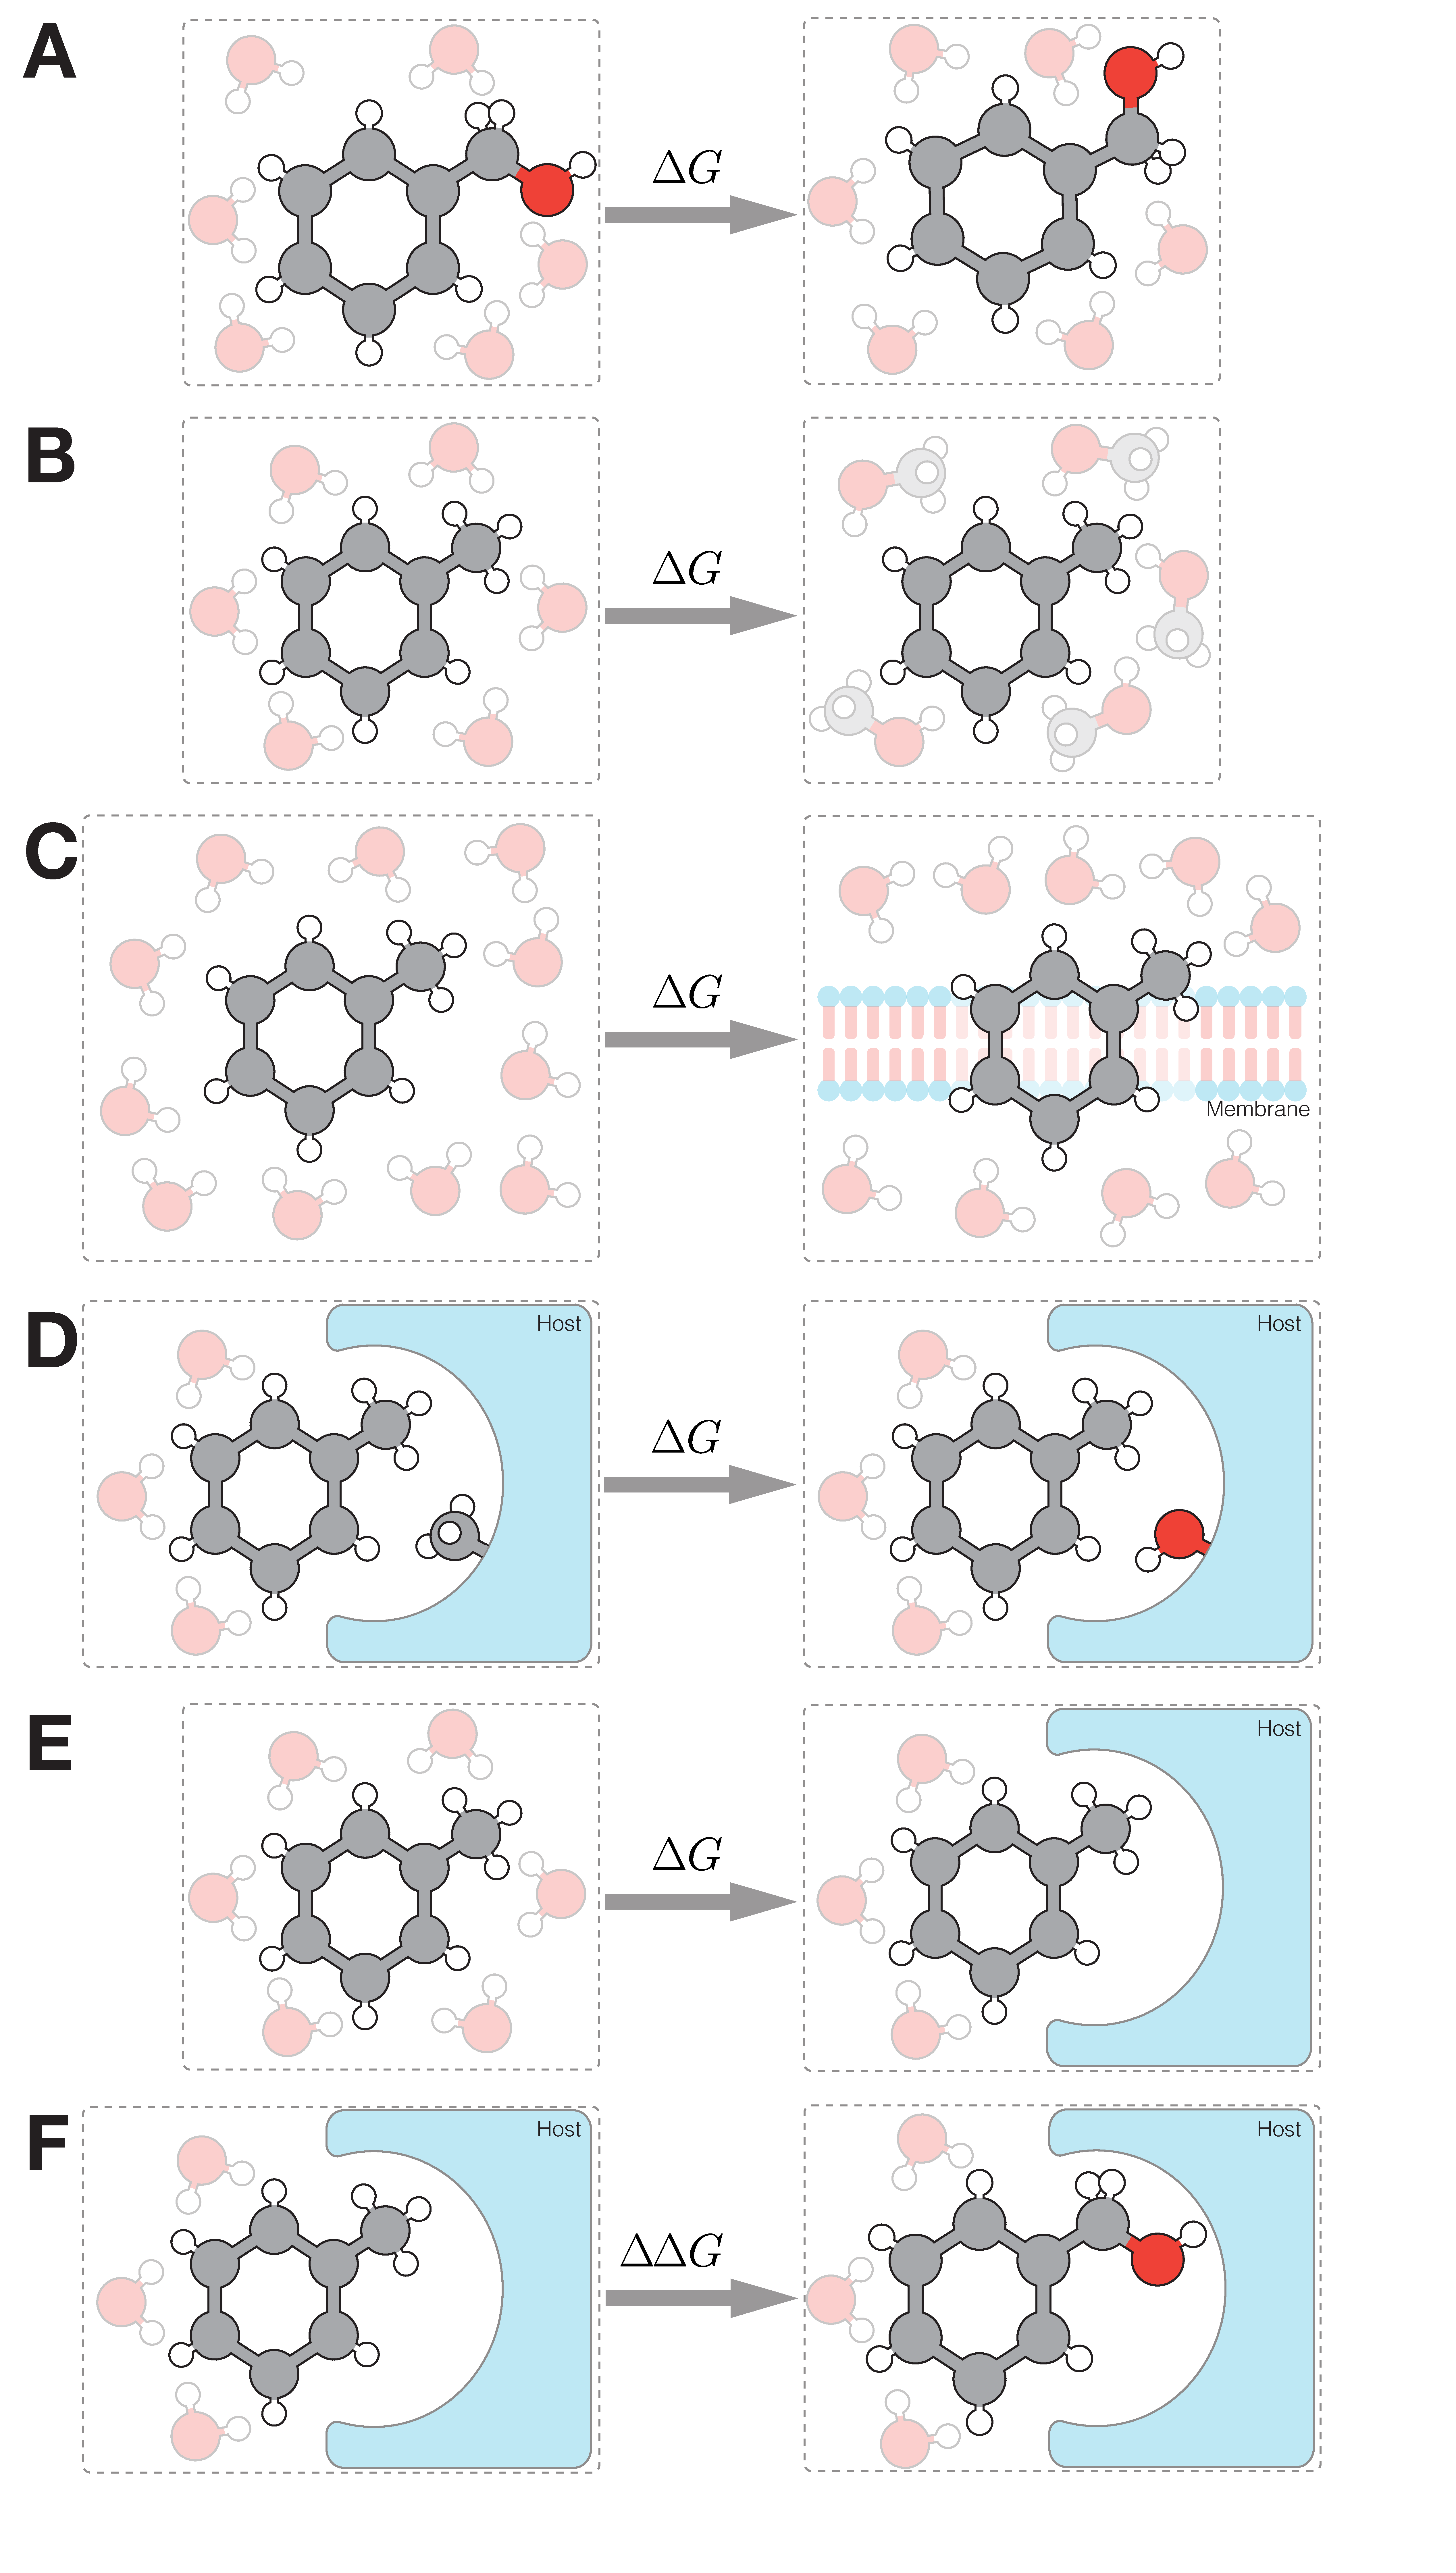
\includegraphics[width=0.95\linewidth]{figures/fig1_what_is_alchemy/Figure.pdf}   
    \caption{\textbf{Illustration of common types of free energies differences that can be calculated using alchemical free energy methods.} \textbf{A}: Change in free energy due to a conformational change of the molecule. \textbf{B}: Partition coefficient such as $\log P$ or $\log D$ depend on a change in free energy between different phases; here, as an example the partition coefficient between methanol and water is shown. \textbf{C}: Free energy difference associated with the insertion of a molecule into a membrane. \textbf{D]: Effect of mutations of protein or host residues on free energies of binding. \textbf{E}: Absolute free energies of binding of a small molecule to a host (e.g. protein), \textbf{F}: Relative free energy of binding of one molecule with respect to another, here toluene and benzyl alcohol.
    \label{fig:fig_what_is_alchemy}
    }
\end{figure}
%
%%%%%%%%%%%%%%%%%%%%
% Prerequesites    %
%%%%%%%%%%%%%%%%%%%%
\section{Prerequisites and Scope}
\label{sec:pre}
\todo[inline, color=green!20]{ASJSM: @everyone This section is up for review to also check flow with intro and rest of document.}
This guide is meant to serve as a comprehensive starting point for new practitioners for free energy calculations.  It assumes moderate experience with molecular simulation packages and concepts, however.  It is also intended to serve as a reference guide with a convenient checklist (Section~\ref{sec:checklist}) for more seasoned practitioners, to help ensure their simulation meet standard alchemical simulation and analysis practices. It can also serve as a set of best practices to ensure simulation robustness and reproducibility which reviewers may wish to consider as they evaluate papers.
%
This guide aims to answer the following questions:
\begin{itemize}
    \item Is my problem suitable for an alchemical free energy calculation? 
    \item How do I choose the right free energy protocol and run it? 
    \item How do I analyze my simulations accurately? 
    \item What software tools are available to perform alchemical free energy calculations? 
\end{itemize}
%
We assume the reader possesses a basic familiarity with the principles of molecular mechanics, molecular dynamics simulations, statistical mechanics, and the biophysics of protein-ligand association. If you feel unfamiliar with some of these concepts please good starting points can be found in these references~\cite{braun2019best, grossfield2018best, klimovich2015guidelines, shirts2012best}. Oftentimes, docking calculations are required to generated initial binding pose for a small molecule for an alchemical calculation, where binding poses are not known, thus some basic familiarty on how to run docking calculations is also expected~\cite{grinter2014challenges}. 
%
As some of the theoretical background can seem daunting, we provide an essentials guide to the theory behind alchemical free energy calculations in Section~\ref{sec:theory}.
In the remainder of this paper, we will cover topics that are key to the preparation~(\ref{sec:prerequisites}), choice and use of correct protocols~(\ref{sec:simulation_protocol_choice}), and finally the best practices that should be used for the analysis of alchemical calculations~(\ref{sec:data_analysis}). 
Particular focus will be given to aspects of the molecular simulations which are unique to alchemical calculations---these include the calculation of transfer free energies (hydration free energies, partition coefficients, etc.), and binding free energies (absolute and relative).
%
While we try to address as many methods and practices as possible, the field of free energy calculations is broad, and there are many advanced topics that are left to future best practices documents focusing on specific issues. 
Below, we provide a non-exhaustive list of topics we have not addressed with some references to provide starting points on these more advanced topics:
\begin{itemize}
\item Covalent inhibition.
\item Free energies of mutation of protein side chains
\item nonspecific binding or multiple binding sites.
\item Complex association stoichiometry (beyond simple 1:1 association)~\cite{awesome reference}.
\item Endpoint free energy methods such as MM-PBSA~\cite{genheden2015mm} and LIE~\cite{gutierrez-de-teran2012linear}
\item Free energy methods that extract the ligand using geometric order parameters and potential of mean force methods~\cite{heinzelmann2017attachpullrelease}
\item Forcefield dependence for protein, ligand, ions, co-solvents, and co-factors. Different studies have looked at the influence of force fields and it is assumed the user has made an adequate choice for the system under study.~\cite{loeffler2018reproducibility, vassetti2019assessment, lopes2015current} 
\end{itemize}
%
For convenience we have also compiled a list of common acronyms, common symbols used, and some essential terminology.
\begin{tcolorbox}[title=Acronyms, colback=blue!10!white]
    \textit{CPU} -- Central Processing Unit\\
    \textit{BAR} -- Bennett Acceptance Ratio\\
    \textit{FEP} -- Free Energy Perturbation\\
    \textit{GPCR} -- G-Protein Coupled Receptor\\
    \textit{GPU} -- Graphics Processing Unit\\
    \textit{MBAR} -- Multistate Bennett Acceptance Ratio\\
    \textit{MCSS} -- Maximum Common Substructure\\
    \textit{MD} -- Molecular Dynamics\\
    \textit{RMSE} -- Root Mean Square Error\\
    \textit{MUE} -- Mean unsigned error\\
    \textit{SAR} -- Structure-Activity Relationships\\
    \textit{TI} -- Thermodynamic Integration
\end{tcolorbox}
%\label{sec:abbreviations}
\begin{tcolorbox}[title=List of Symbols, colback=green!10!white]
$U$ -- potential energy\\
$u$ -- reduced potential energy \\
$\Delta G$ -- free energy \\
$\Delta f$-- reduced free energy \\
$k_B$-- Boltzmann constant \\
$T$ -- temperature
$k_b$ -- rate of binding \\
$K_D$ -- dissociation constant \\
$\lambda$ -- parameter for regulation of the alchemcial free energy path \\
$g$ -- statistical inefficiency
\end{tcolorbox}
\begin{tcolorbox}[title=Common terminology, colback=yellow!10!white]
    ligand - small molecular binding to a larger host molecule such as a protein (recpetor).\\ 
    lead optimization - process of designing a drug candidate from an initial lead compound, considering its affinity and various pharmacokinetic parameters.\\
    thermodynamic cycle - sequence of thermodynamic processes (like changes in temperature, volume or pressure) in which the initial and final state are equal.\\
\end{tcolorbox}
%
%%%%%%%%%%%%%%%%%%%%
% Theory basics    %
%%%%%%%%%%%%%%%%%%%%
\section{Statistical mechanics can tell us why alchemical free energy calculations work}
\label{sec:theory}
\todo[inline, color=green!20]{ASJSM: This section needs to be expanded and give a good introduction to the theoretical background without going into too much detail.}
Why would you want to run an alchemical free energy calculation and why do they work? Suppose you want to compute the binding affinity, or free energy of binding, of a ligand $L$ to a protein $P$, given by:
\begin{equation}
P+L\leftrightharpoons PL
\end{equation}
The equilibrium rate of binding is given by the ratio of concentrations of product $[PL]$ and reactants $[P]$, $[L]$:
\begin{equation}
 K_b^{\circ} = c^{\circ}\frac{[PL]}{[L][P]}.
\end{equation}
In order to define a reference state, the standard state is usually defined as $1 \mathrm{mol}/\mathrm{L}$ and $c^\circ$ is the standard state concentration. Thus, the binding free energy is given by:
\begin{equation}
    \Delta G_{\mathrm{bind}} = -RT\ln K_b^{\circ}.
\end{equation}
One way to estimate the binding rate is by computing the probability of finding the molecular system in the bound state or the unbound state, making use of partition function ratios, i.e. 

\begin{equation}
    \Delta G_{\mathrm{bind}} = -RT\ln\frac{\int_\mathrm{bound} \exp(-\beta U(\mathbf{x}))d\mathbf{x}}{\int_\mathrm{unbound} \exp(-\beta U(\mathbf{x}))d\mathbf{x}}
\end{equation}
Or more generally in a simplified form the free energy difference between the bound and unbound states is:
\begin{equation}
\Delta f \equiv f(\mathrm{bound}) - f(\mathrm{unbound}) = -\ln\frac{Z(\mathrm{unbound})}{Z({\mathrm{bound}})},
\end{equation}
where $Z = \int_\mathrm{bound} \exp(-\beta U(\mathbf{x}))d\mathbf{x}$ represents the configurational integral. 
How can we compute $\Delta G_{\mathrm{bind}}$ from a molecular dynamics simulation? Running a direct simulation of the binding events is too computationally costly, meaning we cannot easily estimate the configurational integrals of the bound and unbound state from the simulation. This is where alchemical free energy simulations come in. We can write down a thermodynamic cycle as seen in ~\ref{fig:fig_binding_thermodynamic_cycle}, for a relative free energy simulation. Based on this cycle we can compute the relative free energy of binding between two compounds $A$ and $B$, by going along the arrow of $\Delta G_{\mathrm{bound}}$, where we introduce a second compound that is similar to the first one. Now $\Delta G_{\mathrm{bound}}$ can be expressed as a ratio of partition functions of toluene (A) and benzyl alcohol (B). 
The defining characteristic of alchemical free energy calculations is the use of a series of alchemically-modified potential functions $U(x; \lambda)$ in which an alchemical parameter $\lambda$ modulates interactions in a manner that cannot occur in real chemical systems.
One or more simulations are used to collect data from a multitude of alchemical states to compute a free energy difference between a chemical state ($\lambda_0$) and another chemical or alchemical reference state ($\lambda_1$),
\begin{eqnarray}
\Delta f &\equiv& f(\lambda_1) - f(\lambda_0) = - \ln \frac{Z(\lambda_1)}{Z(\lambda_0)} , \label{equation:dimensionless-free-energy-difference}
\end{eqnarray}
where the dimensionless free energy $f(\lambda) \equiv \beta F(\lambda)$ is given in terms of partition functions $Z(\lambda)$,
\begin{eqnarray}
Z(\lambda) &=& \int dx \, e^{-u(x; \lambda)} .
\label{equation:partition-function-definition}
\end{eqnarray}
Here, the inverse thermal energy $\beta \equiv (k_B T)^{-1}$ where $k_B$ is the Boltzmann constant and $T$ is the absolute temperature, and the \emph{reduced potential} $u(x; \lambda)$~\cite{shirts2008statistically} is generally given by a trace over thermodynamic parameters with their conjugate dynamical variables,
\begin{eqnarray}
u(x;\lambda) &\equiv& \beta \left[ U(x;\lambda) + p \, V(x) + \sum_{i=1}^N \mu_i \, N_i(x) + \cdots \right] . \label{equation:reduced-potential}
\end{eqnarray}
Here, the collection of thermodynamic and alchemical parameters $\theta \equiv \{\beta, \lambda, p, \mu, \ldots\}$ defines a \emph{thermodynamic state}.
The physical transformation of interest---such as a protein-ligand association process, or transfer free energy among phases---may involve a thermodynamic cycle that requires several free energy differences $\Delta f$ to be computed in order to produce an estimate of the overall desired quantity.

\begin{figure}
    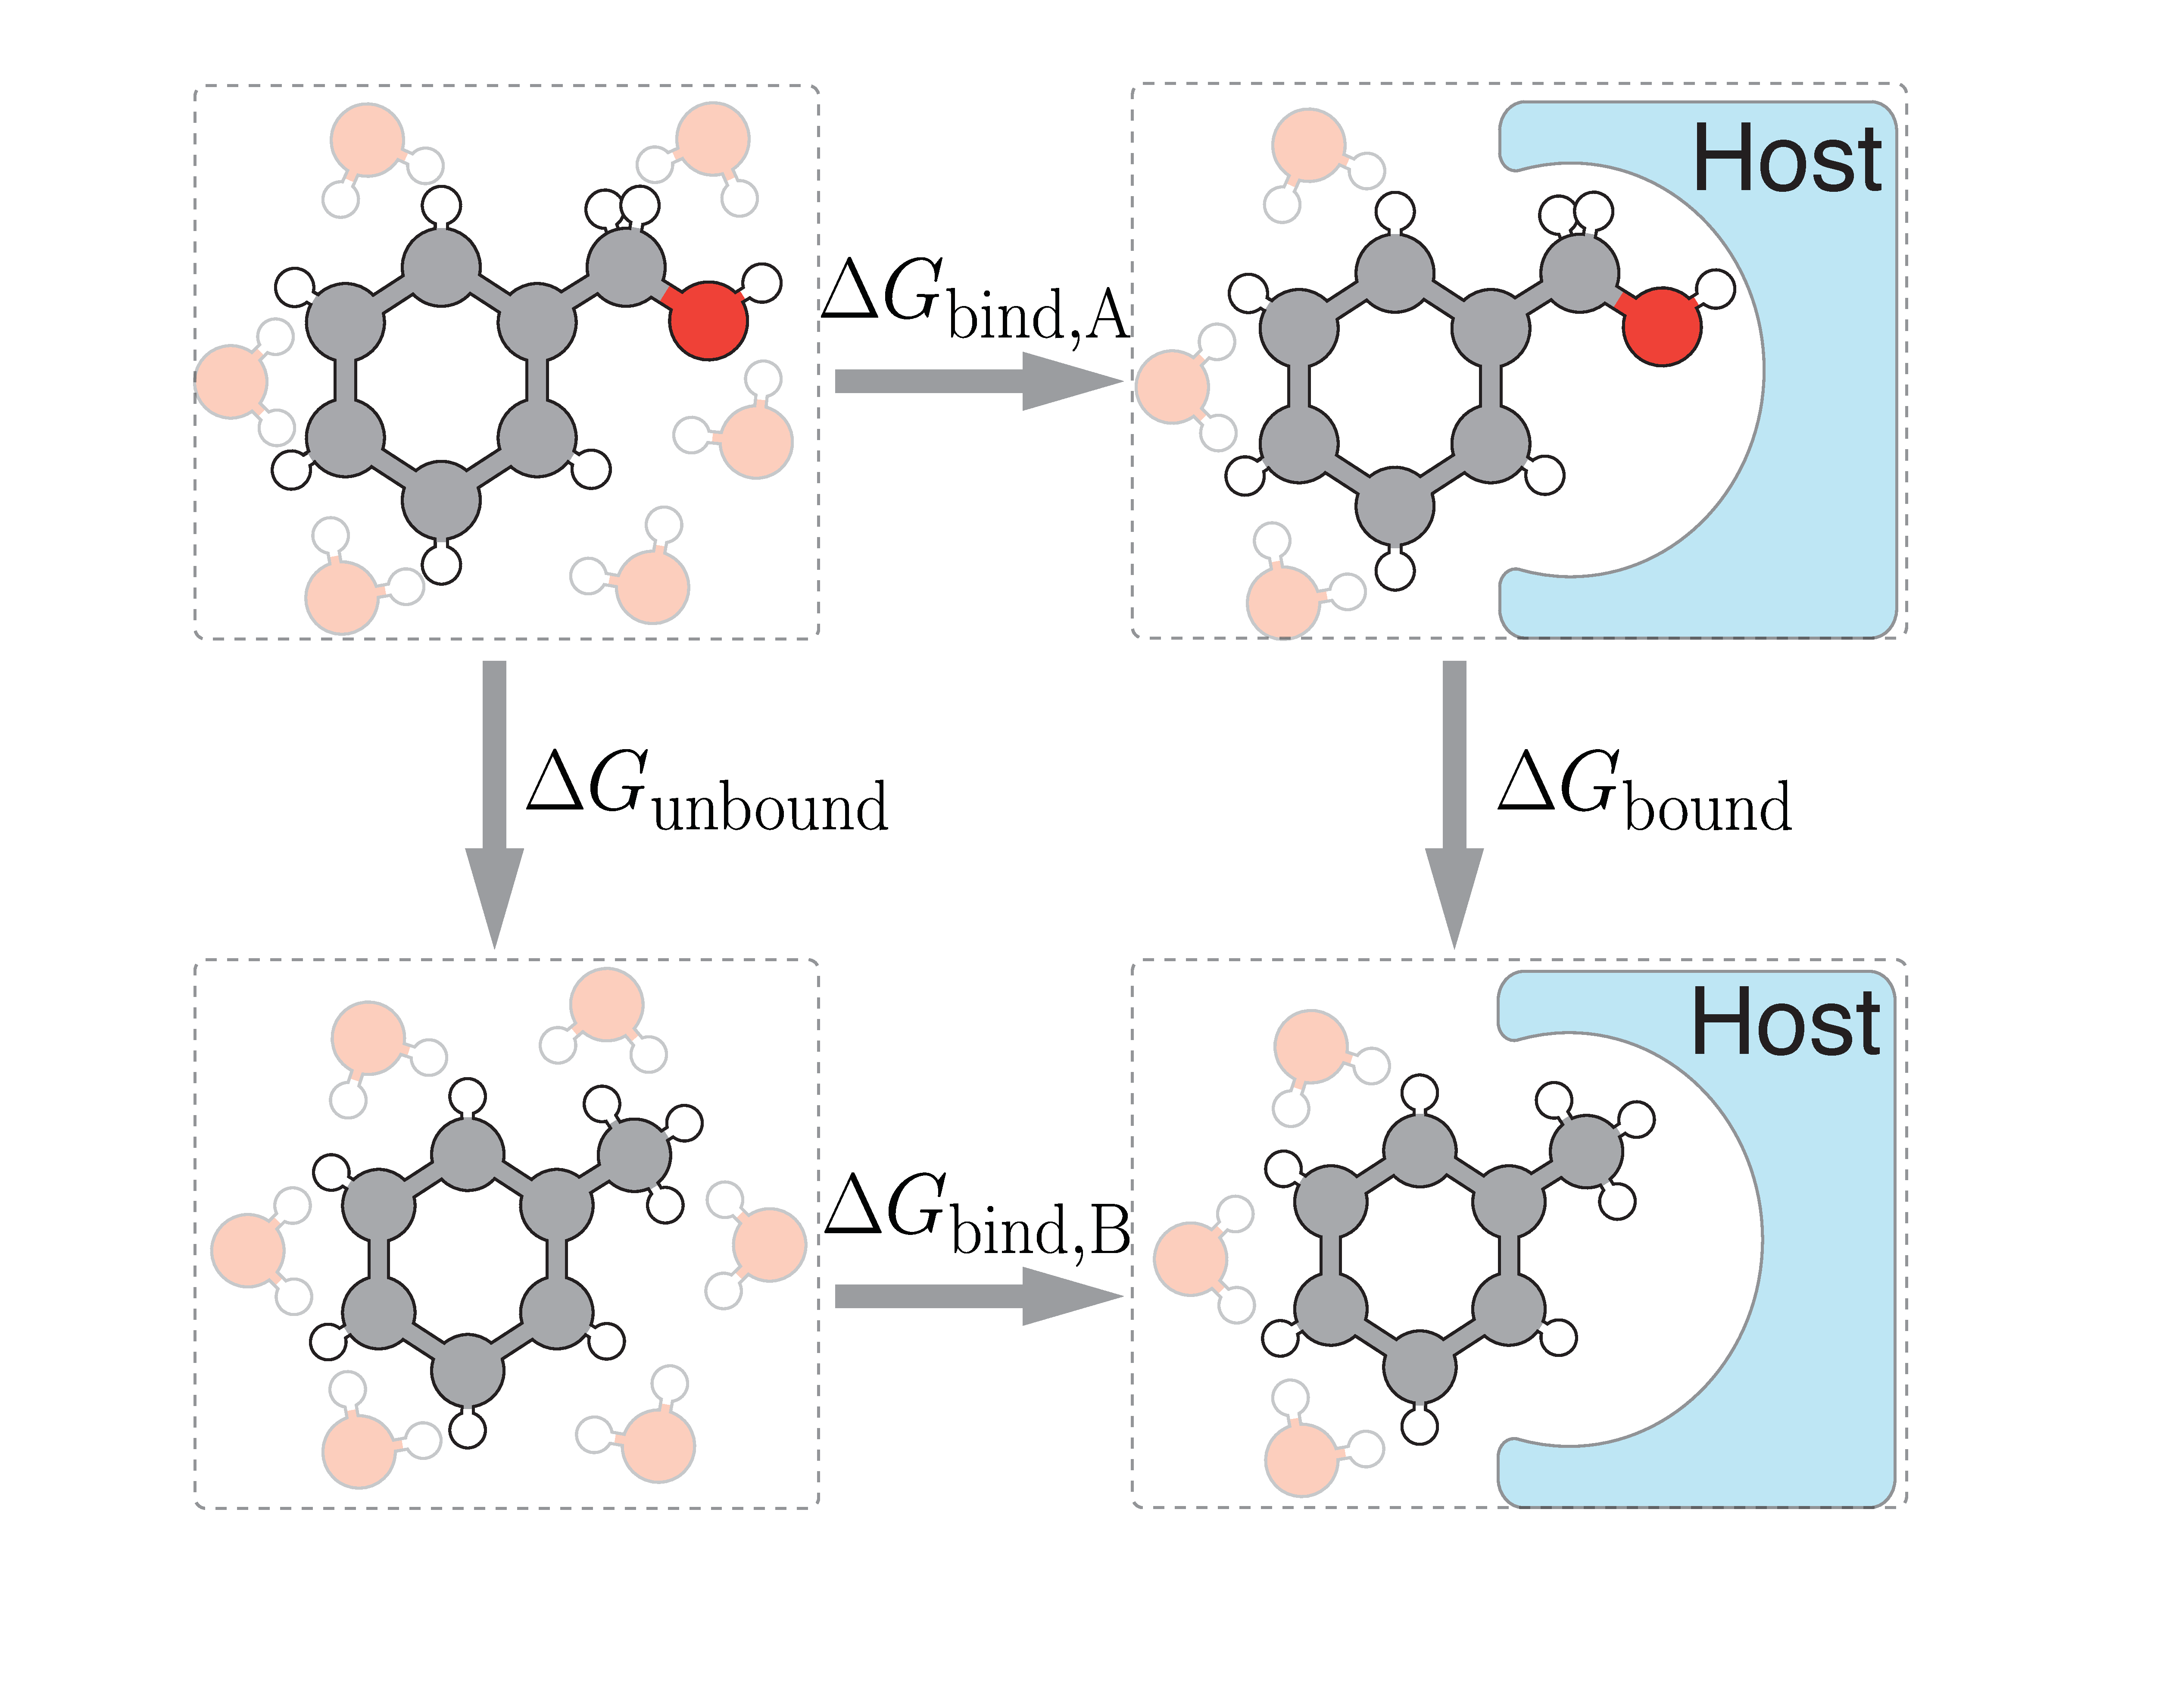
\includegraphics[width=0.95\linewidth]{figures/fig2_therm_cyc/Figure.pdf}
    \caption{{\bf Thermodynamic cycle for computing the relative free energy of binding ($\Delta \Delta G$) between two related small molecules to a supramolecular host.}
    The relative binding free energy difference between two small molecules, $\Delta \Delta G_{\mathrm{bind}, A \rightarrow B} \equiv \Delta G_{\mathrm{bind}, B} - \Delta G_{\mathrm{bind}, A}$---here benzyl alcohol (top) to toluene (bottom)---can be computed as a difference between two alchemical transformations, $\Delta G_\mathrm{bound} - \Delta G_\mathrm{solvated}$, where $\Delta G_\mathrm{bound}$ represents the free energy change of transforming $A \rightarrow B$ in complex and $\Delta G_\mathrm{solvated}$ the free energy change of transforming $A \rightarrow B$ in solvent.}
    \label{fig:fig_binding_thermodynamic_cycle}
\end{figure}



%%%%%%%%%%%%
% Step 0   %
%%%%%%%%%%%%
\section{What can be expected from alchemical simulations?}
\label{sec:step0}
\todo[inline, color={green!20}]{ASJSM: @everyone please review this section}
When starting an alchemical free energy project you need to determine if an alchemical free energy calculation is the appropriate strategy by initially counting the cost of your
project: Can you even hope to tackle the problem with available resources and, if successful, will it
be worth it?
\subsection{How accurate are alchemical free energy calculations?}
\label{subsec:expectation}
%
Current alchemical free energy calculations seem to achieve, in favorable cases, RMS errors around 1-2 kcal/mol depending on force field, system, and a variety of other factors such as simulation time, sampling method, and whether the calculations employed are absolute or relative. A small selection of benchmark datasets and case studies can be found in section~\ref{sec:benchmark} at the end of this document.
However, the domain of applicability is a significant concern~\cite{sherborne2016collaborating, cournia2017relative}, especially for relative calculations, which typically require a bound structure of a closely
related ligand as a starting point. Additional factors such as slow protein or ligand rearrangements, uncertainties in ligand binding mode, or charged ligands can make these calculations far less reliable and more of a research effort.
%
It is worth noting that the accuracy of free energy calculations is highly variable across different protein targets, and likely across different ligand chemotypes as well. For instance, FEP+ with OPLS3 achieves an RMSE of 0.62 kcal/mol for a set of 21 compounds binding to JNK1 kinase, yet only an RMSE of 1.05 kcal/mol for a set of 34 compounds binding to P38$\alpha$ kinase~\cite{harder2016opls3}. Furthermore, perturbations for the same chemotype in different pockets of the BACE enzyme gave varied errors~\cite{keranen2017acylguanidine}
\todo[inline,color={green!20}]{JDC: It's important to be clear on what error is being reported: $\Delta G$ after shifting by a constant to minimize the RMSE, unshifted $\Delta G$, $\Delta \Delta G$ of computed edges, or $\Delta \Delta G$ of all edges. Note that computed edge $\Delta \Delta G$ RMSE significantly underestimates the error of all edge RMSE: \url{https://github.com/jchodera/jacs-dataset-analysis} ASJSM: Can we incorporate your analysis in this section as an example? Maybe this is something that needs to be addressed properly in the analysis section and only referenced here?}
We thus recommend that retrospective study for a particular target and a particular chemical series be performed to establish the relevant accuracy of free energy calculations for each particular application case.
%
\subsection{How reproducible are alchemical free energy calculations?}
\label{subsec:reproducible}
Finite computing resources necessarily limit the generated number of uncorrelated samples of potential energy surfaces, and therefore alchemical free energy calculations only give free energy estimates to within finite precision. An important consideration is how reproducible alchemical free energy calculations are in practice. In simple cases such as absolute hydration free energies of small organic molecules, or relative hydration free energy calculations between structurally similar small organic molecules, it should be possible to obtain highly precise estimates with a given software package (with a sample standard deviation under 0.01 kcal/mol). For more complex use cases such as protein-ligand binding free energies the repeatability is often substantially worse. A good practice is to perform two or three runs of the same perturbation to assess repeatability with a given protocol. The sample standard deviation will give a crude estimate of the reliability of the estimates, and whether the precision is sufficient for the problem at hand. Where this is practical, a more stringent test is to use different input coordinates for each repeat run. 
%
Note that these issues concern calculations carried out with a single software package, but simulation package variations can introduce additional issues. Such issues of reproducibility of free energy calculations across different simulation packages have attracted attention recently. Greater variability is expected due to methodological differences such as integrators, thermostats, barostats, treatment of long-range electrostatics, and potentially other factors. For absolute and relative hydration free energies of small organic molecules a variability of ca. 0.2 kcal/mol between popular simulation packages has been reported. \cite{REF Reproducibility of hydration free energies Loefler et al.  JCTC 2018} In the recent SAMPL6 SAMPLing challenge a larger variability of 0.3 to 1.0 kcal/mol was noted in the computed absolute binding free energies of host/guest systems even though similar input and simulation parameters were used \cite{Ref Rizzi et al SAMPLing biorxiv} and, in many cases, single-point energies were identical or nearly so. Further work is needed to ensure reproducibility of alchemical free energy calculations across implementations to guarantee that force-field development efforts lead to transferable potential energy functions. 
%
\subsection{Is my problem suitable for alchemical free energy calculations?}
\label{subsec:suitability}
Before even planning free energy calculations to study binding to a
particular target, it is important to assess what is known about the
system and its timescales and its suitability for free energy
calculations, as well as the \emph{purpose} of the calculations and
the amount of available computer resources. In some cases, predicting
accurate binding free energies for a particular target might be a
\emph{more} challenging effort than simply measuring them! This is
often the case when dealing with database screening problems, where
compounds might be easily and quickly available commercially for
testing and free energy calculations could consume a much larger
amount of resources. Free energy calculations thus typically only
appeal when (slow or costly) synthesis would be required to do
experiments or experiments are otherwise cost-prohibitive.
%
Sometimes free energy calculations can provide answers that are not
readily available from experiments.  For example, type II kinase
inhibitors selectively bind to different kinases in the so-called
DFG-out conformations (cite Kuriyan).  The selectivity of such
inhibitors may be attributed either to their differential binding to
different kinases in the DFG-out conformations, or to different
stability of the DFG-out conformations of different kinases.  Let
$K_C$ be the equilibrium constant between DFG-in and DFG-out
conformations of one kinase, and $K_D^\ast$ be the dissociation
constant of a type II inhibitor against this kinase, the apparent
binding constant of this inhibitor against this kinase is then
\begin{equation}
  K_D = K_D^\ast \frac{1 + K_C}{K_C}
  \label{eqn:conformational-binding}
\end{equation}
%
Since binding experiments cannot resolve $K_D^\ast$ and $K_C$ individually, such experiments cannot address the basis of selectivity of the type II inhibitors.  Absolute binding free energy calculations, in contrast, can take advantage of the slow kinetics of DFG-in/out conversion, and estimate the conformation-specific binding constant $K_D^\ast$, thus yielding clues as to the source of selectivity.
%
\subsection{Is the expected accuracy of the computation sufficient?}
\label{subsec:accuracy}
The requisite level of accuracy is another important consideration ---if the
goal is to guide lead optimization when many compounds will be
synthesized, free energy calculations can be appealing even with
accuracy in the 1--2 kcal/mol range~\cite{mobley2012perspective}, but if the number of compounds to be synthesized is very small, this accuracy may not be enough to provide
much value.
%
Here we include a simple estimate of the value provided by alchemical
free energy calculations in lead optimization.  Let $P(\Delta\Delta
G)$ be the probability distribution of the changes in the binding free
energies of a new set of molecules during one round of lead
optimization, and let $P(\Delta\Delta G^\dagger|\Delta\Delta G)$ be the
conditional probability of the binding free energy change computed by
the free energy calculations, $\Delta\Delta G^\dagger$, given the actual
change $\Delta\Delta G$.  The latter conditional probability can be modeled
by a normal distribution
\begin{equation}
  P(\Delta\Delta G^\dagger|\Delta\Delta G) = \frac{1}{\sqrt{2\pi\sigma^2}}
  \exp\left(-\frac{(\Delta\Delta G^\dagger - \Delta\Delta G)^2}{2\sigma^2}\right),
  \label{eqn:free-energy-distribution}
\end{equation}
where $\sigma$ signifies the accuracy of free energy calculations.
Here we assume that there is no systematic bias in the free energy
calculations, i.e., on average, the free energy change computed by
free energy calculations agrees with the actual free energy change.
%
In lead optimization guided by free energy calculations, we only
synthesize and experimentally test molecules that are predicted to
have favorable free energy changes.  We are thus interested in how
often that a molecule predicted to bind stronger actually turns out to
bind stronger.  In other words, we are interested in the conditional
probability:
\begin{equation}
  P(\Delta\Delta G<0|\Delta\Delta G^\dagger<0).
  \label{eqn:true-positive}
\end{equation}
%
For illustrative purposes, we assume that the actual changes in the
binding free energies for a set of new molecules also follow normal
distribution, that the standard deviation in the changes is $RT\ln 5$
(corresponding to a 5-fold change in the binding affinities), and that
1 in 10 new molecules have increased binding affinity ($\Delta\Delta G
\leq 0$).  Under such assumptions, the conditional probability in
Eq.~\ref{eqn:true-positive} can be easily computed.  If the accuracy
of free energy calculations is $\sigma = 1$ kcal/mol, $P(\Delta\Delta
G<0|\Delta\Delta G^\dagger<0) = 0.35$, which means that out of every
10 molecules selected for predicted favorable free energy change, on
average 3.5 molecules will have actual favorable free energy change.
In other words, selection by free energy calculations yields 3.5 times
more molecules of improved affinities than selection without free
energy calculations.
%  
Available computational resources and timescales of motion also factor
into this initial analysis. An individual free energy calculation
involves simulations at many different intermediate states (perhaps
20-40 or more) and each of these must typically be long enough to
capture the relevant motions in the system. If such motions are
microsecond events or longer, the computational cost of running 20-40
microsecond or longer simulations for each of $N$ ligands may become
prohibitive, or at least should be carefully considered. 
%
\subsection{Can I afford the calculation?}
\label{subsec:affordability}
Furthermore, are available computational resources sufficient that throughput will be
reasonable compared to needs of experimental collaborators working on
this system? How many ligands ($N$) can you afford to handle given
your computational resources? As cloud computing becomes more available, in-house GPU clusters may not be necessary if calculations are not run on a regular basis.
This analysis should be done up front, part of ``counting the cost''
of involvement in a particular project. In some cases, the analysis may conclude that free energy calculations will not be feasible for the proposed problem.
Here, by ``cost'', we refer not just to financial cost of the calculations relative to experiments, but also time -- can the calculations can be run faster than experiments are done? How will the relevant resource and opportunity costs factor in? Both computation and experiment require human time, supplies (of different sorts), and equipment. In the extreme limit, for example, it would not make sense to spend a month running a binding free energy calculation if the equivalent experiment could be done in a day with resources already on hand. Such issues should be considered before deciding to conduct binding free energy calculations.
%
\subsection{Is an exploratory study what I want?}
\label{subsec:exploration}
An additional consideration is how much is known about your particular
target, ligand binding modes in the target, and any relevant motions
-- essentially, has it been studied enough to know whether it might be
suitable for free energy calculations? It is important to know if the system has hardly been studied, because should the initial calculations perform poorly, the effort may turn into an attempt to understand the relevant sampling, force field, or system preparation problems.
%
If you are unsure whether your project is feasible, one option may be
to conduct a short exploratory study to assess tractability for just a very small
number of ligands. This can be sufficient to get an initial
idea of feasibility and accuracy of the calculations for the
proposed target.
%
\section{How should alchemical simulations be applied to drug discovery?}
\label{sec:drugdiscovery}
\todo[inline, color={green!20}]{ASJSM: Merge/tidy of what can I expect from my simulation, drug discovery aspects and simulation prerequisites, there are some duplications there at the moment, happy for restructuring ideas.  }
%
Many practitioners expect alchemical methods to provide valuable guidance for drug discovery, and to exhibit accuracy superior to most  alternative approaches for suitable targets~\cite{kuhn2017prospective}. It has been stressed that successful application in industry may require considerable knowledge of the "domain of applicability" of free energy calculations -- where they work well and where they will not ~\cite{sherborne2016collaborating}. Successful application also requires robust protocols for preparing, submitting and analysing alchemical calculations. In this regard, the issues mentioned in the previous section such as understanding the suitability and timescales to capture the structure activity relationships (SAR), and performing up-front tests of performance are all relevant to drug discovery applications. Without venturing too far into details of system setup, which is beyond the scope of this article, we highlight some critical factors affecting accuracy and successful application. 
%
\subsection{Capturing the experimental conditions}
The calculations aim to capture the alchemical change from one ligand to another as accurately as possible. Therefore, it is necessary to consider details of the experimental setup, such as pH. Biological assays are usually run at neutral pH but this is not always the case, and protein and ligand preparation protocols should reflect this. In more detail, the formal charge, or tautomeric state of the small molecules can change within a series of analogs. The change of pKa is a common medicinal chemistry strategy to modify drug properties and would normally require explicit effort to incorporate into alchemical calculations. Also, to ensure modeling matches experiment, we need to ensure that we simulate the same system -- which requires understanding what protein construct is used in the bioassay. For instance, does the X-ray that is to be used for the calculations match the construct used for screening (i.e. catalytic vs full length, monomer vs dimer etc) (CITE https://www.nature.com/articles/s41598-018-23039-5)? Also, were certain co-factors or partner proteins required in the bioassay? 
%
\subsection{Is my binding mode accurate?}
As also mentioned, good performance of alchemical FE calculations requires an accurate representation of the ligand binding mode, which often is estimated based on X-ray crystallography for a related ligand. If more than one structure is available, the modeler should pay attention to choose the most suitable. The quality of the structure can be a concern, and the reader is referred to work of Warren et al. for a detailed discussion of choosing optimal structures for structure-based modeling~\cite{warren2012essential}. It is also useful to study the structure activity relationship and understand the expected impact in the binding site, whether side chain movement in the protein will be required, and whether there evidence of this in any alternative X-ray structures of the same protein. Often, only one protein and water configuration is used for a series of alchemical FE calculations, so this needs to be capable of accommodating the smallest through to largest ligands in a way that allows stable and well behaved simulations. This can be a practical limitation for the alchemical changes that are feasible, though a simple work-around can be to separate compounds into sub-series for different calculations. If multiple structures are available there is some evidence the higher affinity complex can give better performance~\cite{perez-benito2019predicting}, at least in some cases. However, ligands and proteins can also undergo unexpected changes in binding mode for related ligands, which can make these issues more complex to deal with.

\subsection{Input setup and scale of calculations}
In a drug discovery setting it is normal to consider dozens (or more) of ligands and it is necessary to align them in the binding site. There is no detailed study of how different alignment approaches may affect results, but the user should be aware of some practical considerations. Tools are available to compare the ligands and build the hybrid topologies that define the changes between one ligand and another~\cite{loeffler2015fesetup,hedges2019biosimspace,gapsys2015pmx}. In simple terms, providing poor alignment to these tools will make this job harder. Therefore, docking ligands with no restraints is not usually the best method for defining the ligand inputs, instead a core restrained docking can provide satisfactory outcomes, but in this case one still should pay careful attention to consistency of alignment for identical substituents. Another alternative is to manually edit the same core with the changing substituents. This provides assurances that coordinates for the non-perturbed structures remain identical and aromatic substituents for instance obey consistent dihedral angles but is not feasible for many compounds and therefore automation can be desirable. 

Finally, the role of water in ligand binding is now well understood and it can be crucial to capture the changes in binding site solvation during ligand binding. Can crystallographic waters be retained? Do they clash with some of the larger ligands used in the FEP? If so, how will the water be incorporated for smaller ligands that require the water – consider pre-solvation methods such as GCMC steps~\cite{michel2010prediction}. Other tools such as WaterMap or open source equivalents (SSTmap, others) can be used to define water structure for systems with no experimental evidence of water sites. Before launching large numbers of alchemical free energy calculations it is recommended to test the system using classical MD simulations and limited numbers of alchemical perturbations. Metrics such as ligand and protein RMSD and RMSF can be inspected, along with visual inspection of simulations, to ensure the system is stable and likely to be suitable for FE calculations. 

Running binding FE calculations in a drug discovery application will typically require the use of software or tools to facilitate the calculations of many compounds. The commercial implementation from Schr\"{o}dinger, FEP+, uses a graphical user interface and once the user has calculated any missing force field parameters, calculations can be prepared and submitted within minutes. The software builds the network of perturbations, connecting similar compounds based on LOMAP methodology~\cite{liu2013lead}, all inputs for the Desmond simulations are built automatically and the job can be saved or run immediately on available GPUs. The cost of this software is often prohibitive but alternative tools are becoming available to allow relatively straight forward running of alchemical FE calculations with other software~\cite{gapsys2015pmx, loeffler2015fesetup, song2019using, gapsys2020large,  jespers2019qligfep}. One consideration at this point is to define the perturbations suitable for the application. For instance, if the goal is to accurately assess the relative binding energy of a small number of compounds, possibly with challenging synthesis, the map of perturbations may contain as many connections between compounds as affordable. However, when running calculations on hundreds of compounds a so called ‘star-map’ can be used that just contains one connection per compound: perturbing every compound to a central ligand, typically the crystal structure ligand~\cite{konze2019reactionbased}. In this way the top-ranking examples can be readily identified and submitted to additional calculations in a second round. 
%
\subsection{Making predictions, understanding errors}
\label{subsec:predictions}
For prospective drug discovery applications there are several other considerations including understanding likely errors and taking selection bias into account. It is crucial when proposing compounds for synthesis to have some idea of the underlying error or uncertainty in the predictions. A retrospective assessment can give an indication of prospective performance for similar molecules~\cite{ciordia2016application}. Beyond this, several parameters provide useful indicators of performance. Results suggest MBAR errors greater than 0.3 kcal/mol for perturbations can be indicative of inaccuracy~\cite{perez-benito2019predicting}. In addition, the hysteresis can be checked by comparing the difference for forward and reverse perturbations of the same structural change, or in the case of large maps of perturbations cycle closure errors~\cite{wang2013modeling} indicate problematic perturbations involved in cycles connecting many compounds. Selection bias, as described above, can be problematic in prospective applications as there is normally an aim to focus on only a narrow range of predicted activity (i.e. the most active). Thus, correlation between prediction and subsequent experiment may lead to disappointment but corrections can be applied based on previous recommendations~\cite{abel2017critical}. 

In summary, the successful use of alchemical calculations in drug discovery requires working in the domain of applicability, using a high quality X-ray structure of the target compounds, and testing the approach retrospectively to ensure the system setup is well-behaved. Always assess your confidence in the resulting predictions and communicate this when discussing with experimentalists. Consider performing repeat calculations for at least some of the perturbations in the study. In a drug discovery setting it is inevitable to consider larger virtual libraries. In these cases again evaluate if shorter simulation time per $\lambda$ window can be sufficient for a ‘virtual screening’ mode of application. It is expected that future tools may allow efficient exploration of large virtual libraries. There are many accounts of success of alchemical FE calculations, the methods show good performance towards the goal of binding energy prediction. However, it is important to have realistic expectations. 

Structure based drug design projects are often capable of improving potency relatively quickly, even with only limited application of computational approaches and the range of activity narrows to just two-to-three log units. It may seem hard to have impact with substantially different, more potent, stand-out compounds in this scenario, but binding energy prediction can still be extremely useful for ensuring activity is maintained as other properties are optimized. An interesting cost benefit analysis has shown the value of activity prediction, see discussion above and articles such as~\cite{mobley2012perspectiv}. From a drug discovery point of view, FEP is expanding its domain of applicability, and there are reports of success using homology models and GPCRs for instance, as well as enabling charge change and scaffold hopping, but these systems are undoubtedly more difficult.  In the meantime, the use cases are expanding to resistance prediction, disease mutation prediction, solubility prediction – an exciting future for alchemical FE calculations. 
%
%
%
%%%%%%%%%%%%%%%%%%%%%%%%%%%%%
% Simulation prerequisites  %
%%%%%%%%%%%%%%%%%%%%%%%%%%%%%
%
\section{Simulation prerequisites}
\label{sec:prerequisites}
The alchemical free energy protocols, that are discussed in Section~\ref{sec:simulation_protocol_choice}, are defined for a specific type of free energy calculation, i.e. a free energy of binding or a free energy of hydration. Depending on the type of simulations different considerations have to be made for ligands, solvent, and host molecules (in the case of the estimation of free energies of binding).
\subsection{Free energies of binding}
\label{subsec:binding}
In principle in the limit of sufficient conformational sampling, the free energy changes estimated from an alchemical free energy calculation should be independent of the system's initial coordinates. However, in practice because simulations of thermodynamic states are of finite duration (typically currently 1-100 ns per state) this is only true for certain classes of alchemical free energy calculations such as relative or absolute free energies of hydration of small and relatively rigid organic molecules. Host-guest or protein-ligand complexes typically exhibit slowly relaxing degrees of freedom that exceed significantly the duration of an alchemical free energy calculation. It is therefore generally important to carefully select input coordinates to obtain satisfactory results. 
The following questions may be relevant before diving into the simulation setup.
% 
\begin{itemize}
    \item Do I have one or multiple good host structures? (e.g. a good resolution X-ray crystal of the protein target)
    \item Do I have information on one or all of the ligands binding sites (e.g. a X-ray structure)
    \item Should I include buried waters, or other small molecules that can be found in an X-ray structure.
    \item Are my ligands part of a congeneric series? (simple R group substitutions around the same scaffold)
    \end{itemize}
%
\paragraph{Are there good X-ray structures available?}
As for any simulation, care should be taken in selecting available X-ray structures in the protein databank and potentially choosing multiple structures initially, to account for variability in receptor conformations as well as accuracy of available X-ray structures. Typically, clustering of receptor structures can be used to identify different receptor conformations near the binding site, as well as assessing relevant side chain placements from the X-ray structure, see for example~\cite{mey2016blinded}. In terms of set up and other choices following general best practice guidelines is advisable~\cite{braun2018best}.
%
For binding free energy calculations using a congeneric set of ligands and therefore likely to be most suited to a relative free energy protocol (see~\ref{sec:simulation_protocol_choice}). Other than the choice of forcefield for the parameterization of the ligands, some care has to be taken selecting binding poses for these ligands. Generally a common assumption for a congeneric series is that the binding mode is conserved. Therefore, if an X-ray structure of one of the ligands is available, this should be used to position the ligands in the putative binding site in an energetically reasonable conformation that entails no steric or electrostatic mismatch with the receptor. Checking the X-ray structure versus the experimental electron densities is important, as the resolution of part of the ligand or important sidechains may be based on the interpretation of the crystallographer rather than the available electron density. For example, looking at a cyclohexane ring density, a chair conformation is vastly more likely than that of a boat and may just be poorly assigned. 
%
\paragraph{How to deal with different binding modes?}
Generally, binding modes within congeneric series are conserved~\cite{wacker2010conserved}, however, exceptions exist~\cite{brandt2011congeneric,nazare2005probing}, and weaker binding compounds are more likely to adopt different binding modes (REFS). There may also be ambiguity about the relative orientation of substituents. A known issue involves a 180 degree flip in the dihedral angle of a 6-membered aromatic ring leading to a different spatial position of ortho- or meta- substituents that otherwise should overlap within a series. The 180 degree flip of the ring may not occur enough during simulations to overcome the starting configuration bias. Another scenario may be equatorial and axial substituted saturated rings (e.g. cyclohexane derivatives). This situation may be addressed by explicitly modelling different binding modes of the same ligand and combining later computed free energy differences for different binding modes into a relative free energies of binding~\cite{kaus2015how}.
%
\paragraph{Have you considered sterioisomers and enationmers?}
Congeneric series can contain stereoisomers or enantiomers, making sure that you model the correct one is important. For racemates, the relative abundance of each stereoisomer is normally not known. Therefore, the experimental activity associated with just one conformation is more uncertain. However, the modeling typically uses just the bioactive conformation that best fits the active site. Clearly this introduces the chance for higher error versus experiment. Nevertheless, if all compounds in the congeneric series are racemic, originating from similar synthetic procedures with an expected similar abundance of stereoisomers, then the differences may cancel and the trend in calculated and observed binding energies may be robust. Nevertheless, we can see that care and further testing is needed in this scenario, and the quality of the predictions may suffer.   
%
\paragraph{Conserved binding site waters can play an important role in binding free energies}
Another aspect to look out for are binding site water molecules that may form water mediated protein-ligand interactions, particularly in situations where exchange with bulk water may be slow on the simulation timescales. This happens typically in buried binding site. Overlaying multiple protein X-ray structures can identify conserved or just additional water molecules that can be useful to include. In cases where water molecules are known to play an important role in the binding, software implementations that use water sampling facilitated by Grand Canonical Monte Carlo methods may be useful. For examples see HSP90 as formed part of the D3R grand challenge 2015~\cite{mey2016blinded},A2A~\cite{brucemacdonald2018ligand}, MUP~\cite{ross2015water}, and others~\cite{michel2009energetics}.
%
\paragraph{How to align congeneric series}
Input coordinates for a congeneric series may be generated by docking calculations, or by ligand alignment using maximum common substructure algorithms. The latter tends to produce alignments that are more conserved and more consistent free energy changes across a dataset, but will struggle to yield reasonable results for relative binding free energy calculations that involve a significant binding mode rearrangement. This may also lead to steric clashes with the receptor coordinates of the reference ligand if structural rearrangements are needed to accommodate different members of the congeneric series. Small steric clashes may be resolved during subsequent simulation equilibration prior to data collection, but there is a risk that the complex relaxes to an alternative metastable state. 
%
An additional consideration arises for single topology relative free energy calculations. In this class of alchemical free energy calculations it is necessary to generate a molecular topology that may describe the initial and final states of the perturbation (see different topologies as seen in Fig.~\ref{fig:fig_topology}). In cases where the end-states have high topological similarity and high structural overlap this is relatively straightforward and typically handled by use of maximum common substructure calculations. In situations where the end-state topologies differ significantly, or there is relatively little spatial overlap between the two end-states some user intervention may be necessary to produce a satisfactory input topology.
%
If the binding site location is uncertain but the structure of the receptor is well defined and plausible binding sites are identified, it may be more useful to chose an absolute free energy protocol to compute the standard free energy of binding of the ligand to a set of binding sites. This requires the user to prepare input files describing the bound conformation in different putative binding sites (REF). The apparent binding free energy of the ligand may be obtained by combining the individual binding site free energies, which also indicate where the ligand is more likely to bind. In this case a docking program can generate initial structures. Different commercial and none commercial tools are available, such as: rDock, Autodock Vina, Glide, or Flare to name a few~\cite{ruiz-carmona2014rdock, trott2010autodock, friesner2004glide, cheeseright2006molecular}. 
If the putative binding sites are not apparent, for instance due to significant induced-fit effects, it may be challenging to obtain meaningful free energies of binding. One may have to account for the free energy change for forming a binding site in the target receptor which may not be feasible in FE simulation timescales. Another key application for absolute binding free energies is to study chemically different ligands, that do not share a common scaffold, but bind at the same site or the same site of similar proteins~\cite{aldeghi2015accurate}.  
%
\subsection{Free energies of hydration or partition coefficients}
\label{subsec:hydration}
Preliminary considerations necessary for using free energy methods to compute partition coefficients are generally more straight forward. For example, a 3D minimised structure of the solute can be generated with a simple tool such as openBabel and solvated to prepare the input  to compute a free energy of hydration~\cite{oboyle2011open}. However, in these cases a careful choice of forcefield, as well as water models or organic solvents is essential. See for example~\cite{bosisio2016blinded,rustenburg2016measuring} for a good discussion on these choices. 
%
%%%%%%%%%%%%%%%%%%%%%%%%%%%%%%%%%%%%%%%%%%%%%%
% What simulation protocol should I choose   %
%%%%%%%%%%%%%%%%%%%%%%%%%%%%%%%%%%%%%%%%%%%%%%
\section{What simulation protocol should I choose?}
\label{sec:simulation_protocol_choice}
Alchemical free energy calculations can be grouped into two main categories, ``absolute'' (see Fig.~\ref{fig:fig_absolute_thermodynamic_cycle}) and ``relative'' \footnote{The distinction is a bit of a misnomer, since both compute ratios of partition functions relative to another state, and neither computes an absolute free energy.}(see Fig.~\ref{fig:fig_binding_thermodynamic_cycle}), which differ in whether they compute properties for a single molecule (absolute) or compare properties of different, usually closely related, molecules (relative).
To use binding as a concrete example, in absolute binding free energy calculations, one computes the binding free energy of a ligand to an individual receptor relative to a standard reference concentration.
%
In contrast, in relative binding free energy calculations, one compares the binding free energy of two related inhibitors to determine the potency difference.
%
\subsection{Absolute and relative free energy calculations have some differences}
Many of the issues around simulation setup and protocol choice for alchemical calculations are common, but there are some differences between absolute and relative calculations. First we will consider protocol differences  so before treating the common elements.
%
\subsubsection{Choices unique to relative free energy calculations}
\label{sec:relative-fe-protocol}
%
\paragraph{Topologies} 
A critical first step in relative calculations is to select an approach to these calculations, determining whether to use a \emph{dual topology}, \emph{single topology}, or \emph{hybrid topology} approach to relative calculations.

The distinction between these can be illustrated by considering a hypothetical transformation from molecule A to molecule B, where both atoms share a common substructure but differ in their substituents; e.g. consider a transformation of benzene (A) to benzyl alcohol (B) Fig.~\ref{fig:topology}.
In this case the common substructure is the benzene ring, though perhaps may be larger depending on how it is defined, as we discuss below.
In single topology calculations, the overall transformation is set up to involve as few additional atoms as possible, so benzene would be typically changed into benzyl alcohol by changing one of the hydrogens into a carbon. On this new carbon you will also find non-interacting atoms called ``dummy atoms'' (retaining their bonded interactions but not interacting with the rest of the system), which will become the two hydrogens attached to the new carbon and the OH group after the transformation. Bond parameters as well as partial charges are adjusted accordingly. 
Thus, in a single topology calculation, atoms may change their type ensuring only relatively few dummy atoms are created. This is illustrated in left arm of Fig.~\ref{fig:fig_topology}. 
In contrast, in a dual topology alchemical free energy calculation, no atoms are allowed to change type~\cite{shirts2012best}. This means that the benzene to benzyl alcohol transformation involves starting with benzene plus the non-interacting dummy atoms making up the hydroxy methyl group, then passing through an intermediate state where atoms which are becoming dummy atoms or ceasing being dummy atoms are partially interacting (this state may or may not be well defined~\cite{mobley2014blind}  and culminating in a state where benzyl alcohol is present along with the additional dummy atoms which was previously a corresponding hydrogen of the benzene. Fig.~\ref{fig:fig_topology}'s right branch depicts how such a dual topology works. 
\begin{figure}[h!]
    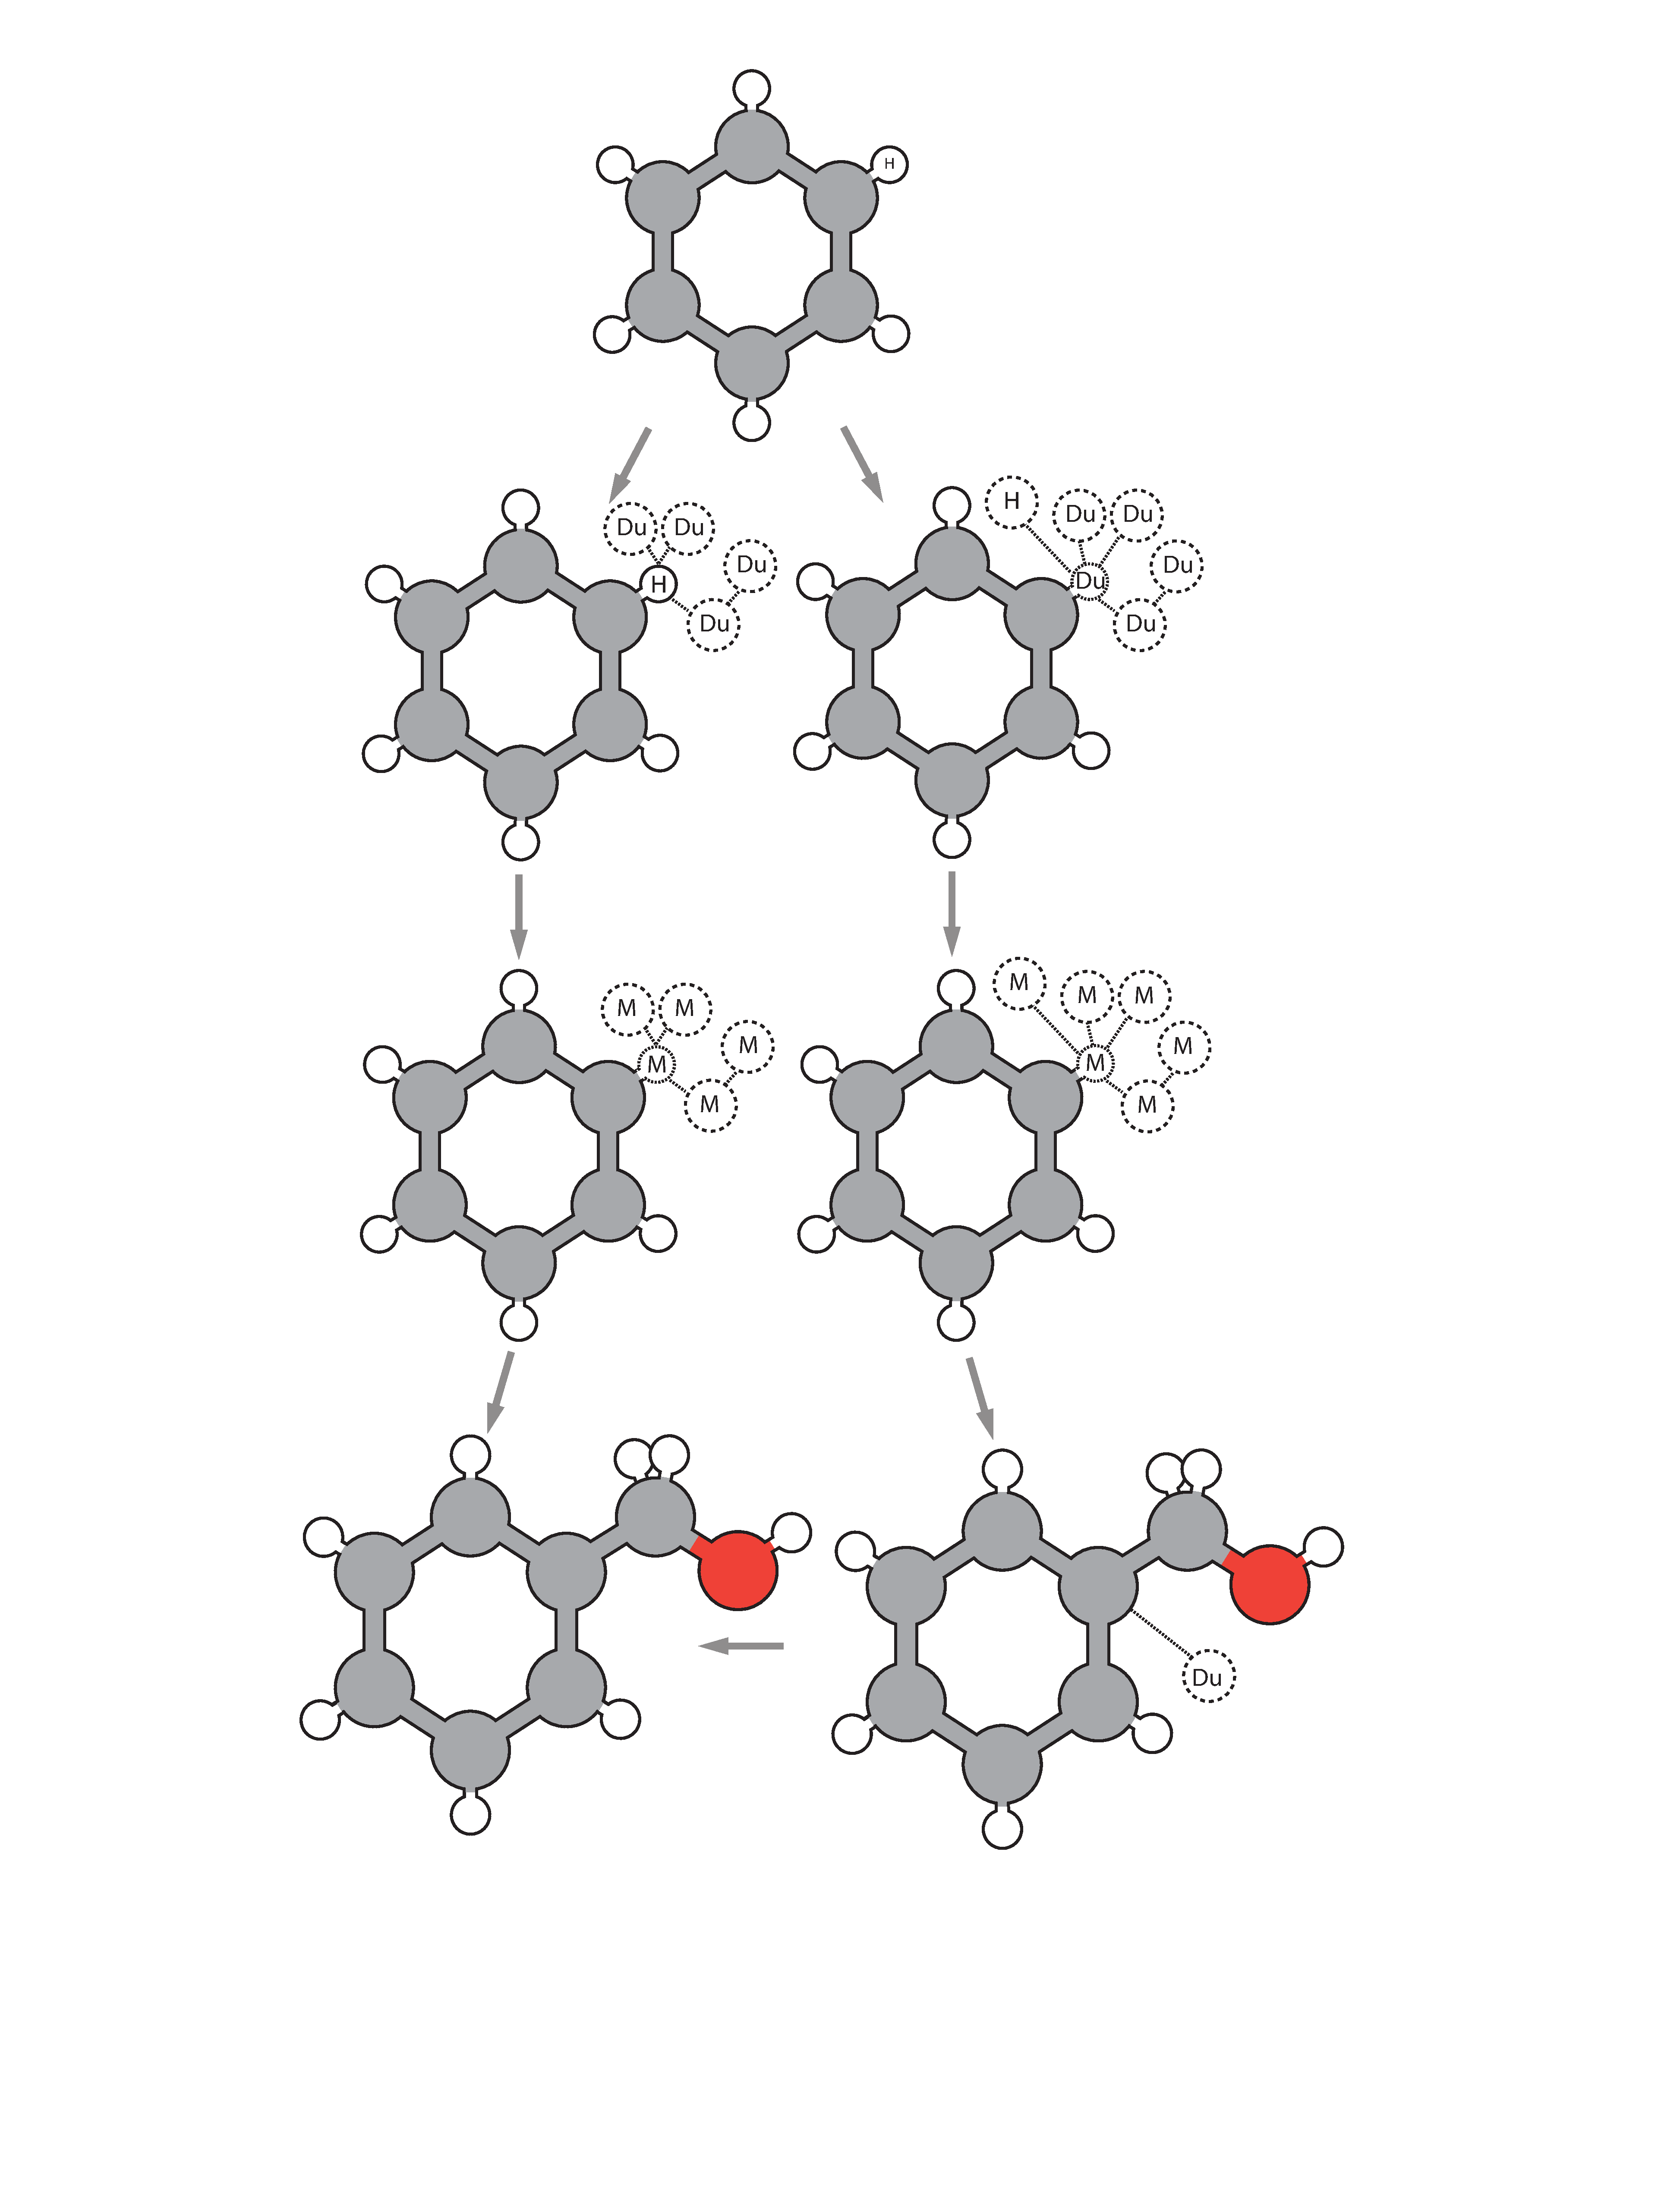
\includegraphics[width=0.95\columnwidth]{figures/fig3_topol/Figure.pdf}
    \caption{\textbf{Two common topologies for alchemical calculations: single and dual topology} \textbf{left}: A single topology uses softcore potentials to convert from one type of atom to an other. Dummy atoms (Du) are used when there is no corresponding maximum common substructure match between the two molecules for certain atoms. \textbf{right}: The dual topology does not convert one species to another, but only converts between Du atoms and an interacting species, but usually uses softcore potentials for this. The 'mixed' intermediate atoms are used in both dual and single topology approaches. Only the way the transformation occurs and the end states differ. Following the arrow along the left and right illustrate the differences.  Figure adapted from \url{http://www.alchemistry.org/wiki/Constructing_a_Pathway_of_Intermediate_States}}
    \label{fig:fig_topology}
\end{figure} 
Hybrid topology calculations have seen much less use but essentially consist of two absolute free energy calculations in opposite directions at the same time (turning one molecule off while turning the other on)~\cite{jiang2019computing}.
At present, the most widely used approaches, such as in Schr\"{o}dinger's FEP+~\cite{wang2015accurate,wang2019protein} and in BioSimSpace~\cite{hedges2019biosimspace} (for which calculations may be planned with Lead Optimization Mapper (LOMAP)~\cite{liu2013lead} seem to use single topology approaches, though some codes only support dual topology.
To our knowledge efficiency differences have not been thoroughly explored, though conventional wisdom suggests that fewer dummy atoms are better~\cite{liu2013lead,mobley2012perspective}.
%
\paragraph{Atom mapping}
Once a particular approach to the topology is selected, a crucial next step is to identify the common atoms which will not be perturbed.
Rigorously, this process comprises of a maximal common substructure (MCSS) search of the molecules involved to identify the common substructure -- though the parameters of the MCSS search will differ depending on whether single or dual topology calculations are planned.
Specifically, with a single topology approach in mind, atom types are allowed to change, so a permissive MCSS search can be done, whereas with dual topology a more strict search is required.
\begin{figure}[h!]
    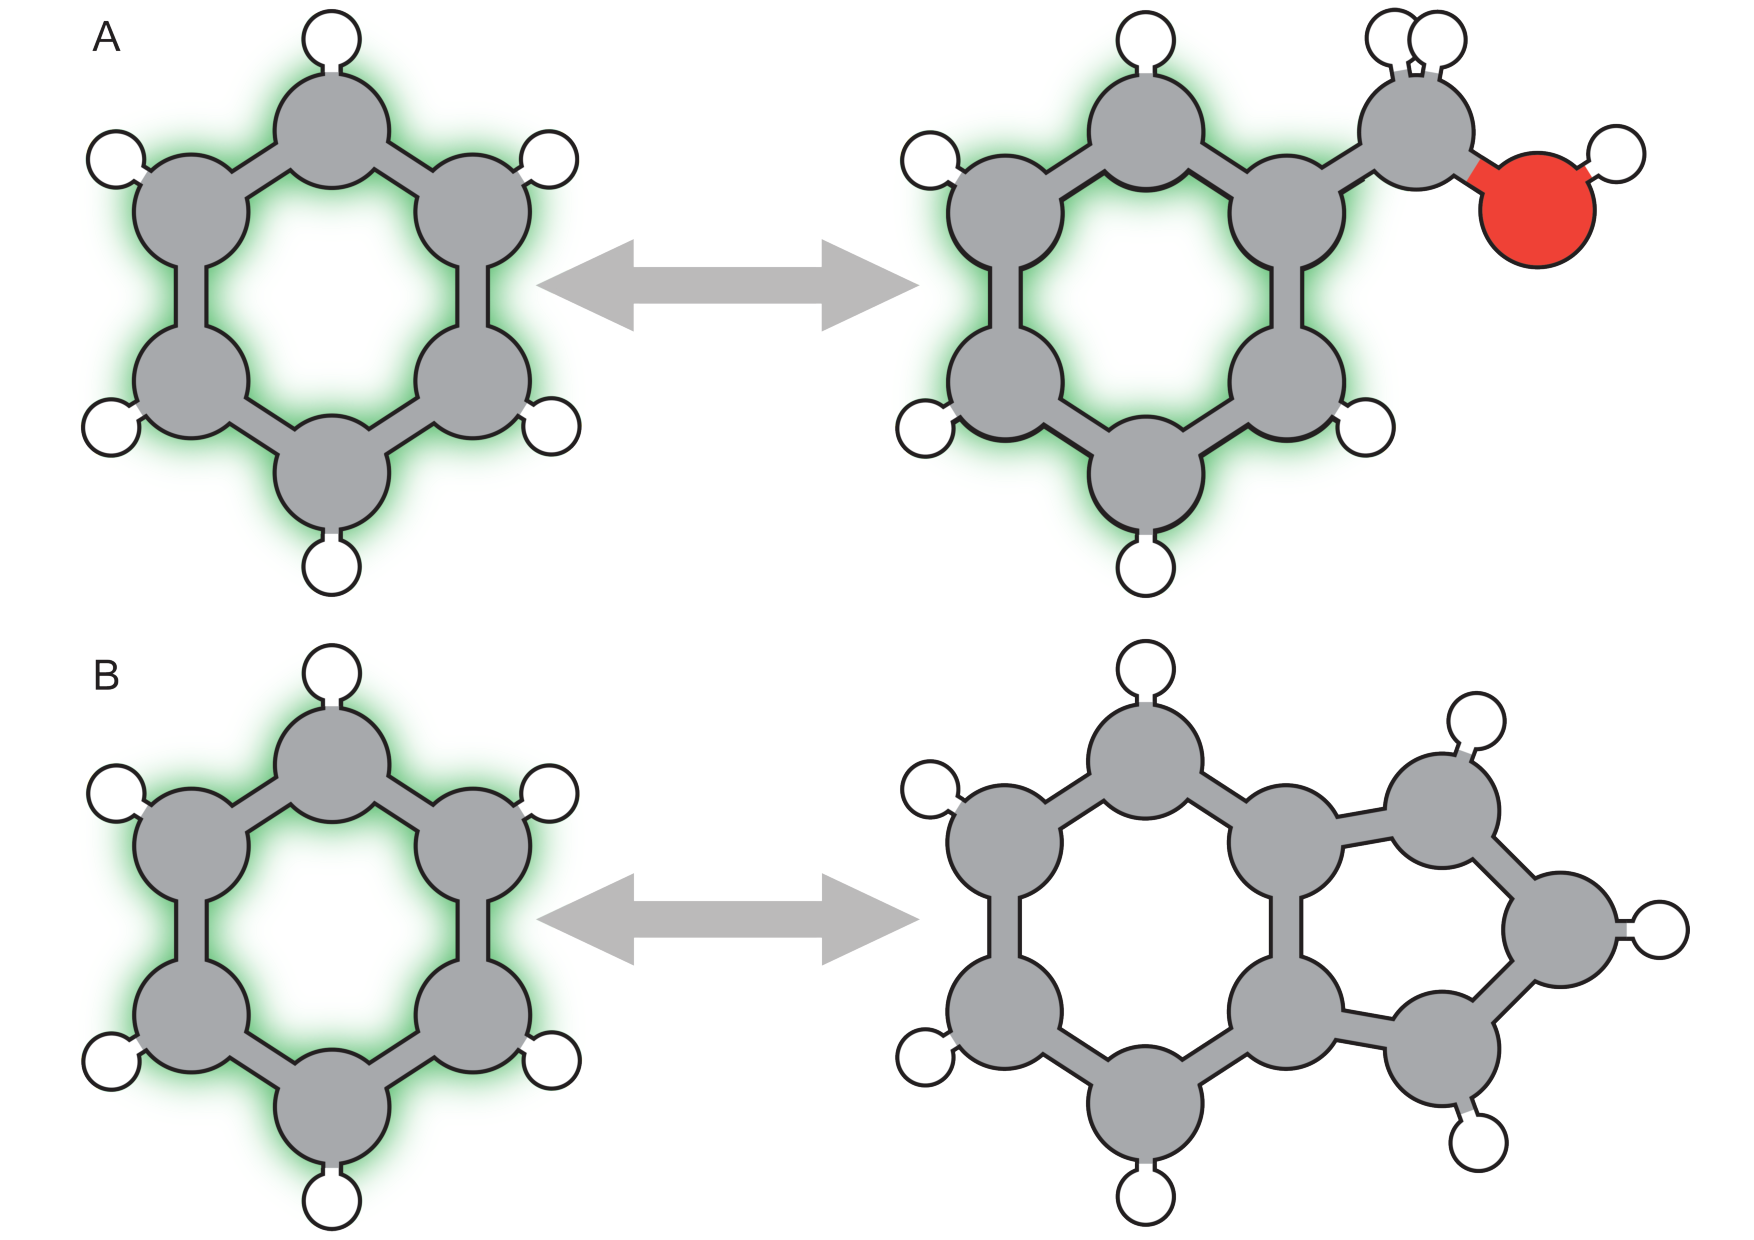
\includegraphics[width=0.95\linewidth]{figures/fig4_mcs/Figure.pdf}
    \caption{\textbf{Illustration of maximum common substructure matches} MCSS is shown in green for when (\textbf{A}) a restrictive MCSS match is used and in (\textbf{B}) ring breaking is allowed.}
    \label{fig:fig_mcss}
\end{figure} 
%
There are different tools that allow the generation of MCSS matches as well as single topology input. A large number of software can compute MCSS matches, some rely on RDKit~\cite{rdkit2019Dec}, such as LOMAP~\cite{liu2013lead} or FESetup~\cite{loeffler2015fesetup} and partially BioSimSpace~\cite{hedges2019biosimspace}, others such as fkckombu~\cite{kawabata20143d} are standalone tools. Schr\"{o}dinger's FEP+ planning tool is based on a version of LOMAP, and it also uses MCSS matching as well as 3D considerations to plan the network of single topology calculations between molecules~\cite{wang2015accurate}. 
%
MCSS searches can be relatively time consuming, so if the goal is to assess a library of ligands to identify promising pairs for relative calculations, it can be helpful to use faster approaches such as shape similarity to perform an initial assessment and then use MCSS only to identify final mappings for relative calculations~\cite{raymond2002maximum,klabunde2012mars,jones2009elucidating}.
%
The MCSS approach, though relatively standard, takes into account only topological similarity. It is possible that changes in binding mode could actually require a different choice of mapping, so in some cases mappings may need to be planned differently depending on 3D positioning of atoms in space.
%
Single topology relative calculations, and calculations based on substructure searches, only work if in fact the ligands share a common substructure, e.g. are part of a congeneric series, see Fig.~\ref{fig:fig_mcss}
If no common substructure is shared, then alternative dual or hybrid topology free energy calculations are needed, where one would co-localize a pair of compounds in a binding site, exclude their interactions with one another, and compute the relative binding free energy by turning one molecule on from being dummy atoms while turning the other off.
To our knowledge no general pipeline for such calculations yet exists and this would likely remain a research problem. Using an absolute style free energy calculation instead seems a more promising approach in such a case. 
%
\paragraph{Ring breaking and forming.} Relative free energy calculations for ring breaking and forming are particularly challenging/problematic (see Fig.~\ref{fig:fig_mcss} \textbf{B}), in part because relative calculations rely on the free energy contributions of dummy atoms canceling between different legs of the thermodynamic cycle, which may not be true whenever dummy atoms are involved in rings.
Some approaches have attempted to address this~\cite{clark2019relative} but a general solution is not yet in mainstream use.
%
\paragraph{Perturbation maps}
Based on the input ligand series a perturbation map or network can be planned. Recent heuristics have shown the more connected the perturbation network the better, however, there is a way to optimise network structure while minimising the number of perturbations that need to be computed minimising the resulting computational cost~\cite{yang2020optimal}. Sometimes the introduction of intermediates that are not part of the original congeneric series are essential to avoid ring breaking, or dealing with perturbations that would otherwise result in large numbers of atoms to be grown or disappearing. Some commercial tools have underlying good heuristic but may fail with complicated input, needing user validation in particular when dealing with chiral compounds. 
\begin{figure}[h!]
    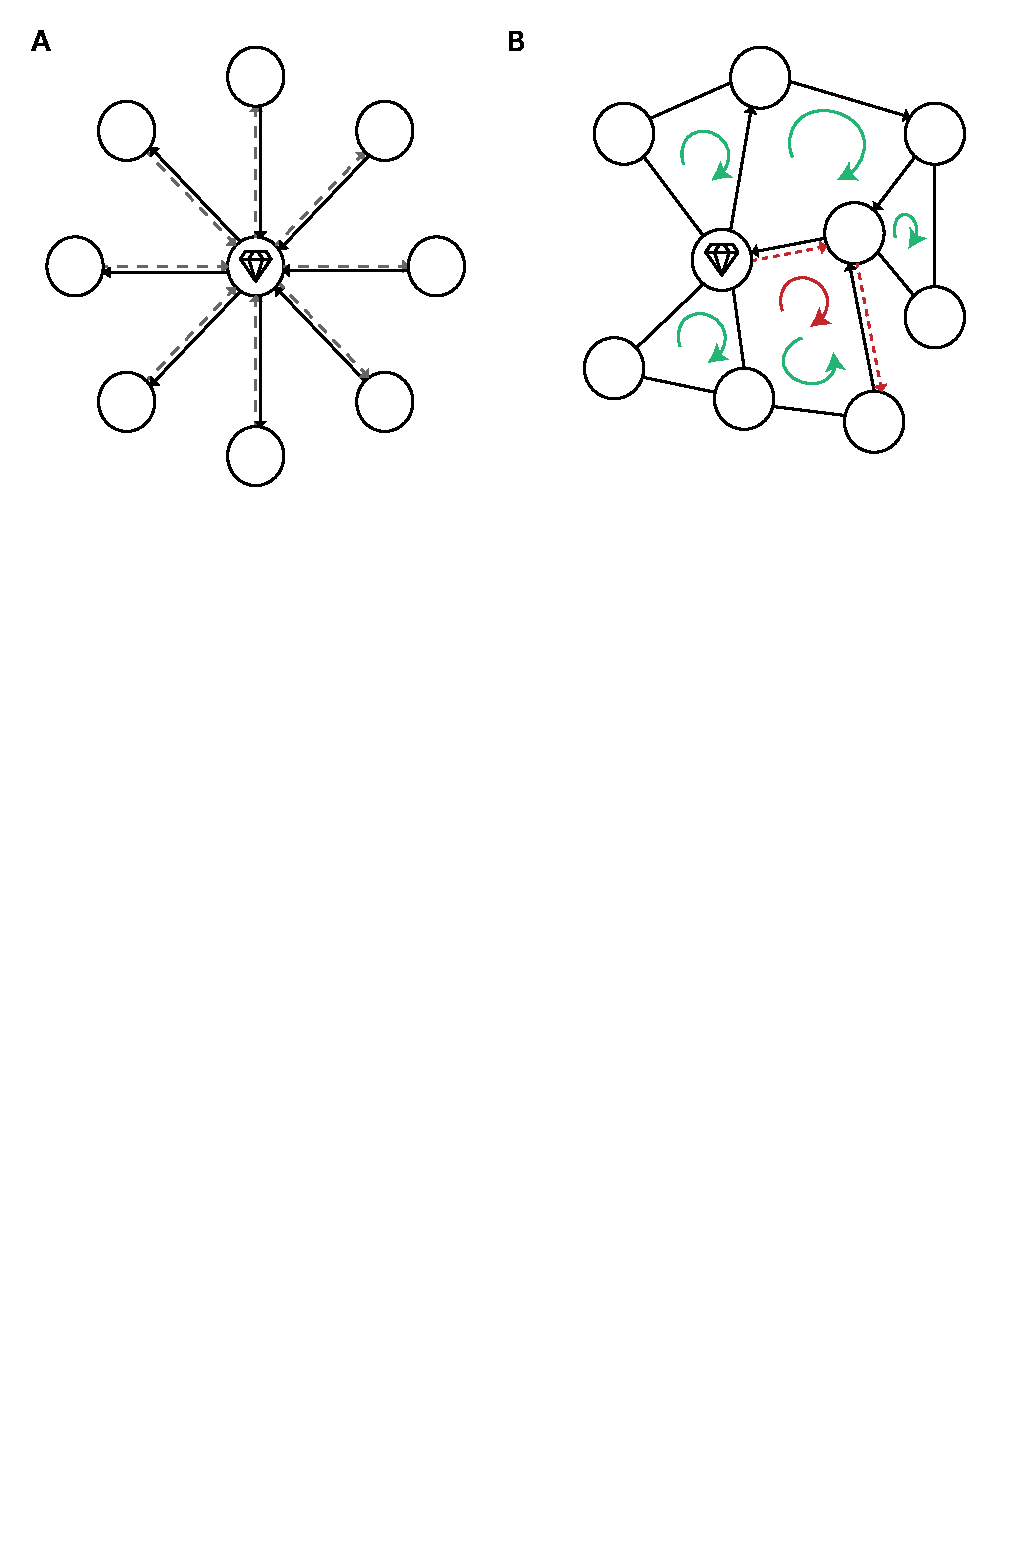
\includegraphics[width=0.95\columnwidth]{figures/fig6_types_of_networks/Figure.pdf}
    \caption{\textbf{Examples of perturbation networks} \textbf{A} Star shaped network with the crystal structure in the center. \textbf{B} Network with cycle closures (see more on this in Sec.~\ref{sec:are-they-good}). Arrows indicate the direction of the perturbation. Green cycles indicate good cycle closure, red poor cycle closure. The red arrow indicates a poorly converged simulation that would give rise to bad cycle closures. The diamond indicates the use of a crystal structure binding mode.}
    \label{fig:fig_types_of_networks}
\end{figure} 
In some cases, during the lead optimization stage, or if perturbations would be rather large a star shaped network as seen in Fig.~\ref{fig:fig_types_of_networks} (\textbf{A}) is used. However, adding redundancy into the network means that a better error analysis can be carried out, by looking at cycle closure errors as discussed in sec.~\ref{sec:are-they-good}, with an example given in Fig.~\ref{fig:fig_types_of_networks} (\textbf{B}).
%
Methods in experimental design have been applied to the construction of the perturbation maps. Yang et al.~\cite{yang2020optimal} optimized the perturbation map by selecting a fixed number of calculations from the pairwise perturbations so that the resulting set of calculations minimize the total variance. Xu~\cite{xu2019optimal} optimized the perturbation map by allocating different amounts of simulation time to different pairwise perturbations so as to minimize the total variance, given the total simulation time of all the perturbation calculations. Both approaches lead to substantial reduction in the statistical error of the estimated free energies.  
%
\paragraph{Constraints and relative free energy calculations}
One issue which requires particular care is the use of constraints.
Commonly, bonds involving hydrogen are constrained to a fixed length using algorithms such as SHAKE or LINCS, allowing the use of longer timesteps~\cite{krautler2001fast}.
However, in single topology relative free energy calculations, the atoms involved might be mutated to other atom types -- for example, in a mutation of methane to methanol, one hydrogen might become an oxygen atom.
Typical molecular dynamics engines are not set up to recognize this change, or at least not to correctly include contributions to the free energy from changing constraints/constraint length, so results for a transformation would usually be erroneous.
At present the most general solution to this problem is simply to avoid the use of constraints (and thus use a smaller timestep if necessary, usually of around 1 fs) in any relative free energy calculation involving a transformation of a constrained bond, as done by GROMACS. 
%
\subsubsection{Absolute free energy calculations must handle the standard state and use restraints}
\label{sec:standardstate-restraints}
%
\begin{figure}[h!]
    \includegraphics[width=0.95\linewidth]{figures/fig5_thermo_cyc_abs/Figure.pdf}
    \caption{\textbf{Thermodynamic cycle required for an aboslute free energy calculation -- absolute free energy of binding example} The fully interacting ligand in water (\textbf{A}), has its charges turned off to pass to \textbf{B} followed by turning of van der Waals terms, resulting in a non-interacting ligand in water in \textbf{C}. Restraints are used on the fully interacting ligand in the binding site of a protein or host molecule \textbf{D}. The next step is to turn off the charges again (\textbf{E}) followed by the van der Waals interactions resulting in a non-interacting complex state (\textbf{F}). Free energyes can be computed as $\Delta G_{bind} = (\Delta G^{\mathrm{elec}}_{\mathrm{solv}}+ \Delta G^{\mathrm{VdW}}_{\mathrm{solv}})-(\Delta G^{\mathrm{elec}}_{\mathrm{bound}}+ \Delta G^{\mathrm{VdW}}_{\mathrm{bound}}$).
    }
    \label{fig:fig_absolute_thermodynamic_cycle}
\end{figure}
%
Absolute free energy calculations involve completely removing the interactions between the ligand or solute and its environment, taking it to a non-interacting state that may or may not retain intramolecular non-bonded interactions.
This non-interacting state can then be shifted between environments (from the protein to water, or from one solution to another) without changing its free energy, and then interactions can be restored.
%
Absolute free energies are typically reported with respect to a specific reference or standard state, which effectively determines the arbitrary point at which the free energy is 0.
The role of the standard state is particularly evident with binding free energies, in which having a reference state allows us to obtain a well-defined partial molar free energy for the reaction
\begin{equation*}
\ce{AB <=> A + B}
\end{equation*}
through the well-known expression derived from the law of mass action
\begin{equation} \label{eq:DGfromKAB}
\Delta G = -RT ~ \ln \left( c^{\circ} K_{AB} \right)  = -RT ~ \ln\left( \frac{c^{\circ} C_{AB}}{C_A C_B} \right) ,
\end{equation}
where $R$ is the gas, $T$ is the temperature, $C_X$ is the equilibrium concentration of the chemical species $X$ in the reaction solvent, and the reference state concentration $c^{\circ}$ converts the binding constant $K_{AB}$ into a dimensionless quantity expressed in reference concentration units.
It should be noted that ignoring the term $c^{\circ}$ is equivalent to assuming a reference concentration of 1~D$^{-1}$, where D are the units used to express $K_{AB}$, and would thus cause the value of $\Delta G$ to vary with the choice of the units.
Typically, it is convenient to define a standard state at a constant pressure of 1~atm and where each chemical species (i.e., A, B, and AB) in the reaction solvent has a concentration of $c^{\circ}$~=~1~M~=~1~molecule/1660~\r{A}$^3$ but do not interact with other molecules of A, B, or AB.
%
\paragraph{Handling the standard state in absolute free energy calculations.}
For solvation free energy calculations, handling the standard state is typically straightforward, and treating it correctly simply means ensuring that the non-interacting solute is taken to the same (or equivalent) final reference state in both environments, e.g. that the transformation involves a 1 M to 1 M equivalent transfer free energy (where the non-interacting solute still occupies essentially the same volume as the solute in the interacting system).
So typically in such cases no special care is required to ensure the correct standard state, as long as the \emph{experimental} data being analyzed uses the same standard state and if it does not, a simple entropic correction is needed.
%
However, for binding the situation is much more complex and requires special care.
Experimental absolute binding free energies are reported relative to a specific reference state -- a 1 M standard state -- which must also be used in calculations.
In practice, this has implications for how the calculations are done, as the reference concentration must enter the thermodynamic cycle employed, see an example of such a thermodynamic cycle in Fig.~\ref{fig:fig_absolute_thermodynamic_cycle}.
%
Typically, to deal with both practical sampling issues and the standard state issue, restraints are employed in absolute binding free energy calculations to keep the ligand in a well defined volume as its interactions with the system are removed~\cite{gilson1997statisticalthermodynamic}.
This solves two problems.
First, if the ligand were not kept in a well-defined region, as its interactions were removed it might wander the system, perhaps quite slowly, and only inadequately sample the non-interacting or weakly interacting state -- yet adequate sampling of these states might be required for convergence.
So for practical purposes, the use of restraints can dramatically improve sampling as interactions are weakened and removed.
Second, if the ligand is not kept in a well-defined region then it is hard to determine how to link a computed binding free energy to the correct 1 M standard state.
In contrast, with restraints, the free energy of releasing the restrained ligand to a 1 M standard state can be computed analytically or numerically by solving the relevant integral, allowing the standard state to enter the thermodynamic cycle.
%
\paragraph{Several choices of restraints are possible.}
In practice, a variety of types of restraints are common, from simple harmonic distance restraints between the ligand and the protein~\cite{mobley2006use}, to flat-bottom restraints which work similarly but only exert a force if the ligand leaves a specific region~\cite{chen2007can}.
%
Alternatively, a set of restraints proposed by Boresch have also commonly been employed, where all six rigid-body degrees of freedom governing the orientation of the ligand relative to the receptor are restrained~\cite{boresch2003absolutea, leitgeb2005alchemical}.
Further restraints, such as on the overall ligand RMSD have also been used~\cite{woo2005calculation}.
%
In principle, all of these forms will yield correct binding free energies in the limit of adequate sampling (if their effects and connection to the standard state are correctly handled) but they have different strengths and weaknesses.
For example, with more involved restraints, sampling at intermediate $\lambda$ values will usually not need to be as extensive but more computational effort must go to computing the restraining free energy.
Additionally, such restraints would typically keep the ligand from exploring alternative binding modes, which may be undesirable with Hamiltonian $\lambda$ exchange or expanded ensemble techniques where allowing the ligand to exchange binding modes when it is non-interacting could provide sampling benefits~\cite{wang2013identifying}.
Concretely, flat-bottom restraints might allow a ligand to explore multiple binding sites, harmonic restraints multiple binding modes within a site, and Boresch restraints a single binding mode within a single site.
See additional discussion of the possibility of multiple binding modes in Sec.~\ref{sec:multiple_binding_modes} below.
%
Many choices of restraints involve selecting reference atoms.
Again, in principle this choice is unimportant given adequate simulation time but practical considerations may be important.
The choice is likely especially important with Boresch-style restraints, where some relative placements of reference atoms are likely to be numerically unstable; additionally, ligand reference atoms should likely be in a part of the molecule which defines the binding orientation well, rather than in a floppy solvent-exposed tail, for example.
\todo[inline, color={blue!20}]{DLM: Get input from JDC on what they've learned about these.}
\todo[inline, color={blue!20}]{DLM: Clarify terminology: Double decoupling, etc. See Feature Box below.}
%
%
\subsection{Absolute and relative calculations must deal with some of the same issues}
\subsubsection{Structural definition of the bound state and weak binders}
\todo[inline, color={green!20}]{ASJM: This a bit waffly. What are the recommendations, of how to setup these restraints?}
In binding free energy calculations, extra care should be taken when simulating the bound state, especially when dealing with weak binders and absolute free energy calculations in combination with enhanced sampling techniques.
In principle, only configurations of the receptor-ligand complex that we consider "bound" should be sampled from the bound state, and, in atomistic simulations, this requires to establish a structural definition of the bound state.
In practice, the simulation of the bound state starts with the ligand already placed in the binding site and relies on kinetic trapping to maintain a bound complex.
However, this strategy may not be sufficient if the complex dissociation rate is high or if methodologies such as Hamiltonian replica exchange~\cite{bitetti-putzer2003generalized} and expanded ensemble~\cite{chodera2011replica} are employed in absolute free energy calculations to enhance sampling since, in both cases, the ligand may find a way out of the binding site on timescales that are achievable by modern MD simulations.
A solution commonly adopted in these cases is the use of one or more restraints making the unbound configurations energetically unfavorable through the addition of extra terms in the potential function.
In practice, even with restraints, it is not always trivial to force a molecular dynamics simulation to explore a restricted region of the configurational space with a complicated geometry such as a binding site.
If the ligand is a tight binder\todo[inline, color={red!40}]{AR: Should we give an order of magnitude to define a tight and a weak binder? ASJSM: Yes!}, it is usually safe to employ a restraint that allows some of the unbound configurations to be sampled since they generally contribute negligibly to the partition function (i.e., they have a relatively small Boltzmann weight) as long as the sampled volume is not so large that their cumulative contribution becomes significant.
However, this is more problematic when dealing with weak binders as the unbound configurations can have a non-negligible Boltzmann weight, and their binding affinity can exhibit a significant dependency on the restraint type and parameters that are used to determine the sampled volume~\cite{}.
Moreover, it should be noted that the additional potential energy terms used to model the restraints can introduce a bias in the predicted free energy.
The bias can be removed at the analysis stage through reweighting techniques, but this procedure can increase the statistical uncertainty of the binding free energy estimate when the restraints are so strong that the overlap with the reweighted state is diminished~\cite{}.
%
Finally, it is useful to keep in mind that, for a meaningful comparison between computational predictions and experimental measurements, the definition of the bound state should be consistent.
In particular, this means that the signal used by the experimental methodology to determine the fraction of bound complexes in solution should in principle reflect the population of complexes in the bound state as defined in the calculation.
%
\subsubsection{Changes in net charge can be challenging/problematic.}
If the net charge of the system will change as the alchemical calculation progresses, this can pose major challenges.
Specifically, finite-size effects can introduce profound artifacts into computed binding free energies~\cite{}, in part because typical schemes for long-range electrostatics (including PME and reaction field) do not handle free energy contributions from such changes effectively or as they would be handled in a hypothetical macroscopic bulk solution~\cite{}.
%
There are two main potential solutions to avoid artifacts due to changes in net charge: Correcting for the introduced artifacts, or avoiding changing the net charge.
%
Many relative free energy planning tools have been set up to avoid changing the net charge of the systems considered, including LOMAP~\cite{liu2013lead} and Schr\"{o}dinger's FEP+~\cite{wang2015accurate}. Absolute free energy calculations can also potentially avoid changing the charge of the system by making a charge perturbation of equal and opposite sign elsewhere in the system; for example, as a charged ligand is removed, a charged counterion of opposite sign could also be removed, or one of the same sign could be inserted. This is sometimes referred to as an "alchemical ion" approach for dealing with the needed charge change, and is also employed by the Yank free energy package~\cite{wang2013identifying}.
Charge corrections have also been explored, and are potentially a viable solution to this problem~\cite{mey2018impact} where artifacts introduced by finite-size effects are corrected numerically.
~\cite{chen2018accurate}. However, application of such corrections typically remains less common than the use of a co-alchemical ion.
%
When free energy calculations \emph{do} need to change the charge of a ligand or solute, the literature does not yet seem to indicate what approach should be preferable, so considerable care should be taken.
We are not yet aware of a careful comparison of charge corrections versus other approaches such as decoupling an ion at the same time, so in our view the issue of proper handling of charge mutations in the context of alchemical calculations remains a research problem.
%
\subsubsection{The importance of the alchemical pathway
\label{sec:important_path}}
\todo[inline, color={red!40}]{LNN: write common principles alchemical path choice. MRS: mostly wrote this, LNN can comment on it. LNN: LGTM}
\todo[inline, color={red!40}]{AR: write absolute-specific section on  alchemical path choice}
\todo[inline, color={red!40}]{BA: write relative-specific section on  alchemical path choice}

\begin{figure}
    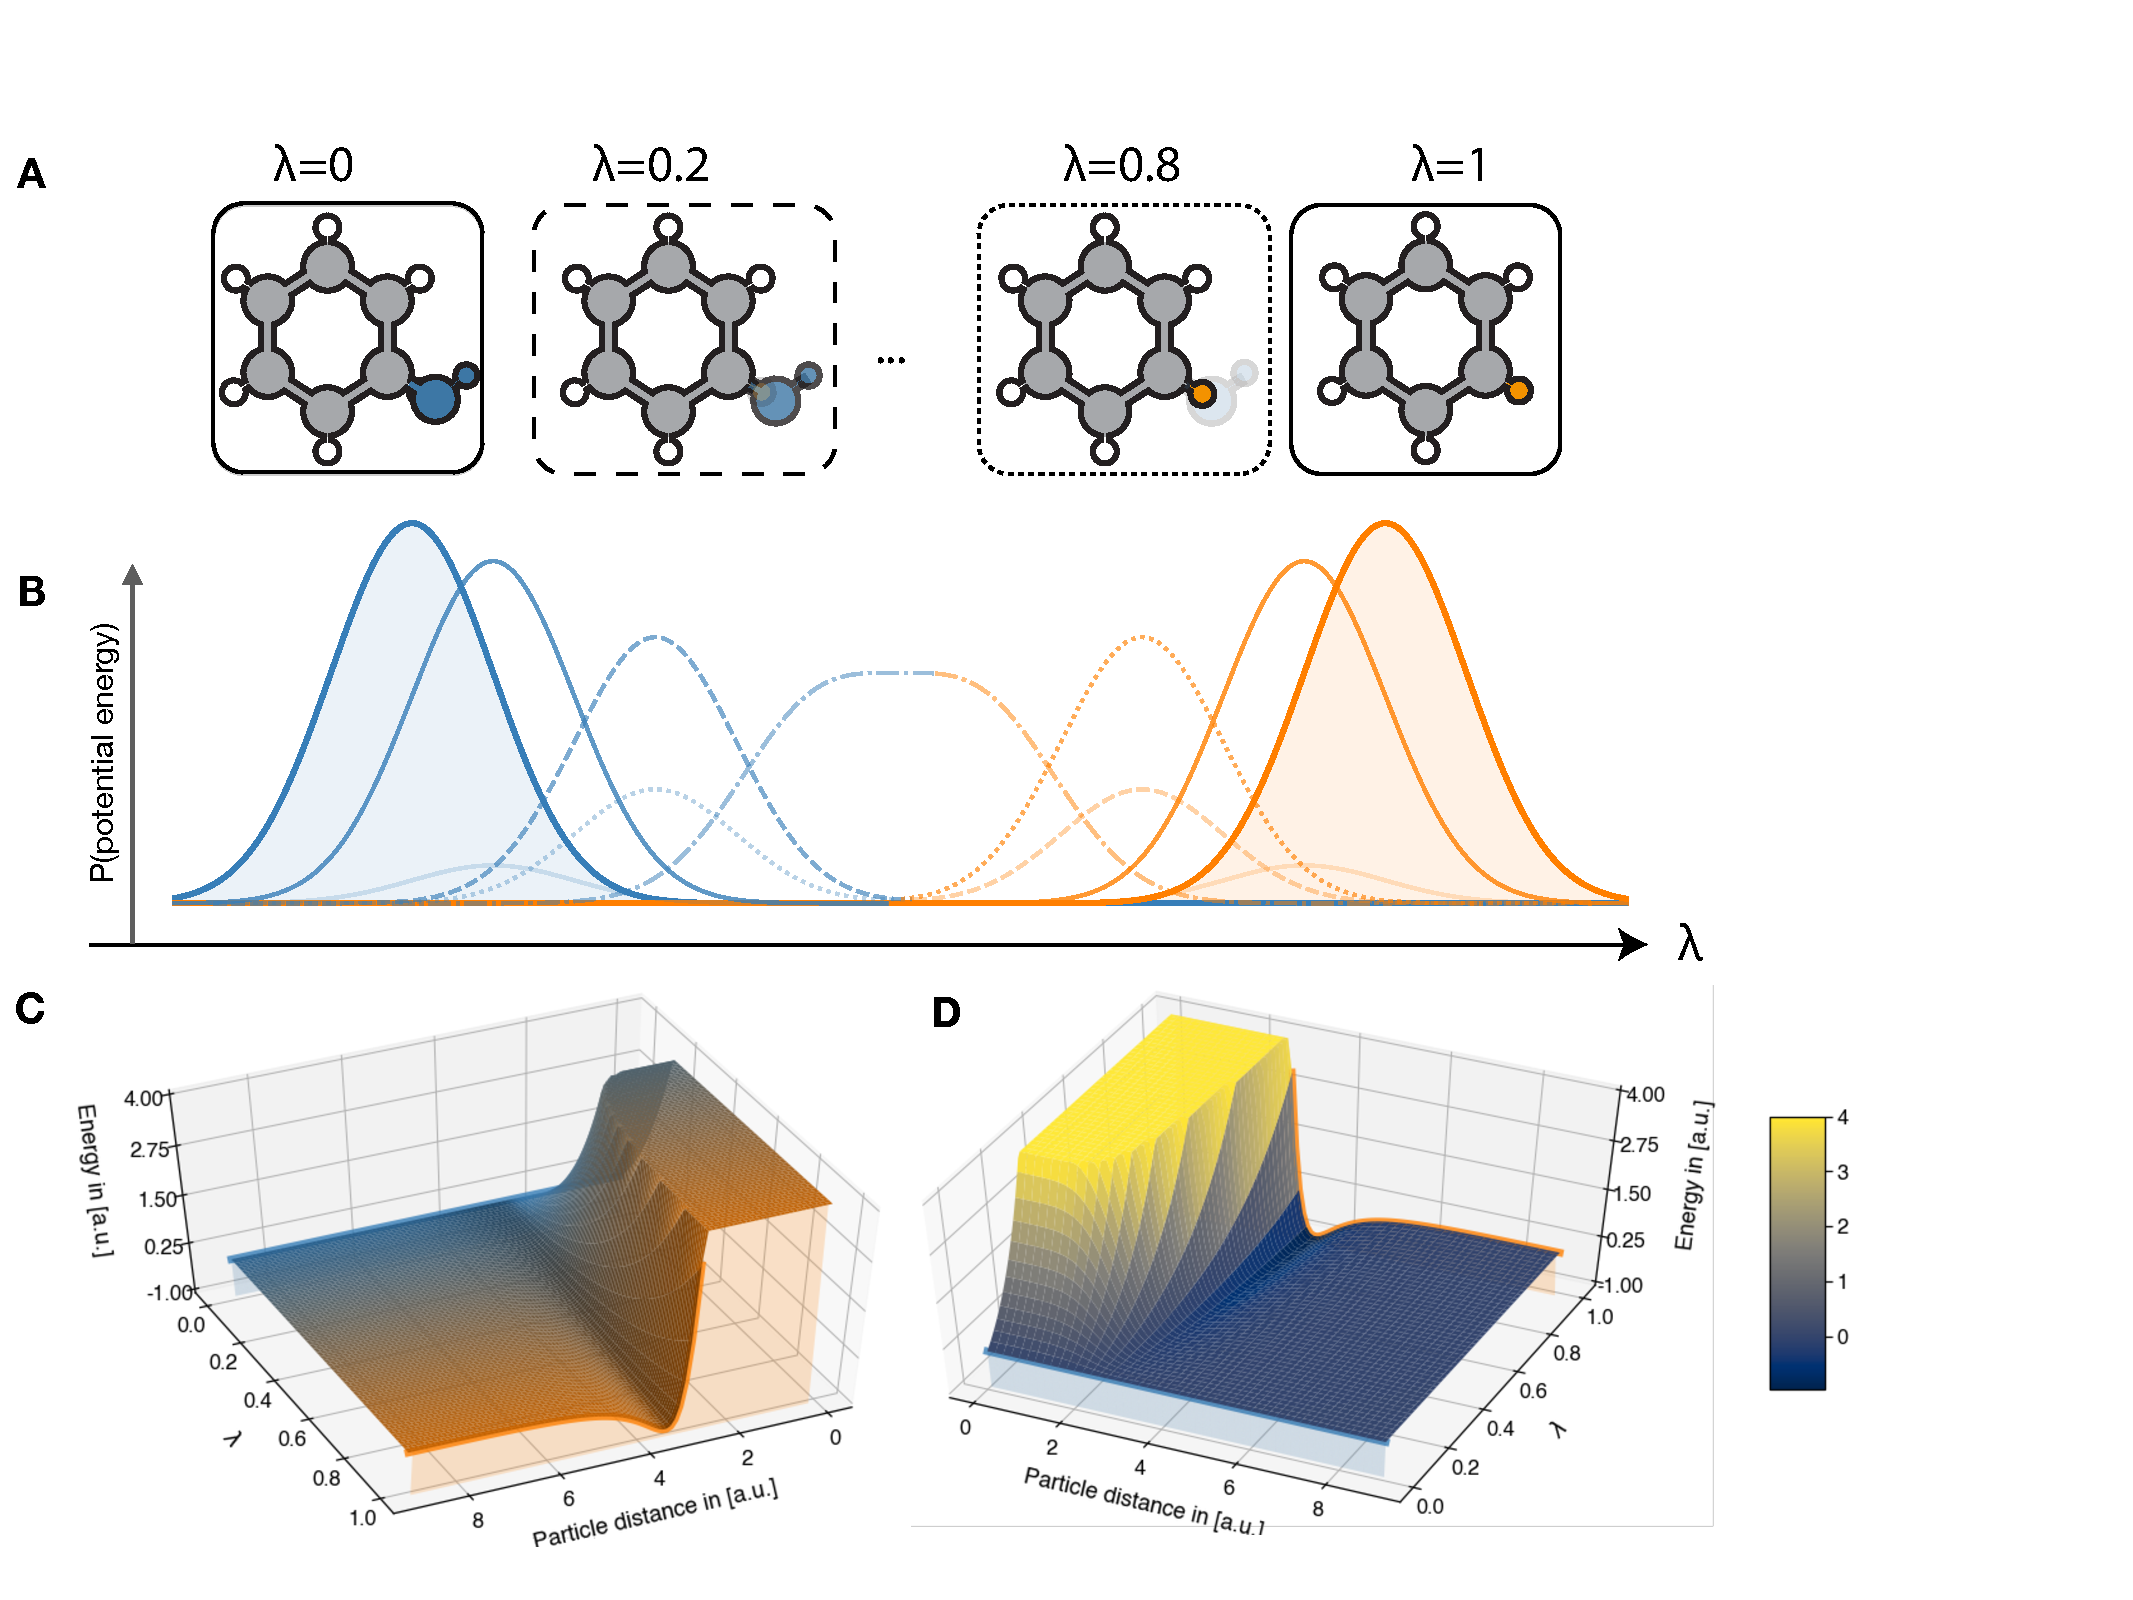
\includegraphics[width=0.95\linewidth]{figures/fig7_what_is_lam/Figure.pdf}
    \caption{Alchemical intermediates are createtd by making the potential energy depend on a an additional variable $\lambda$ that interpolates between the chemical endpoints. In \textbf{A}, at $\lambda=0$ the molecule is a fully interacting phenol and at $\lambda=1$,  a fully interacting benzene.  \textbf{B} shows an illustration of the probability distribution of the potential energies as the switching function takes values of $\lambda=0$ to $\lambda=1$, intermediates are required for a sufficient overlap in potential energies to estimate a free energy difference between $\lambda=0$ and $\lambda=1$.
    One of the most efficient families of intermediate pathways  are softcore potentials, whose shape is illustrated in \textbf{C} with dependence on $\lambda$ and \textbf{D} with dependence on the potential energy. Note how when $\lambda$ approaches 0, the energy smoothly approaches zero at all $r$, a necessary requirement for efficient calculations.  }
    \label{fig:fig_what_is_lambda}
\end{figure}
%
Both absolute and relative calculations must choose an alchemical pathway connecting initial and final states. In principle, because of the path independence of the free energy, any arbitrary pathway will give the correct free energy change, but the choice of pathway will greatly affect the efficiency of the calculations. 
Some choices are particularly crucial -- for example, transformations involving insertions or deletions of atoms should employ a soft-core potential path for Lennard-Jones or other interactions with repulsive interactions that go to infinite energy at small radius~\cite{beutler1994avoiding, beutler1994molecular,gapsys2012new}.
%
The key consideration for choosing alchemical pathways is that the intermediate states that a given pathway produces should sample configurational ensembles that change as slowly as possible as $\lambda$ changes, while still managing to go from the initial state to the final state as $\lambda$ goes from 0 to 1.
%
Another way of stating this is that intermediate states should sample molecular configurations that are as similar as possible to their neighboring states. The more similar the configurations are between intermediate states, the lower the statistical uncertainty is in the estimate of free energy between intervals. This can be proven directly from the BAR and MBAR formulas~\cite{bennett1976efficient,klimovich2015guidelines}, though the exact same principles apply for TI. For a 'good' path to work sufficient overlap between pontential energies is required. Fig.~\ref{fig:fig_what_is_lambda} \textbf{A} and \textb{B} try to illustrate this. Fig.~\ref{fig:fig_what_is_lambda} \textbf{A} shows in a pictorial way a soft-core potential can be applied across different $\lamda$s. Fig.~\ref{fig:fig_what_is_lambda} \textbf{B} illustrates the potential energy distributions at the different $\lambda$ intermediates, with sufficient overlap between neighboring $\lambda$ states to ensure that reweighting estimators such as MBAR can be used for analysis (see Sec.\ref{subsec:estimators}). The actual transformation is best handled with soft-core potentials of the form shown in Fig.\ref{fig:fig_what_is_lambda} \textbf{C} and \textbf{B}, with more details given below. 
%
So how do we adjust the potentials between the two end states based on $\lambda$? The simplest possible alchemical pathway is a \textit{linear} pathway:
%
\begin{equation}
U(\vec{q},\lambda) = \lambda U_0(\vec{q}) + (1-\lambda)U_1(\vec{q})   
\end{equation}
%
so-called because the dependence on $\lambda$ is linear. This clearly satisfies the basic requirement that it gives the initial endpoint potential energy $U_0(\vec{q})$ when $\lambda=0$ and final endpoint energy $U_1(\vec{q})$ when $\lambda=1$. 
%
For many energy terms, \textit{as long as a repulsive core remains on}, this is a very good approach. For example, it can be shown that if van der Waals repulsions are left on, then the linear approach is very nearly the optimal path possible for changing, removing, or inserting the electrostatic energy terms, with the path being within about 10--20\% of the minimum possible uncertainty~\cite{naden2015linear} for a fixed amount of simulation, as well as being nearly optimally efficient for van der Waals attractive terms with repulsion terms turned on~\cite{naden2014linear}. Although we are not aware of any quantitative tests for dipolar or higher multipole terms, theoretically it should behave equally well for those systems.
%
However, this approach ends up being terrible for removing or adding repulsive potentials that go to infinity quickly at or near the origin. One way to look at this is to examine how low $\lambda$ values must go to reduce the energy at $0.5\sigma$ (the atomic size parameter) down to 1 $k_BT$, where thermal fluctuations make it possible for other atomic sites to penetrate routinely that deep. If we are trying go from a particle being present, and desire to make it disappear alchemically, then if the repulsive terms is of the form $\epsilon\frac{\sigma}{r}^{12}$, then if $\epsilon$ was 1 $K_BT$ at the temperature of interest, and we start with the particle present, then solving for $(1-\lambda)(1 kB_T)\frac{\sigma}{\frac{1}{2}\sigma}) = 1 k_B T$ we get $\lambda = 1-2^{-12} \sim 0.999976$. So we have gone virtually all the way to the end of the transformation, there's still an impenetrable post in the middle of our simulation! This is not very much like the desired final state of no interactions between the particle and its environment. We can play around with a few ways of modifying this, like simulating many more intermediate states near $\lambda=1$. Various analyses have shown that this is not a very good strategy, however~\cite{pham2011identifying, beutler1994avoiding, zacharias1994separationshifted, blondel2004ensemble, gapsys2012new}.
%
What we need instead is some sort of function that smoothly gets rid of this infinity. A large number of scheme have been tried~\cite{beutler1994avoiding, zacharias1994separationshifted, blondel2004ensemble, pham2011identifying, pham2012optimal, naden2014linear, donnini2005molecular}, but the most common strategy that appears to be the best practices is to use a "soft-core" potential, of the form:
%
\begin{equation}
    U(\vec{r_{ij}},\lambda) = 4\epsilon_{ij} \lambda \left(\frac{1}{(\alpha(1-\lambda) + (r_{ij}/\sigma_{ij})^6)^2} +  \frac{1}{\alpha(1-\lambda) + (r_{ij}/\sigma_{ij})^6}\right)\label{eq:softcore}
\end{equation}
Where $r_{ij}$ is the distance between two particles $i$ and $j$, $\epsilon_{ij}$ and $\sigma_{ij}$ are the Lennard-Jones parameters corresponding to the interaction between particles $i$ and $j$, and $\alpha$ is a constant (0.5 is optimal for the functional form shown above).  This functional form has exactly the property we are looking for: it recovers the Lennard-Jones potential when $\lambda=1$, and the other endpoint ($\lambda=0$), it is exactly zero for all $r_{ij}$ everywhere, and as $\lambda$ goes to zero, the  $\alpha(1-\lambda)$ term lowers the infinite energy in the core.  There are several different variants of the same functional form~\cite{zacharias1994separationshifted, beutler1994avoiding,pham2011identifying}, but the one in given in eq.~\ref{eq:softcore} is easy to understand and implement and fairly numerically stable. This functional form is shown in parts \textbf{C} and \textbf{D} of Fig.~\ref{fig:fig_what_is_lambda}.
It has been shown that more complicated forms are not significantly more efficient than eq.~\cite{pham2012optimal}.  We recommend using the softcore potential given in eq.~\cite{eq:softcore}, unless there is a compelling reason otherwise. Using a similar equation to eq.~\cite{eq:softcore} may be acceptable in most circumstances if that is what is supported in your chosen software. However, if you are inserting or removing entire atomic sites, we heavily recommend against using the linear approach; it will be very difficult to get correct results. 
%
We have discussed optimal ways of disappearing or appearing Lennard-Jones interaction sites and turning on and off electrostatics terms. What about performing both transformations at the same time? We can't turn off the electrostatics linearly at the same time we turn off the Lennard-Jones terms, as it would leave infinitely large attractive and repulsive electrostatic terms "bare" at small $\lambda$, resulting in the simulation crashing. It \textit{is} possible to apply the same soft core approach to the Coulomb interaction, but it turns out to be somewhat difficult to turn off two soft-core terms simultaneously~\cite{steinbrecher2011softcore}. We therefore recommend performing the transformations in sequence; first, turning off all electrostatics for atoms that must be removed, inserting and removing Lennard-Jones sites (both the insertion and removal can be done simultaneously), and then turning electrostatics for the introduced particles on. However, If there are no removals or introduction to atomic sites, then it is reasonable to change all interactions linearly.  
%
Other issues, such as whether absolute calculations should retain or remove intramolecular non-bonded interactions, may be less critical and recommendations differ among studies in the literature~\cite{}, and reasonable efficiency can be often obtained with either choice even if some are somewhat better or worse than others. Our recommendation is to leave the intramolecular interactions on during the transformation for simplicity if there are no other known issues with this approach.  The key thing to watch out for is whether the total potential energy, and therefore the intermediate ensembles sampled, change smoothly from beginning to end. If a configurational phase transition is noted in the process (like substantial dihedral rearrangement), then other steps must be taken, perhaps including modifying intramolecular interactions~\cite{???}. These problems can be diagnosed by noticing lack of configuration space overlap between different simulations (see section~\ref{sec:are-they-good})" 
%
Relative calculations introduce additional choices, including whether to define explicit intermediate states~\cite{} or leave these implicitly defined by the code~\cite{}.
Typically in single topology relative calculations it proves most efficient to first remove electrostatic interactions of any atoms which will be deleted, then modify other non-bonded interactions, then restore electrostatic interactions of any atoms which are being inserted.
Other schemes, such as simultaneously changing electrostatic and Lennard-Jones interactions, even with electrostatic ``soft-core'' potentials~\cite{steinbrecher2007nonlinear}, in our experience typically introduce errors and/or instabilities or are at least unreliable.
It is expected that similar considerations will apply to dualtopology calculations, and the principle of first removing electrostatics and then removing steric interactions will likely serve well.
%
A key additional consideration in choosing the alchemical pathway is the choice of spacing of intermediate states.
The spacing depends to some extent on the choice of analysis method, though states should essentially be spaced equidistant in the relevant thermodynamic length~\cite{crooks2007measuringa, sivak2012thermodynamic}.
For BAR/MBAR techniques this means that spacings should typically be equal in [what, variance? ref].
Some schemes to adaptively optimize the spacing of intermediate states based on initial exploratory simulations have been proposed~\cite{}.
%
An example of this approach for relative binding free energy calculations includes saving configurations from short 10 picosecond simulations starting at $\lambda_0$, and evaluating changes in the standard error of mean (SEM) in $\frac{dU}{d\lambda}$ as reevaluated at new values of $\lambda$, starting with a step size of 0.01 up to a predetermined threshold.
This threshold can be empirically defined as the number of atoms being inserted or deleted in the simulation / 100.
If the absolute value of the difference in SEM is below the defined threshold, then the change in $\lambda$ for re-evaluation of SEM in $\frac{dU}{d\lambda}$ is defined by the current difference in SEM from the threshold divided by the derivative of the SEM with respect to $\lambda$.
%
\subsubsection{What different sampling schemes exist and which one should I use?}
\label{sec:sampling_schemes}
With all alchemical simulations having the requirement of sampling from different sets of $\lambda$ states in common, different approaches have been designed to achieve this. Fig.~\ref{fig:fig_sampling_scheme} illustrates the four most common schemes used. The simplest approach is defining a set of fixed replicas each representing a different $\lambda$ value that run independent simulations at each of the intermediate $\lambda$ values, see Fig.~\ref{fig:fig_sampling_scheme}(\textbf{A}). This type of scheme is currently used for AMBER TI calculations~\cite{song2019} and for Siremol/Openmm~\cite{}. A slightly more complex approach is allowing replica mixing, meaning that each independent $\lambda$ simulation is attempted to be exchanged with a neighboring $\lambda$ replica. This is based on ideas of Monte Carlo simulations of spin glasses by Swendsen and Wang~\cite{swendsen1986replica}. Using a Metropolis Hastings based acceptance criterion for exchanges means that the generated ensemble of all replicas is still sampling from the Boltzmann distribution and has been used in many different contexts for molecular simulations~\cite{sugita2000multidimensionala,sugita1999replicaexchangea, woods2003developmenta, jiang2010free}. The basic idea of the replica exchange scheme is shown in Fig.~\ref{fig:fig_sampling_scheme}(\textbf{B}). It is supported in various software packages that provide alchemical implementations, such as GROMACS~\cite{aldeghi2015accurate}, FEP+~\cite{wang2015accurate}, and NAMD~\cite{jiang2019computing}. A third approach borrows ideas from simulated tempering~\cite{marinari1992simulateda}. In this scheme a single replica rapidly explores all of $\lambda$ space by optimally working out weights that allow switching between different intermediate $\lambda$ values, as seen in Fig.~\ref{fig:fig_sampling_scheme}(\textbf{C}) and also referred to as self adjusted mixture sampling~\cite{lyubartsev1992newa, li2007simulated, tan2017optimally} and while promising, has so far only been supported in OpenMM Tools~\cite{andrearizzi2019choderalab}. The last approach available in conjunction with GROMACS makes use of non-equilibrium simulations~\cite{aldeghi2018accurate}. In this approach, only end state $\lambda$ replicas ($\lambda$=0, $\lambda=1$) are simulated at equilibrium intermediate information is generated from non-equilibrium simulations. A schematic of this approach is shown in Fig.~\ref{fig:fig_sampling_scheme} \textbf{D}. 

\begin{figure}
    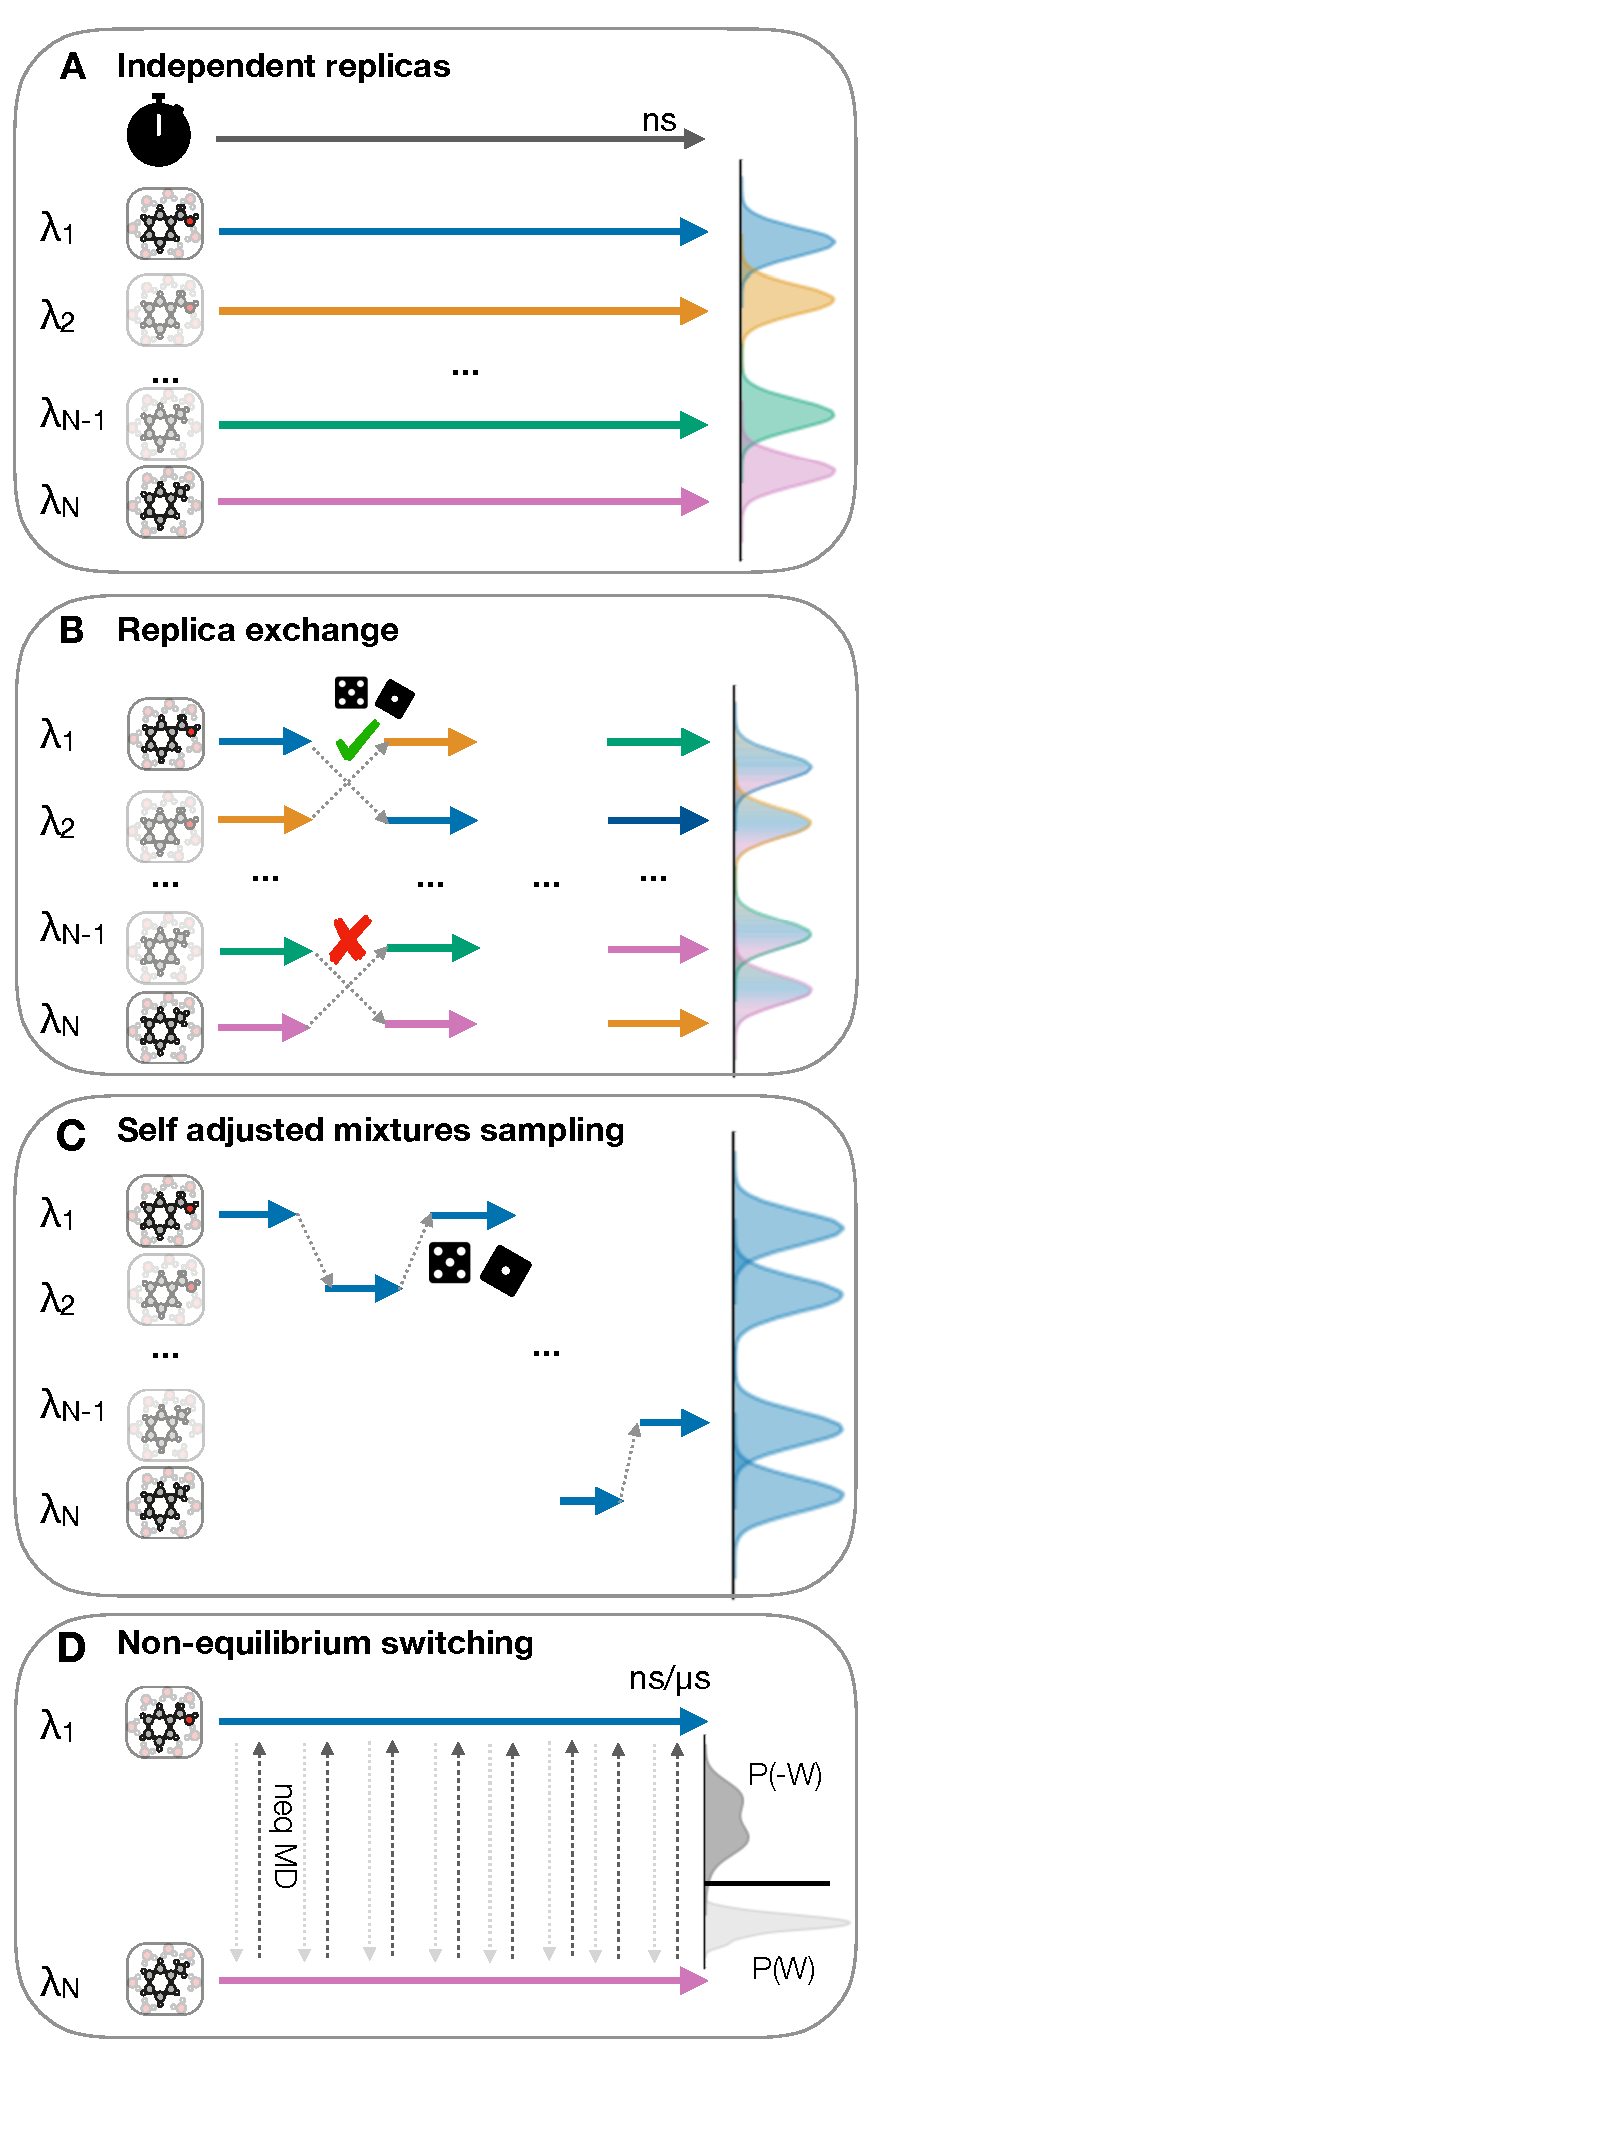
\includegraphics[width=0.95\columnwidth]{figures/fig8_sampl_scheme/Figure.pdf}
    \caption{\textbf{Four most common sampling strategies are available in different popular software packages.} \textbf{A}: Multiple replicas in parallel at different lambda states. \textbf{B}: Hamiltonian replica exchange scheme. \textbf{C}: Single replica scheme sampling from all $\lambda$ states. \textbf{D}: Non-equilibrium sampling scheme.}
    \label{fig:fig_sampling_scheme}
\end{figure} 
The best practice recommendation, is to use replica exchange type sampling schemes (Fig.~\ref{fig:fig_sampling_scheme}(\textbf{B})), or in absence of their availability and when looking at systems with fast mixing times parallel replica schemes are acceptable (Fig.~\ref{fig:fig_sampling_scheme}(\textbf{A})). Single replica schemes and non-equilibrium schemes are not as established yet, but are very promising.

\subsubsection{How long should I run my simulation for and what information should be saved?}
\label{sec:sim_length_information_kept}
Before launching alchemical free energy calculations it is wise to consider how convergence and completion will be assessed. Different conditions on when to stop alchemical free energy calculations should be determined, and this may require several iterative checks and therefore modifications to the calculation protocol.
One useful metric to use for termination is the expected or desired uncertainty of a desired free energy estimate, though care must be exercised should the uncertainty estimate prove unreliable.
In particular, if the rate of change in the free energy estimate is significant when this condition is met, the simulation may not be locally converged, and more sampling may be necessary to determine a stable free energy estimate which is no longer changing significantly over time. 
However, this is not the only metric which should be used, as the uncertainty only captures the information about the sampled phase space, not necessarily the entirety of the phase space.  
For example, convergence of relative free energy calculations in predictive simulations where the entire phase space is not known in advance, requires sampling the different kinetically stable states~\cite{mobley2012perspective}.  
This highlights the importance of choosing the correct thermodynamic path to ensure you sample the required thermodynamic states as discussed in Sec.~\ref{sec:important_path}.
%
The condition of minimizing the statistical uncertainty of different free energy estimators below a sufficient threshold should be one metric monitored over the simulation. This can be done through the uncertainty estimator built into certain analysis tools such as MBAR, or can be done though more general statistical tools like bootstrap sampling. 
A target statistical uncertainty should be chosen at the onset of the simulation to avoid excessively long simulations, or falling into the trap of running until the free energy estimate is "good enough," which is subjective and has no defined criteria. This could be a fixed value such as $0.20 \mathrm{kcal/mol}$, or a functional quantity such as "below $0.5 \mathrm{kcal/mol}$ and $10\%$ of the free energy estimate." The user does not need to monitor this information in real-time and can choose to run simulations for fixed duration (either time or number of samples) and run analysis on the data collected thus far. If more samples are needed, the simulations can be resumed, or, started again in different initial conditions. 
%
Convergence in other alchemical observables should also be monitored to determine if the defined phase space has been sufficiently sampled and enough decorrelated samples have been drawn. These additional observables include, but are not limited to, the variance in $\frac{dU}{d\lambda}$ across all $\lambda$ values, calculating the variance in free energy using bootstrap analysis, and comparing differences in free energies calculated using different percentages of the simulation in both the forward and reverse directions ( see Fig. \ref{fig:convergence_forward_reverse}).
%
\begin{figure}[h!]
    \centering
    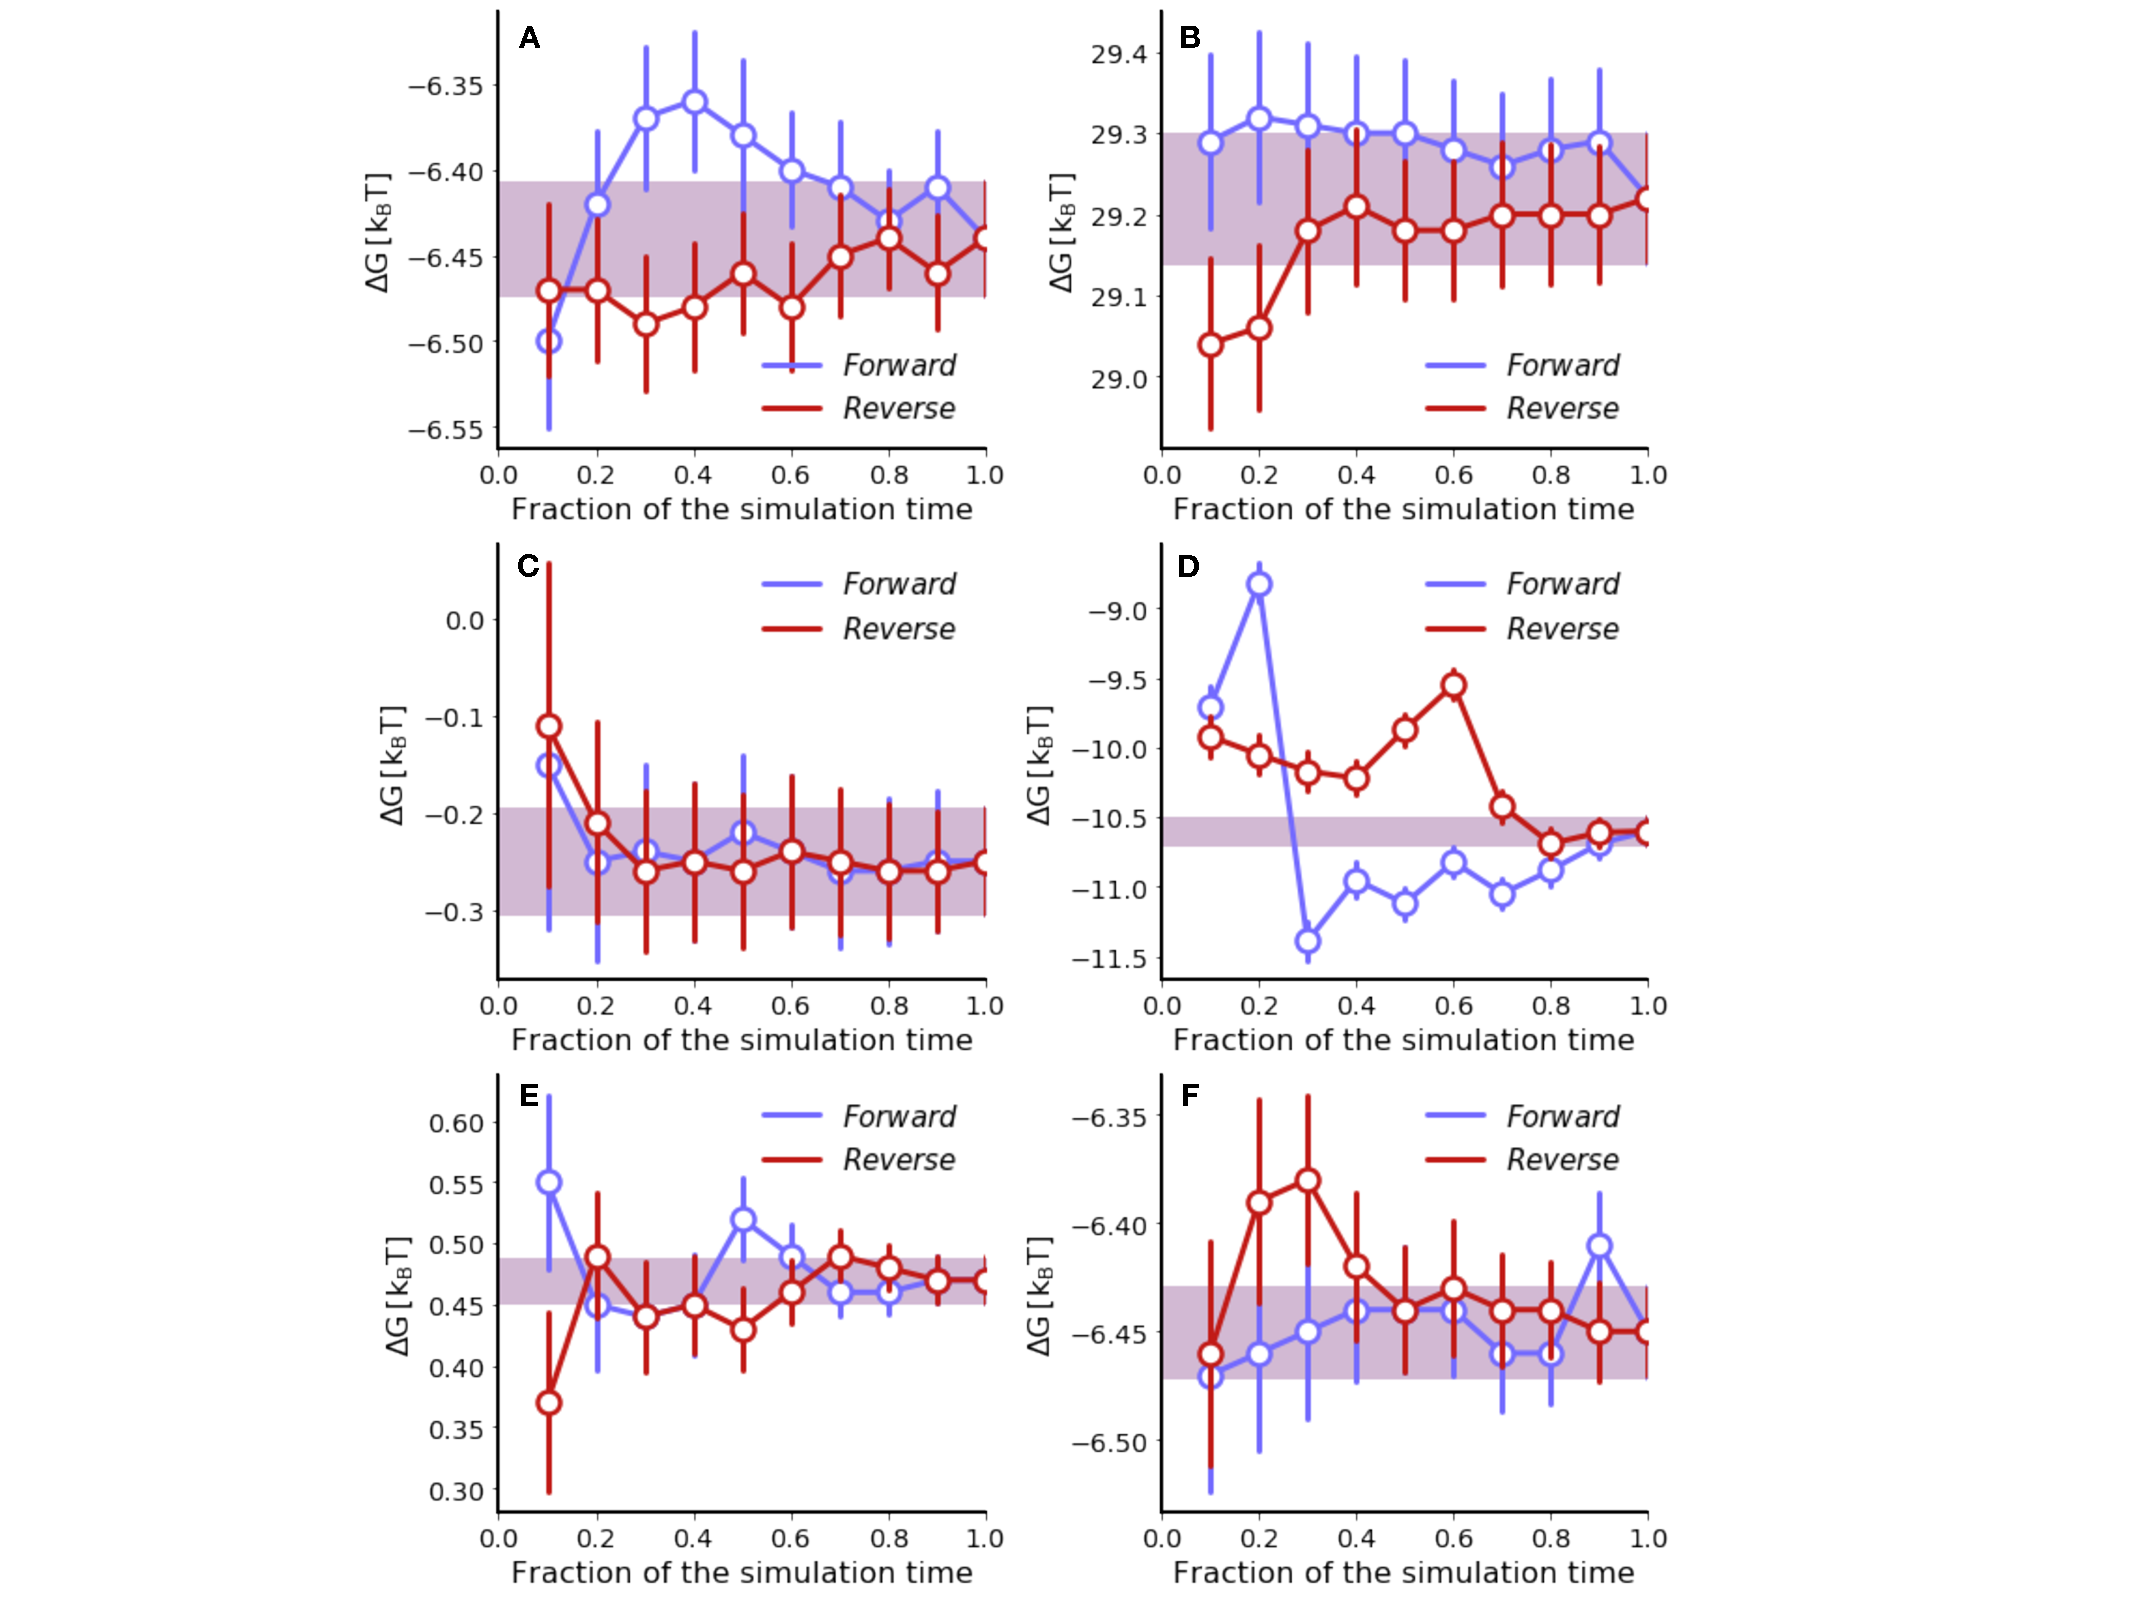
\includegraphics[width=0.95\linewidth]{figures/fig10_forward_reverse/Figure.pdf}
    \caption{\textbf{Free energy (in k$_{B}$T) for two different relative binding free energy (RBFE) perturbations.} 
    Each plot shows the estimated free energy change using a varying fraction of total simulation time (up to 5 ns total). 
    The top panel shows the three-step protocol for a perturbation involving 5 perturbed atoms, while the bottom panel shows the same protocol for a perturbation involving 10 perturbed atoms. The difference in energy between the forward (blue) and reverse (red) free energy calculations at the midpoint of the simulation time gives an indication of the overall convergence of the simulation, with differences over 1 k$_{B}$T indicating poor convergence.}
    \label{fig:convergence_forward_reverse}
\end{figure}
%
Each of these metrics have demonstrated promising results for diagnosing when a simulation has a convergence issue beyond simple convergence of uncertainty estimate. 
Results obtained from calculations with convergence issues should be checked for errors or run for longer before any confidence should be placed in conclusions drawn from their analysis.
In relative calculations that share similar binding modes, for example, and do not induce large conformational changes when in complex with protein, the need to sample exhaustively to converge estimates in free energy differences is often not necessary due to the locality of sampling changes in the molecular topology and shared phase space of the core atoms.
However, even subtly induced changes in protein binding configuration will require more sampling or cause local convergence to a free energy estimate that has high error.
Many enhanced sampling techniques have been proposed to try and overcome barriers in free energy calculations and mitigate convergence to erroneous estimates~\cite{}. 
The confidence a user should have in a free energy estimate is significantly improved when both the uncertainty of the free energy estimate is low, and when other observables have reached a convergence.
%
Another aspect that can be monitored is bias in the simulation. A simple, but effective, way of checking for bias is to compute the same property of interest by multiple estimators (e.g. free energy difference). 
The uncertainty in the free energy, for example, has multiple ways to be estimated, e.g. through standard error propagation methods (including MBAR's estimator, which is based on the same principles as standard error propagation), through bootstrap methods, through multiple independent runs, etc. 
Independent of how the property is estimated, its important to remember that they are \textit{estimations of the property}, not the true underlying property itself. 
These estimators are usually consistent estimators, meaning they will converge to the true answer in the limit of sufficient sampling, not necessarily unbiased ones though.
As such, it is a good idea to subject different estimators to the same data to see if they yield either the same estimate (within error and bias), or if they fluctuate wildly. 
This is not a perfect method as some estimators, such as exponential averaging, will converge significantly more slowly, relative to more accurate estimators like MBAR. 
Therefore, it is a good idea to apply the estimators to different fractions of the data to see if the main estimator of free energy you have chosen is stable.
%
Each method requires different data from the simulation be collected.  If, for instance, the free energy estimator selected is thermodynamic integration, then values of $\frac{dU}{d\lambda}$ at uncorrelated data points must be collected. Once a combination of knowing what type of simulation you will run, which alchemical topology you will simulate, what alchemical path you will simulation along, and what your stopping conditions are, then you are ready to enumerate the information you should capture. Below is a sample of the minimal information you need for a set of common estimators (discussed in more detail in Sec.~\ref{subsec:estimators}):
%
\begin{itemize}
    \item Thermodynamic Integration (TI) requires $\frac{\partial U(\vec{x})}{\partial\lambda}$.
    \item Exponential Averaging (EXP) needs \textit{either} $\Delta U_{k,k+1}(\vec{x})$ or $\Delta U_{k,k-1}(\vec{x})$, depending on the direction its being evaluated in.
    \item Bennett Acceptance Ratio (BAR) needs \textit{both} $\Delta U_{k,k+1}(\vec{x})$ and $\Delta U_{k,k-1}(\vec{x})$.
    \item Weighted Histogram Analysis Method (WHAM) and Multistate Bennett Acceptance Ratio (MBAR) both need the complete set of $\Delta U_{k,j} \, \forall \, j=\{1...K\}$. WHAM must have this information binned.
\end{itemize}
%
The potential derivative required for TI should generally be calculated during the simulation; only under every rare circumstances~\cite{naden2015linear} can it postprocessed by a code that does not evaluate the derivatives. Many codes already have options for doing this.
If that option is unavailable, you can estimate it through finite difference (if sufficient information is collected), but this  will introduce significant error, and is generally not a best practice. The BAR estimator may be a better, and simpler choice at that point as you will have at least the same level of information. 
The potential energy differences required for EXP, BAR, MBAR, and WHAM can be calculated either during the simulation or in post-processing. It is recommended to calculate the potential differences in code when possible to avoid extra overhead and possible errors produced by running the simulation twice, and to reduce the amount of stored information. 
Although TI must be usually be calculated in code, as it requires the derivative, there is one condition under which it actually has the fastest computation time. 
If the alchemical path you have chosen is a linear alchemical path, then you get $\frac{dU}{d\lambda} = U_0(\vec{x}) - U_1(\vec{x})$, which is the difference between the initial and final states. 
However, because of the problems with linear paths already discussed in this paper, this simplification is rarely that useful.
%
Free energy information should generally be saved more frequently than coordinate data, approximately at the rate that uncorrelated samples are produced.  
The on-disk size of the data for free energy estimation is often significantly smaller than full atomic coordinates, so the information should be collected frequently. 
However, the information should not be collected \textit{every} time step, as most free energy techniques are operated at equilibrium, and need equilibrated \textit{and decorrelated} samples for an unbiased estimate.
A sample collected every time step will likely result in most samples being discarded due to decorrelation routines in the analysis. However, if it is computationally cheap and disk space is plentiful, do save often. One may safely assume that the correlation time is greater than 100-200 fs even for relatively simple systems such as small molecules in solvent, so saving no more frequently than every 50-100 steps is recommended. 
How decorrelation impacts calculations, and how to compute it is discussed in other section~\ref{sec:decorrelating-samples}. 
%
\subsubsection{Multiple or uncertain binding modes may require considerable care}
\label{sec:multiple_binding_modes}
In a discovery setting, new ligands typically have unknown or at least uncertain binding modes~\cite{kaus2015how, plountprice2000analysis,mobley2009binding,calabro2016elucidation},  complicating binding free energy estimation.
This uncertainty is because it is usually not desirable to estimate a binding affinity for a ligand which already has an available bound structure, since such a compound has already been tested.
To deal with prospective ligands with unknown binding modes, discovery projects commonly assume that modifications of functional groups on a common scaffold result in a consistent binding mode across all members of a series.
This is not necessarily always the case~\cite{kaus2015how}, as reviewed elsewhere~cite{mobley2009binding} and in some cases unexpected binding mode changes can be the origin of apparent non-additivity in structure-activity relationships~\cite{calabro2016elucidation}.
Binding modes also tend to be particularly variable in the case of fragments, which often may have multiple relevant binding modes~\cite{}.
%
Absolute free energy calculations for dissimilar ligands can have particular challenges because the (potentially incorrect) assumption of consistent binding modes across a series of similar ligands is likely to be even less robust than the in the case of relatively calculations.
This means that researchers performing absolute binding free energy calculations will have to pay particular attention to generating reasonable putative binding modes.
%
In some cases, it is tempting to simply use docking techniques to generate initial bound structures for starting molecular dynamics simulations.
However, timescales for binding mode interconversion are usually slow compared to MD/free energy timescales, meaning that simulations started from different potential binding modes are likely to yield disparate computed binding free energies~\cite{mobley2006use, palma2012computation, mobley2012perspective, gill2018binding} .
And docking techniques are good at identifying sterically reasonable potential binding modes, but still perform relatively poorly at identifying a single dominant binding mode \emph{a priori}.~\cite{} 
%
It is worth highlighting a recent SAMPL blind challenge on HIV integrase as an illustration of this. 
Many submissions, using state-of-the-art methods, had difficulty even predicting which \emph{binding site} ligands would bind in (most submissions placed more than half of the ligands into the incorrect binding site), and even given correct binding sites, the binding mode within each site was also quite difficult to predict~\cite{mobley2014blind}.
The best performing submission for predicting binding modes actually ended up being a human expert (aided by computational tools) with more than 10 years of experience on the particular target~\cite{voet2014combining}, rather than a fully automated approach.
While free energy calculations on this set had some success, many of the failures actually ended up being cases where the binding mode selected as input for free energy calculations was later found to be incorrect~\cite{gallicchio2014virtual}, highlighting the importance of these issues.
%
One approach which has shown some success is to retain diverse potential binding modes from docking, perform short MD simulations of these to identify distinct stable binding modes, and then consider these in subsequent calculations~\cite{gallicchio2014virtual, mobley2006use,rocklin2013blind, boyce2009predicting, mobley2007predicting}.
%
Routes to handle multiple potential binding modes are different depending on whether absolute or relative calculations are selected, unless a method is available to estimate the relative populations of different stable binding modes in advance (e.g. such as the BLUES approach currently in development~\cite{gill2018binding}), in which case this approach could be applied to assist both types of calculations.
%
\paragraph{Handling multiple potential binding modes within absolute calculations.}
Within absolute binding free energy calculations, multiple potential binding modes can be handled by two main strategies: Consider each binding mode separately (a separation of states strategy) or sample all binding modes within a single simulation~\cite{mobley2012perspective}.
This couples to the choice of restraints selected, as some restraints will allow transitions between binding modes and even binding sites (Section~\ref{sec:standardstate-restraints}), and others do not.
%
Sampling all binding modes within a single free energy calculation is usually impractical without some form of enhanced sampling or at least Hamiltonian replica exchange~\cite{wang2013identifying} because barriers for binding mode interconversion result in kinetics which are too slow compared to simulation timescales~\cite{mobley2006use, palma2012computation,mobley2012perspective, gill2018binding}.
Hamiltonian exchange, coupled with appropriate restraints, can allow the ligand to relatively rapidly exchange between potential binding modes when non-interacting, accelerating sampling of binding modes~\cite{wang2013identifying}.
\todo[inline, color={yellow!40}]{DLM probably need more background refs on Hamiltonian lambda exchange here.}
%
Separation of states provides a simple though potentially expensive alternative, where each stable binding mode is considered separately with a binding free energy calculation restricted to that binding mode, and then (as long as the binding modes are non-overlapping) the resulting component binding free energies can be combined into a total~\cite{mobley2006use, mobley2012perspective}.
This approach necessitates a separate binding free energy calculation for each potential binding mode, however, so it can be computationally quite costly.
If relative populations of different stable binding modes were available from some other technique, it could make this separation of states approach considerably more efficient~\cite{mobley2012perspective, gill2018binding}.
%
\paragraph{Handling multiple potential binding modes within relative calculations.}
Multiple potential binding modes pose particular problems for relative free energy calculations, as having multiple starting structures for these calculations could yield substantially different calculated relative binding free energies for the same transformation due to kinetic trapping, and, without additional information (specifically, the free energy of binding mode interconversion or, equivalently, the relative populations of different binding modes) it becomes impossible to sort out which of the multiple answers is in fact the correct relative binding free energy~\cite{}.
%
To deal with this, some practitioners have actually computed relative binding free energies of different binding modes of the same ligand~\cite{palma2012computation}.
For example, a perturbation which adds a methyl to an aromatic ring of a larger ligand might yield one result if the methyl points in one direction, and a different value if it points in the other due to slow ring motions. [e.g. get ref from Sukanya]
One could compute the free energy of turning off the methyl group in one orientation and turning it back on in the other orientation to obtain the free energy difference between the two potential binding modes.
While this approach has precedent, it is relatively difficult to automate at present and requires considerable care.
%
Overall, this likely means that relative free energy calculations will be susceptible to problems resulting from uncertainty in ligand binding modes until more robust approaches are available to determine dominant binding modes, or the relative populations of different potential binding modes, in advance.
%
%%%%%%%%%%%%%%%%%%%%%%%%%%%%%%%%
%  Data Analysis               %
%%%%%%%%%%%%%%%%%%%%%%%%%%%%%%%%
\section{Data analysis}
\label{sec:data_analysis}
Once data has been collected from alchemical intermediates, it must be analyzed to produce an estimate of the free energy change (and its associated statistical uncertainty) for each leg of the thermodynamic cycle.
While a number of different estimators are available that will give consistent results under optimal circumstances, some approaches are recommended over others due to their robustness and ability to provide information on poor convergence.
%
\subsection{Detecting the boundary between equilibrated and production regions}
\label{sec:automatic-equilibration-detection}
Much of the infrastructure for analyzing alchemical free energy calculations relies on the concept of asymptotically unbiased estimators, which produce unbiased estimates of the free energy when fed very long simulations~\cite{shirts2005comparison}.
In reality, free energy calculations are often initiated from highly atypical initial conditions (such as a protein-ligand geometry obtained from docking and subjected to a heuristic solvent placement scheme), and simulations are of a finite length dictated by available computational resources and computing demands.
As a result, these estimators can produce significantly biased estimates if fed the entirety of simulation data generated without further processing~\cite{chodera2016simple}.
%
\begin{figure}
    \centering
    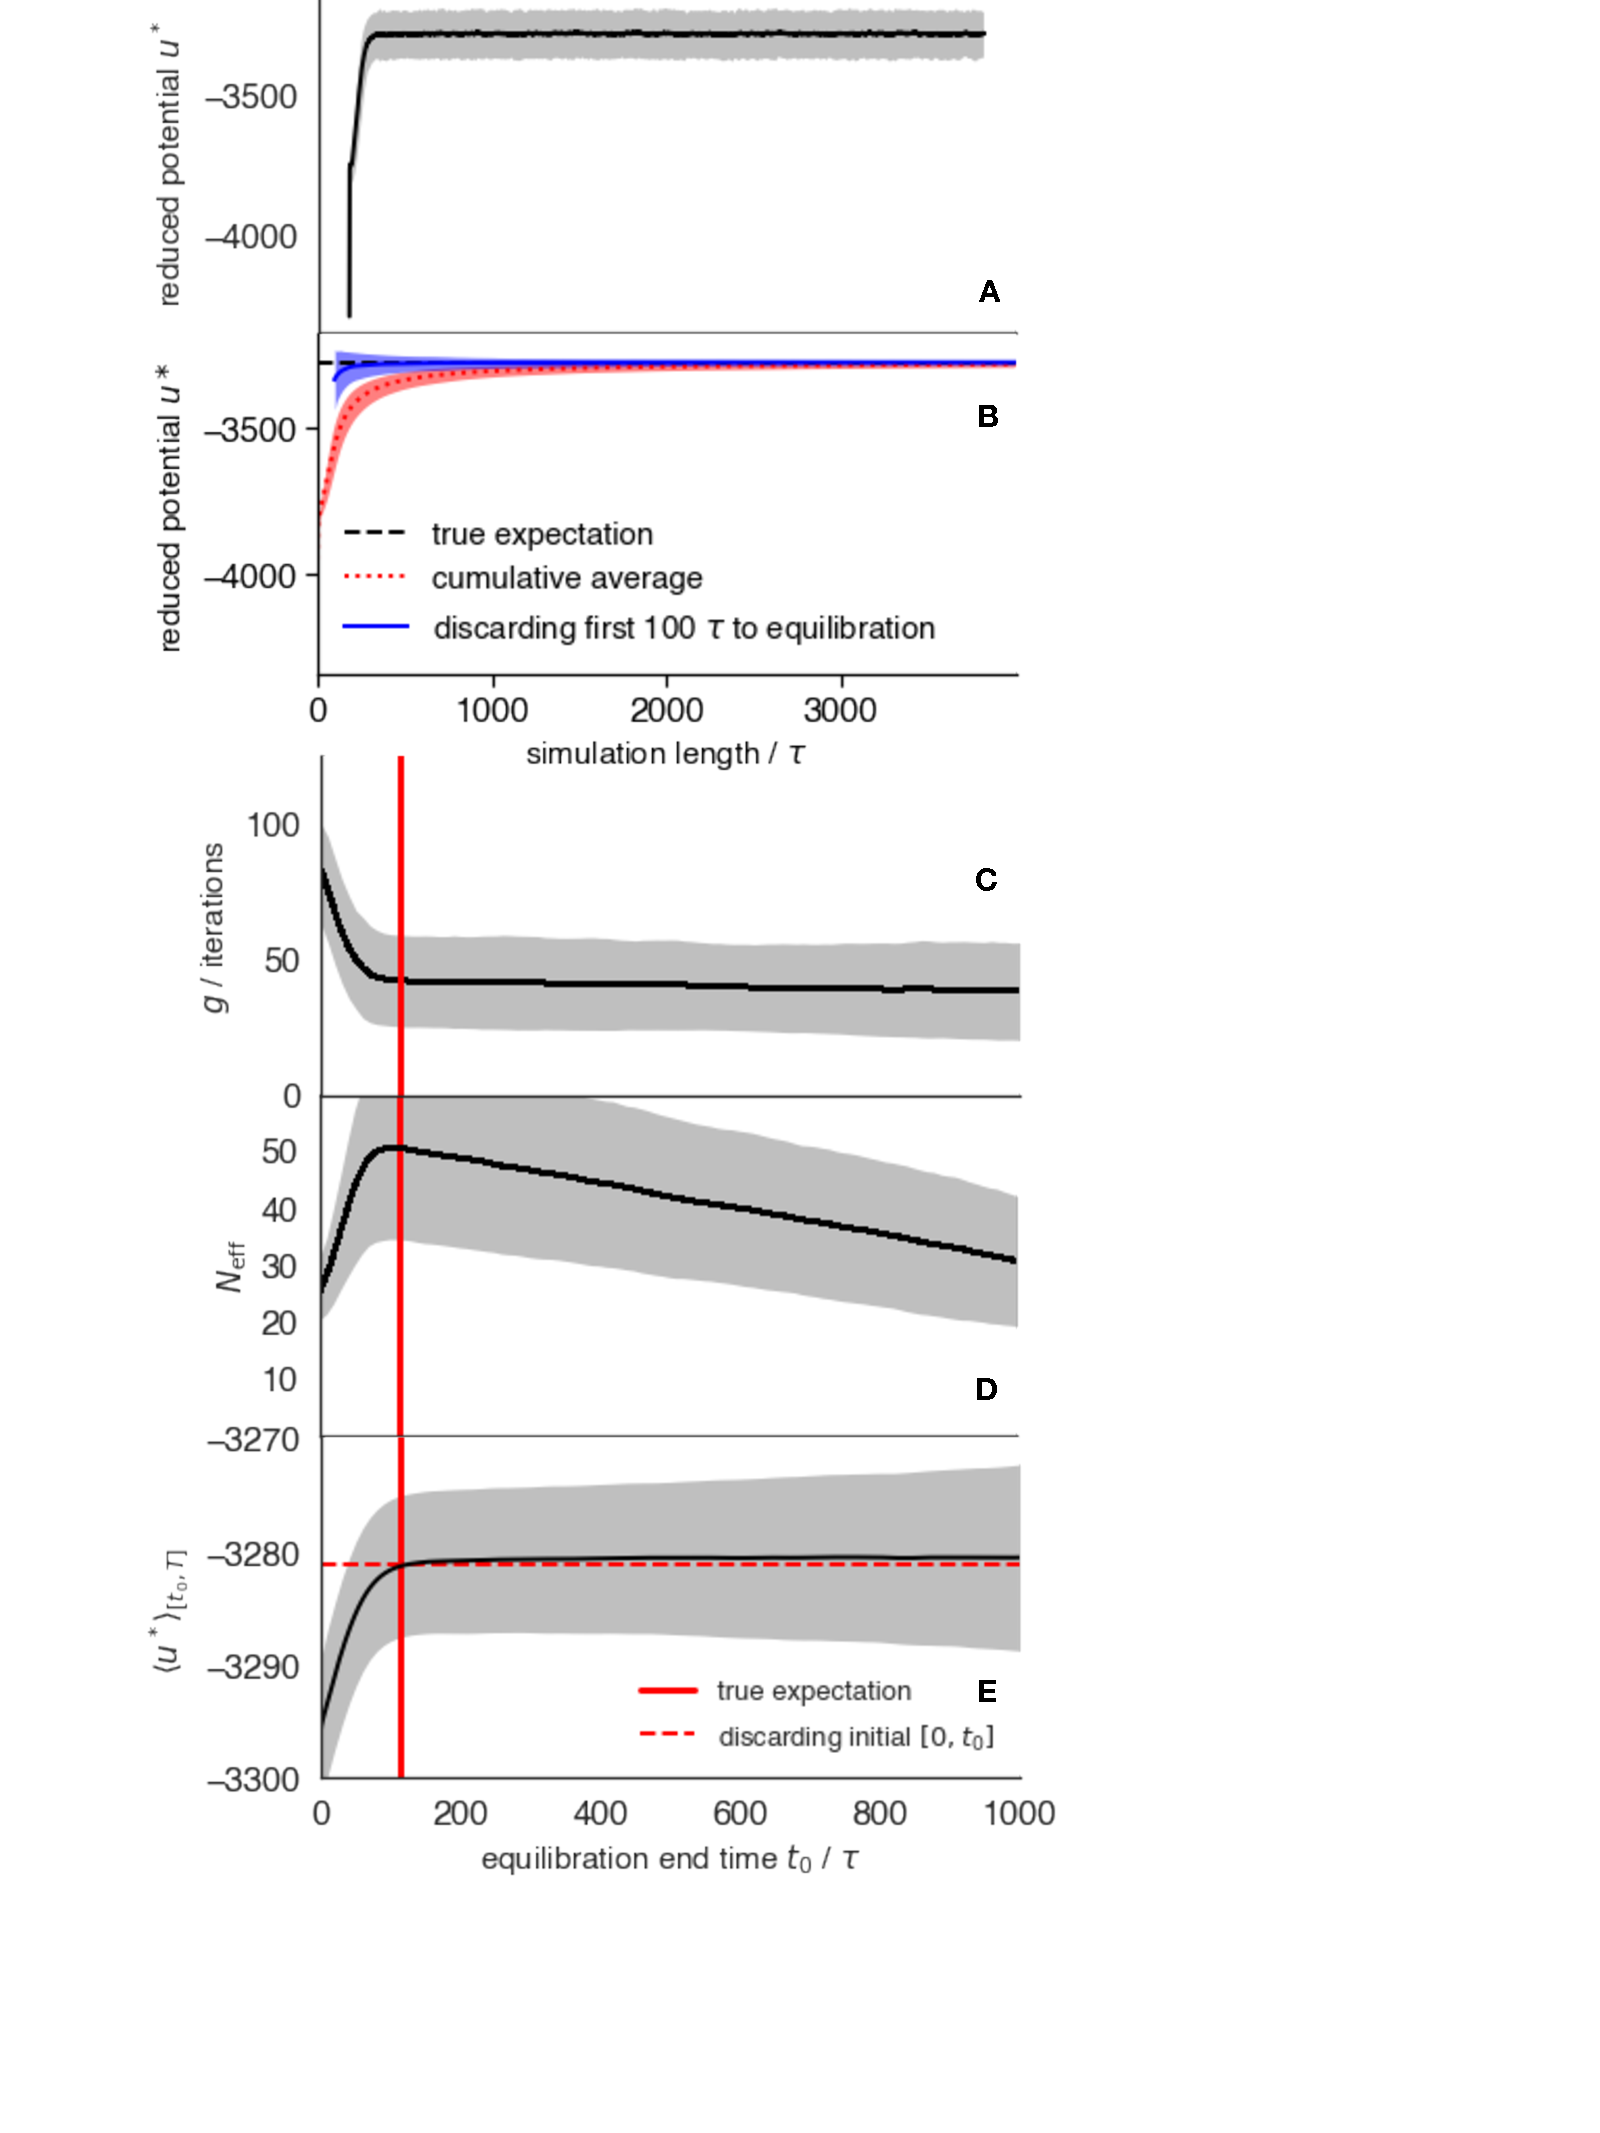
\includegraphics[width=0.95\linewidth]{figures/fig11_equib_detection/Figure.pdf}
    \caption{{\bf Automatic partitioning into equilibration and production regions.}
    \textbf{A} The average (black line) standard deviation (shaded region) of the reduced potential $u^*$ over many independent replicate simulations started from the same initial conditions show a significant initial transient change before relaxing to the true average potential energy \textbf{B}. A cumulative average (red) of the entire simulation data demonstrates simulation bias not seen when initial simulation data is omitted (blue). Using an automated approach to detect equilibration of the boundary $t_0$ using statistical inefficiency $g$ (\textbf{C})  for an effective simulation interval (\textbf{D}). \textbf{E} The optimal equilibration boundary $t_0$ is selected to maximize the number of uncorrelated samples.
    \emph{Figure adapted from~\cite{chodera2016simple}.}
    }
    \label{fig:automatic-equilibration-detection}
\end{figure}
%
To minimize this effect, an initial portion of the simulation is often discarded to \emph{equilibration}~\cite{braun2019best}, with the idea of removing the most heavily biased initial portion of simulation data but retaining the unbiased \emph{production} region that represents a stationary Markov chain process sampling from the desired equilibrium target distribution.
Because the simulation time required for the atypical initial sampler state to relax toward equilibrium is a property of the specific system being simulated and the specific initial conditions selected, it is simplest to collect data for the whole process and use an automated algorithm to select how much data should be discarded to equilibration in a post-processing step.

A simple approach to automatically partitioning simulation data into equilibration and production regions is described in~\cite{chodera2016simple} (illustrated in Figure~\ref{fig:automatic-equilibration-detection}).
Suppose we have a simulation of length $T$ consisting of correlated data.
Here, the goal of the post-processing step is to select the equilibration boundary $t_0 \in [0, T]$ so as to \emph{maximize} the number of effectively uncorrelated samples remaining in the production region $N_{[t_0,T]}$, which is defined as
\begin{eqnarray}
N_{[t_0,T]} &=& \frac{T - t_0}{g_{[t_0,T]}}
\end{eqnarray}
where $g_{[t_0,T]}$ is the \emph{statistical inefficiency} of a timeseries $a_t$, described in more detail below.
Conveniently, this procedure also produces the information necessary to decorrelate the simulation data for estimating the free energy differences, a requisite next step in analysis.
This approach is implemented within the MBAR~\cite{kylebeauchamp2019choderalab} and alchemlyb~\cite{daviddotson2019alchemistry} packages, and is highly recommended for standard practice.
%
For additional discussion of working with correlated data and autocorrelation analysis, please refer to the work on Best Practices for Quantification of Uncertainty and Sampling Quality in Molecular Simulations~\cite{grossfield2018best}.
%
\paragraph{Computing the timeseries for equilibration detection}
Typically, the timeseries of note $a_t$ analyzed in automated equilibration detection is the negative logarithm of the probability density sampled by the MCMC algorithm (up to an irrelevant additive constant).
For simple independent simulations that sample $x_t \sim \pi(x ; \lambda)$, this is given by the reduced potential
\begin{eqnarray}
a_t &\equiv& - \ln \pi(x_t; \lambda) + c = u(x_t; \lambda) .
\end{eqnarray}
%
Note that the use of the effective reduced potential is not guaranteed to pick up on all slow relaxation processes that may be coupled to the alchemical free energy, but the simplicity of its computation means it is generally appropriate for most cases.
%
\paragraph{Cautions in automating equilibration detection}
For simulations that are simply not long enough to contain a large number of samples from true equilibrium either because they are very short or contain slow processes, this procedure cannot completely remove the bias.
In such cases, this approach simply selects the final portion of the the simulation, which may be contained in a single substate of conformational space, which may itself lead to biased estimates. 
This situation can be detected if the equilibration boundary $t_0$ is a significant fraction of the total simulation length $T$, with a good rule of thumb being that $T \gtrsim 20 t_0$.
If this is not possible, advanced analysis techniques that assume only local equilibrium (rather than global equilibrium) such as the TRAM estimators~\cite{mey2014xtram,wu2016multiensemble,nuske2017markov} may be more appropriate, but are beyond the scope of this paper. 
%
\subsection{Decorrelating samples for analysis}
\label{sec:decorrelating-samples}
\paragraph{Computing the statistical inefficiency}
Most estimators require an uncorrelated set of samples from the equilibrium distribution to produce (relatively) unbiased estimates of the free energy difference and its statistical uncertainty.
To do this, the production region of the simulation is generally \emph{subsampled} with an interval approximately equal to or greater than the \emph{statistical inefficiency} $g \ge 1$ to produce a set of uncorrelated samples that can be fed to the estimator machinery~\cite{chodera2016simple},
\begin{eqnarray}
g &\equiv& 1 + 2 \tau_\mathrm{eq} \label{eq:statistical-inefficiency-definition}
\end{eqnarray}
where $\tau_\mathrm{eq}$ is the integrated autocorrelation time, formally defined as
\begin{eqnarray}
\tau_\mathrm{eq} &\equiv& \sum_{t=1}^{T-1} \left(1 - \frac{t}{T}\right) C_t \label{eq:integrated-autocorrelation-time-definition} , 
\end{eqnarray}
with the discrete-time normalized fluctuation autocorrelation function $C_t$ defined as
\begin{eqnarray}
C_t &\equiv& \frac{\expect{a_n a_{n+t}} - \expect{a_n}^2}{\expect{a_n^2} - \expect{a_n}^2} . \label{equation:autocorrelation-definition}
\end{eqnarray}
The basic concept is that $\tau_\mathrm{eq}$ corresponds to the single-exponential decay time for the autocorrelation process that generates samples, so the statistical inefficiency $g$ measures the approximate temporal separation between two effectively uncorrelated samples (where two exponential relaxation times are presumed to be sufficient).
%
Robust estimation of $C_t$ for $t \sim T$ is difficult due to growth in statistical error, so common estimators of $g$ make use of several additional properties of $C_t$ to provide useful estimates (see \emph{Practical Computation of Statistical Inefficiencies} in~\cite{chodera2016simple} for a detailed discussion).
\todo[inline]{JDC: Describe recommended statistical inefficiency computation algorithm.}
We recommend using the robust statistical inefficinecy computation routines available within the MBAR~\cite{kylebeauchamp2019choderalab} and alchemlyb~\cite{daviddotson2019alchemistry} packages.
%
\paragraph{Subsampling data to generate uncorrelated samples}
Once the statistical inefficiency $g$ has been estimated, it is straightforward to subsample the correlated timeseries simulation data to produce effectively uncorrelated data that can be fed to estimators of the free energy.
Suppose the correlated timeseries is $\{a_t\}_{t=1}^T$; we can form a new timeseries of $N_{\mathrm{eff}} \approx T / g$ effectively uncorrelated samples by selecting a subset of indices $\{ \: t = \mathrm{round}((n-1) \, g) \: | \: n \in \mathrm{range}(1,\ldots ,N) \: \}$ where $\mathrm{round(x)}$ denotes rounding to the nearest integer.
%
If independent simulations are used, the alchemical state $\lambda$ may have a significant impact on the correlation time, and these simulations should be subsampled independently using a separate estimate of the statistical inefficinecy $g$ for each alchemical state.
If coupled simulations are used (such as a Hamiltonian replica exchange simulation), the replicas should undergo equivalent random walks in alchemical space, and the replicas can be can be subsampled with the same $g$ to generate an equal number of uncorrelated samples at each alchemical state.
Conveniently, the approach described above for automated equilibration detection produces an appropriate estimate of $g$ over the production region for automating this process.
%
\paragraph{Cautions and considerations}
Reliable estimation of the statistical inefficiency is difficult, and estimates will not generally be as precise (in a relative error sense) as averages.
To ensure there is sufficient data available for reliable decorrelation and estimation of free energy differences, it is recommended that the effective number of uncorrelated samples $N_{\mathrm{eff}} \ge \approx 50$ if the BAR or MBAR estimators (discussed below in sec~\ref{subsec:estimators}) are used; the number may need to be much higher with alternate estimators.
%
\subsection{Estimators for free energy differences}
\label{subsec:estimators}
Free energy differences between two different states differing in the energy function are directly related to the
ratio of probabilities of those states.
As can be noted, the partition functions in Eq.~\ref{equation:dimensionless-free-energy-difference} are simply the total accumulated probabilites for all possible configurations of the system. Virtually all of the ways to estimate this free energy are based in converting this ratio of integrals to something that can be measured in one (or several) simulations.  
%
\paragraph{The Zwanzig relationship (EXP)}
%
The simplest method for calculating free energy differences from simulations is the so-called \textit{Zwanzig
relationship}~\cite{zwanzig1954hightemperature}, also called one-sided exponential reweighting (EXP), or simply free energy perturbation, thought this final term is sometimes used to encompass all ways of calculating free energy differences.
%
The (reduced) free energy difference $\Delta f_{01}$ between an initial state 0 and a final state 1 defined by two different potential energy functions 
$U_0(\vec{q})$ and $U_1(\vec{q})$ over coordinate space $\vec{q}$ can be calculated as:
\begin{eqnarray}
\Delta f_{01} & = & \ln \expect{e^{-(U_1(\vec{q}) - u_0(\vec{q}))}}_0 =  \ln \expect{e^{-\Delta u(\vec{q})} }_0
\end{eqnarray}\label{eqn.zwanzig}
and the average is over all samples from the simulation performed with $u_0$. In the case of NVT (canonical) sampling and assuming the masses do not change, then $u$ is just $U/k_BT$, and $f$ is $F/k_BT$, but it can be generalized to other ensembles with the proper definition of $f$ and $u$.
Described in words, we take the samples generated during our run with the potential energy function $U_0(\vec{q})$, recalculate what the energy difference would be if we switched to potential energy function $U_1(\vec{q})$, and average the exponential of the -1 times the energy difference to get -1 times the exponential of the free energy difference. The original distributions (P($U_0$) as generated at $\lambda=0$ and P($U_1$) would look like the ones seen in figure~\ref{fig:fig_sampling_scheme} (A)-(C)on the left hand side. Reevaluating  requires almost no extra code functionality to perform; one need only to save a full precision trajectory, and run an unmodified molecular simulation code using the $U_1$ in order to calculate the new energies of stored snapshots. The analysis can be written in a line of code.  We note that this method is even more general, in that the instantaneous work to change the potential energy function from $U_0$ to $U_1$ can be replaced by the non-reversible work $W$ to make the same change under the same equilibrium conditions at either end state~\cite{jarzynski1997nonequilibrium,jarzynski1998equilibrium,crooks2000pathensemble}, though we do not go into all of the details of non-equilibrium transformations here, and refer the reader to more advanced treatments~\cite{maragakis2008bayesian,oberhofer2005biased,procacci2015unbiased,shirts2003equilibriuma,ytreberg2004singleensemble}
%
Although the Zwanzig equation is formally correct (as long as the two states considered sample the same phase space volume, which is true for standard molecular models), it has some very important numerical issues that mean that it often performs badly for standard free energy calculations, even for small molecules~\cite{shirts2005comparison,lu2003appropriate}.  One can show that if the standard deviation of the difference $\Delta U(\vec{q}) = U_1(vec{q})-U_2(\vec{q})$ over all sampled $\vec{q}$ is large (which in this case, means only several times $k_BT)$, then very few samples contribute to the average, and the answer will be both biased and extremely noisy~\cite{lelievre2010free}. Essentially, the method is dominated by contributions of rare snapshots\cite{jarzynski2006rare, wu2005phasespaceb, wu2005phasespacec}. There are a number of applications where it this expression is nevertheless useful, but those usually involve investigating the dependence of the free energy on small changes in parameters, not changing molecules or even single atoms in molecules~\cite{xx}
%
\paragraph{The Bennett Acceptance Ratio (BAR)}
%
If we have the differences in the potential energy sampled from the distribution defined by $U_0$ to the state defined by $U_1$, and we also have the differences in potential energies from the distribution sampled by $U_1$ to the state defined by $U_0$, we can obtain a significantly improved estimate of the
free energy difference compared to that obtained by EXP. 
This estimate was first derived by Bennett and is hence generally called the Bennett Acceptance Ratio (BAR).  It is solved by finding the reduced free energy $f_{ij}$ that satisfied the following implicit equation:
\begin{eqnarray}
 \sum_{i=1}^{n_i} \frac{1}{1 + \exp[\ln(\frac{n_i}{n_j}) + u_{ij}(\vec{q}) - f_{ij})
 ]} \nonumber \\
 =\sum_{i=1}^{n_j} \frac{1}{1 + \exp[\ln(\frac{n_i}{n_j}) - U_{ij}(\vec{q}) + f_ij)]},
\end{eqnarray}
where $n_i$ and $n_j$ are the number of samples from each state. We
will refer to this method as BAR. More recent derivations show that this formula is the maximum likelihood estimate of the free energy difference given sets of samples from the two states~\cite{bennett1976efficient,shirts2003equilibriuma }. 
%
Many studies have demonstrated both the theoretical and practical superiority of BAR over EXP in molecular
simulations~\cite{shirts2005comparison,lu2003appropriate}, and BAR converges to EXP in the limit that all samples are from a single state~\cite{bennett1976efficient,bennett1976efficient,shirts2003equilibriuma}. BAR also requires significantly less overlap between the configurational space of each state to converge than EXP, though some overlap must still exist.
%
The Bennett acceptance ratio is only defined between two states. Usually, the endpoints of interest in a free energy calculation are sufficiently different that we will need a chain of states that gradually change the potential energy function from $U_0$to $U_1$, as discussed in Section~\ref{sec:important_path}. You can simply carry out BAR between each pair of states $\Delta G_{1 \rightarrow N} = \Delta {G_{1\rightarrow 2}} + \Delta {G_{2\rightarrow 3}} +  \ldots + \Delta G_{N-1\rightarrow N}$.
%
There is one important thing to note about the uncertainty estimates when summing multiple free energies together to calculate an overall free energy estimate. Although BAR itself gives a free energy estimate that is asymptotically correct in and is much less biased than the uncertainty estimate for EXP, the uncertainties in $\Delta {G_{i-1\rightarrow i}}$ and $\Delta {G_{i\rightarrow i+1}}$ are not uncorrelated, because they both involve the energies $U_i(\vec{q})$. The variances of each of the free energies will \textit{not} propagate as variances usually do (in quadrature) to the variance of the overall free energy. Instead, some other method for propagating the uncertainty, such as bootstrapping~\cite{grossfield2018best} must be used.
%
\paragraph{Thermodynamic integration (TI)}
By taking the derivative of the free energy with respect to the
variable $\lambda$, we find that:
\begin{equation}
\frac{df}{d\lambda} = \frac{d}{d\lambda} \ln \int \exp{-u(\lambda,\vec{q})} d\vec{q} = \expect{\frac{du(\lambda,\vec{q})}{d\lambda}\
}_{\lambda} 
\end{equation}
And than we can then numerically integrate $df/d\lambda$ over an alchemical transformation, using a range of different well-established techniques, to obtain:
\begin{equation}
\Delta f    = \int_{0}^{1} \expect{\frac{du(\lambda,\vec{q})}{d\lambda}}_{\lambda}  d\lambda    
\end{equation}
This approach to calculating the free energy is called thermodynamic integration (TI). Averaging over $\expect{\frac{du}{d\lambda}}$ requires fewer uncorrelated samples to reach a given level of relative error
than averaging $e^{-u(\vec{q})}$, as the range is usually narrower with a more Gaussian distribution. Rather than being limited by overlap, as in the case of BAR and MBAR (see below), we are instead limited by the bias in the numerical quadrature, which must be minimized sufficiently to be beneath the level of statistical noise.
%
Various numerical integration schemes are possible, but the trapezoid
rule provides a simple and robust scheme.  All types of numerical integration can be written as:
\[ \Delta f \approx \sum_{k=1}^{K} w_k
\expect{\frac{du(\lambda,\vec{q})}{d\lambda}}_{k} \] where the weights $w_k$ correspond to a particular choice of numerical integration.
Researchers have tried a large number of different integration schemes~\cite{resat1993studies,jorge2010effect,shyu2009reducing}. However, many other integration choices require specific choices of $\lambda$ to minimize bias, which makes them unsuitable when the intermediates
have widely-varying levels of uncertainty. For example, integrating a cubic spline interpolation provided negligible benefits~\cite{paliwal2011benchmark}. For starting researchers, we therefore recommend a simple trapezoid rule scheme, as it allows for maximal flexibility in which values of $\lambda$ are simulated.  Because fitting to higher order polynomials can have numerical instabilities for some energy functions, and because alternate functional forms might only be appropriate with some types of transformations, expertise and experience is required to perform such numerical integration modifications. In practice, adding 2-3 more intermediate states is typically sufficient to match the performance of these more complicated numerical quadrature schemes.
%
One drawback of TI is that it requires derivatives with respect to $\lambda$ to be calculated directly in the code. Unfortunately, many problems of interest require using pathways (such as the soft-core pathways, for removing repulsive interactions) that are not linear, as we discuss, making this more complex. Still, if the code of interest does compute $\frac{du}{d\lambda}$, then TI is perhaps the simplest method to use, as it involves a very little post-processing.
%
\paragraph{The multistate Bennett acceptance ratio (MBAR)}
One can generalize Bennett's logic from two states to multiple states to obtain a free energy estimator that uses energy differences between all intermediate states. MBAR gives a system of implicit equations for the free energies $f_i$:
\begin{equation}
f_i = - \ln \sum_{n=1}^{N} \frac{\exp(-u_i(\vec{q}_n))}{\sum_{k=1}^K N_k \exp(f_k-u_k(\vec{q}_n))}
\end{equation}
where there are $N_k$ samples from each of $K$ states, with $\sum_k N_k=N$ the total number of samples. Thus, we need to evaluate the energy function $U_i$ for all samples obtained at all states in the transformation. The equations can be solved by a number of different standard routines. We note that there are only $K-1$ independent equations, so only K-1 of the free energies are independent variables, and one of the $f_i$ must be specified (usually, without loss of generality, setting it to zero).
%
MBAR is provably the lowest variance asymptotically unbiased estimator of the free energies given the energies of the samples~\cite{tan2004likelihood}, which means that BAR is also for the free energy difference between only 2 states, as it is mathematically exactly the same as MBAR in this case. MBAR also provides an uncertainty estimate, derived from standard error propagation methods, which has been shown to be accurate as long as there are sufficient samples at each state~\cite{paliwal2011benchmark}.
%
MBAR can also be thought of as the Zwanzig estimator of the free energy to state $i$ where the sampled distribution is the \textit{mixture distribution} of all the other samples thrown together in one ``pot'', defined by $p_m(\vec{q}) = N^{-1} \sum_k  N_k \exp(f_k-u_k\vec{q})$, the weighted average of all the individual normalized probability distributions that are performed.~\cite{shirts2017reweighting}.
%
\paragraph{Recommendations}
\begin{itemize}
\item We recommend MBAR if all energy differences are available. It is provably the lowest variance free energy estimate given samples from multiple states.
\item BAR is essentially just as good as MBAR for highly optimized $\lambda$ intermediates. Specifically, if the $\lambda$s are chosen such that intermediate states have moderate overlap with their neighbors (i.e. between $i$ and $i+1$ and between $i$ and $i-1$, they will \textit{not} have significant overlap with their next nearest neighbors $i+2$ and $i-2$. Thus MBAR does not actually get significant information from these energy differences, so one might as well not even calculate them, and just perform BAR between nearest neighbors.~\cite{paliwal2011benchmark} 
\item TI usually gives similar values as MBAR implemented with sufficient numbers of intermediates, but quadrature errors are hard to estimate beforehand.~\cite{paliwal2011benchmark}
\item WHAM is an approximation to MBAR, and there are no compelling reasons it should be used. 
\item Other variants, especially ones that adaptively determine the free energies can be  useful in certain circumstances but beyond the scope of a Best Practices article.
\end{itemize}
%
\subsection{Uncertainty estimation}
\label{subsec:uncertainty}
It is important to consider the variation in your computed free energies from your equilibrium simulations and in this way obtaining an estimate on the certainty, or uncertainty of the obtained value for the free energies you are interested in. A recent best practices paper by Grossfiled et. al~\cite{grossfield2018best} goes into great detail on estimating uncertainties from molecular simulations and is a good starting point for this topic. 
In general the quantification of different error metrics depends on both data generation and analysis methods  used from the ones discussed above. 
%
The computation of free energies using TI (section~\ref{subsec:estimators}) is straightforward and the trapezoidal rule is often recommended since it allows unequal spacing of $\lambda$ states, which is required to minimize the variance in the free energy estimate, but in principle any good numerical integration method can be used. 
The determination of regions of high curvature when estimating the integral is helpful to determine regions of phase space where more sampling and/or more $\lambda$ states are necessary to obtain the best approximation of the integral. Generally a plot of $\lambda$ with respect to the gradients at each of the $\lambda$ values can be helpful here. 
Additionally, computation of the overall variance of TI requires the calculation of the overall variance of integration, rather than each individual $\Delta$G$_{i,i+1}$ and assuming variances add independently. 
Therefore, $\mathrm{var}$($\Delta$f) = $\sum_{i=1}^{K}w_{k}^2 \mathrm{var}(\frac{du}{d\lambda})_{k}$.
%
For alchemical changes that result in smooth, low curvature sets of $\expect{\frac{dU}{d\lambda}}$, a relatively small number of $\lambda$ states is necessary for sufficient accuracy and low variance in the free energy estimate. 
However, with increasing numbers of perturbed atoms, the bias introduced by discretization of the integral can become large due to increased curvature, and more $\lambda$ intermediate states become necessary to reduce error.
It is recommended that researchers verify that a sufficient number of states are included such that the free energy is essentially invariant to the number of lambda intermediate states chosen.
%
Compared with TI, the MBAR method (section~\ref{subsec:estimators}) discussed above provides uncertainty estimation directly from solving a set of linear equations to compute the variances between all states. 
The number of states and amount of sampling should be optimized to minimize the uncertainty in the MBAR free energy estimate, while balancing other key considerations such as computational expense. 
%
In some cases, several analysis methods can be employed to analyze the same set of simulations, providing an opportunity for synergy. Specifically, agreement in the free energy across different estimators can be compared and discrepancy between estimates used to assess convergence.
For example, differences between free energy estimates computed with BAR, MBAR, and TI correlated with larger errors in a set of MCL1 inhibitors.
Those perturbations where free energies across different estimators shared high agreement with each other (variance less than 0.1 kcal/mol) had a r$^2$ of 0.623 and mean unsigned error (MUE) of 0.787 kcal/mol (N=17) compared with a r$^2$ of 0.295 and MUE of 1.49 kcal/mol (N=23) (unpublished results).
%
Uncertainty can also be assessed for a particular perturbation by repeating calculations with slight changes in initial configurations, forcefield parameters, and different random seeds in the MD engine. 
The assessment of variability in free energy calculations due to repeating simulations has been previously reported~\cite{aldeghi2019accurate,paliwal2011benchmark,mey2016blinded,mey2018impact}, and large variance in free energies estimated from simulations with different random seeds should be flagged as issues with convergence. 
Other sources that may show up as suspicious uncertainties may in fact be system set up errors. Common issues include poor ligand or protein preparation, atom mapping for relative calculations, or forcefield parameters as described above.
%
For relative binding free energy calculations, additional sensitivity analysis can be performed by changing the initial configurations of non-core regions of the perturbation topology and determining if this change in configurations results in a large differences in the computed relative free energy, indicating poor sampling of ligand configuration.
The proposed changes in configuration are increasingly relevant if no experimental evidence is available to reduce uncertainty in where the changing atoms should be positioned.
%
In addition to statistical uncertainty and sampling, a variety of other factors can impact results from binding free energy calculations. In addition to the choice of initial configuration, results can depend on the choice of force field for the protein/receptor, water, and small molecuel(s), so rerunning calculations with different choices of force field can also be used to assess how sensitive results and conclusions are to these particular choices. Other factors, like system preparation (choice of protonation state, tautomer, counterion presence, salt concentration, etc.) can also substantially impact results~\cite{mobley2017predicting, mobley2017predictingb}, so unless modelers are confident they have these factors correct, sensitivity to these choices may also need to be examined.
%
\subsection{Are my simulations any good?}
\label{sec:are-they-good}
There are different easily measurable indicators that can be looked at to test how well converged simulations are and if all alchemical states have been sufficiently sampled for a rigorous analysis. Furthermore, once you have established that individula perturbations are well behaved there are some tricks to ensure the overall perturbation network gives reliable results.
%
\paragraph{Convergence of simulations}
Fig.~\ref{fig:freeenergytrajectories} illustrates how looking at the convergence of your data may be important. In this example the same guest G3 shows different convergence behaviour for two different hosts. CB8 with guest G3 has a longer correlation time than the octa acid (OA) host. In some cases slow correlation time may not be expected and therefore not a feature known in advance. To this end you should always look at all simulation data available check convergence behaviour for each free energy estimate and if need be extend existing simulations or try an approach that requires simulations in two separate binding modes where they interconvert at very slwo timescales.   
\begin{figure}
    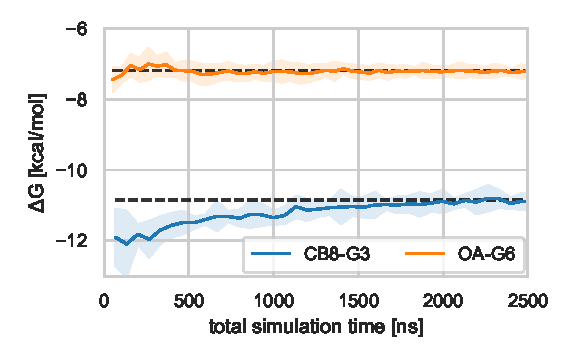
\includegraphics[width=0.90\linewidth]{figures/fig9_convergence/Figure.pdf}
    \caption{Average binding free energy of 5 replicate Hamiltonian replica exchange calculations as a function of total simulation time (i.e. the sum of the simulation time of all replicas) for the two host-guest systems CB8-G3 and OA-G3. Shaded areas represent 95\% confidence intervals around the mean computed from the 5 replicates data. The horizontal dashed lines show the final binding free energy prediction of the two calculations after a total of ~5230 ns for OA-G3 and ~6650 ns for CB8-G3. Longer correlation times in CB8-G3 cause the calculation to converge more slowly. The original data used to generate the plot can be found at \url{https://github.com/MobleyLab/SAMPL6/blob/master/host_guest/Analysis/SAMPLing/Data/reference_free_energies.csv}.
}
    \label{fig:freeenergytrajectories}
\end{figure}
%
\paragraph{Overlap matrix}
One way of assessing reliability of the calculations is checking the phase space overlap between neighboring $\lambda$-windows~\cite{wu2005phasespace,wu2005phasespacea}. For this purpose, a so-called overlap matrix can be used. This is a $K\times K$ matrix, where $K$ is the number of simulated states, i.e. $\lambda$s. Sufficient overlap is important for reweighting estimators such as BAR or MBAR, but cannot help assess reliability of estimates, when using TI. 
These matrices are graphical representations of the phase space overlap, i.e. the average probability that a sample generated at state $j$ can be observed at state $i$. As this probability is computed considering the samples from all states (and not just the adjacent states), the values in each row and column add up to 1. In this analysis, the goal is to ensure every state has overlap with its neighbors in both directions -- so that off-diagonal elements are significantly larger than zero. Usually this means the matrix should be at least tridiagonal.
%
Details on the calculation and properties of these matrices can be found elsewhere~\cite{klimovich2015guidelines}.
In an overlap matrix $\mathbf{O}$, the off-diagonal values (${O}_{i,j,i\ne j}$) are negatively correlated with the variance of the free energy difference. Accordingly, the uncertainty of the free energy difference between the states $i$ and $j$ will be smaller when ${O}_{i,j,i\ne j}$ is larger (and thus the values in the main diagonal (${O}_{i,j,i=j}$) are smaller). In order to obtain a reliable estimate of the free energy all neighbouring states must be connected, i.e. there must be sufficient overlap between the samples of these states (general description: ${O}_{i,j,i\ne j}\ge$ threshold).
However, due to the mathematical derivation it is difficult to explicitly describe the relation of the overlap matrix and the variance by formulae. Consequently, the threshold has to be derived empirically. It has been proposed that the values of the first off-diagonals (i.e. the diagonals above and below the main diagonal) should at least be 0.03 to obtain a reliable free energy estimate~\cite{klimovich2015guidelines}. Smaller values should be considered as a warning sign (see Fig.~\ref{fig:overlap}(C)), as the variance tends to be underestimated in case of poor overlap.

\begin{figure}
\includegraphics[width=0.95\columnwidth]{figures/fig12_overlap/Figure.pdf}
\caption{\label{fig:overlap} \textbf{Overlap matrices:} Visualising overlap matrices can help with assessing the quality of simulation data. (A) shows good overlap with all first off-diagonal entries well above 0.03, the suggested threshold, (B) is an example of mediocre overlap with good overlap at lower $\lambda$ values and poor overlap at high $\lambda$ values. (C)shows poor overlap resulting in disconnected simulations that should not be used for an MBAR estimation of free energies.}
\end{figure}

Fig.~\ref{fig:overlap} shows examples of good, mediocre and poor overlap (A), (B), and (C) respectively. For Fig.~\ref{fig:overlap}(A), the probability to find a sample from state $i$ in its neighbouring state $j$ is about 0.2 for all states adjacent to the main diagonal, and hence the overall connectivity is good. In the case of Fig.~\ref{fig:overlap}(B), the overlap is strongly diminishing in the lower right corner, raising concerns regarding the reliability of the free energy estimate obtained. For Fig.~\ref{fig:overlap}(C), the state at $\lambda$ index = 6 is connected to neither of its neighbouring states. While this does not necessarily imply that the result for this perturbation is wrong, the energy estimate must at least be considered as highly unreliable.
In order to overcome the issue of poor overlap in this example, additional sampling should be performed by introducing additional states, i.e. $\lambda$ windows.
%
Interestingly, as the variance is inversely correlated with the number of states\cite{klimovich2015guidelines}, it can in principle be reduced below any arbitrary threshold with enough simulation time and a large enough number of $\lambda$ windows. However, decreasing the variance to a value close to 0 is not feasible, as this approach would strongly increase the calculation time. While variance can be decreased both by increasing simulation length and by increasing the number of $\lambda$ values, if overlap is poor, the latter approach often has a larger immediate impact.  Specifically, often the goal is to adjust the $\lambda$ spacing to perform additional sampling in the areas of poor overlap, rather than using arbitrarily spaced windows. Different approaches are described in section~\ref{}) and more details can be found in the literature~\cite{dakka2018concurrent, hahn2019alchemical}.
%
In a nutshell, it must be ensured that the values of an overlap matrix in the first diagonals above and below the main diagonal are at least 0.03 in order to yield reliable results. 
%
There are several other parameters which should be investigated. Basic analysis of the trajectories should be performed to ensure that the ligand does not tumble out of the binding site by measuring its RMSD. Furthermore, distributions of the ligand's dihedral angles can be obtained and compared to experimental values. Thus, poorly sampled conformations can be identified and the issue can be adequately addressed, e.g. by prolonging the simulation time or choosing a different starting conformation. In general, running the same perturbation using different ligand poses may offer insights into whether the calculated free energies are dependent on the initial conformation.
Another easy check can be performed by comparing the results obtained by different free energy estimators (e.g. TI and MBAR). In principal, the outcomes of both estimators should be the same (within a certain range). Hence, if the outcomes deviate by more than a predefined threshold (e.g. 1.0 kcal/mol), the free energies are likely unreliable and further calculations are necessary.
%
\paragraph{Cycle closure error}
Relative free energy calculations, which compute the change in free energy on making a change to a molecule (e.g. adding a functional group to a ligand) may provide an additional opportunity for error/consistency checking. Particularly, such calculations are often done to span a graph or tree of free energy calculations~\cite{xu2019diffnet,wang2013modeling,liu2013lead} and in some cases the free energy change to go between molecules A and B can be obtained via multiple transformation pathways. This allows a type of consistency checking where we assess how much the free energy change for that transformation in practice differs from equivalence. Significant deviations from this typically indicate insufficient configurational sampling along the lambda schedule of one or more of the transformations involved.
%
This approach may be generalised to sets of connected transformations given the requirement that the sum of free energy changes along edges of a closed cycle should be zero. This analysis is called ``cycle closure''. In practice, such thermodynamic cycles do not actually sum to zero,  and deviations become increasingly large as the size of the cycle increases owing to propagation of error. Though no firm guidelines have emerged, it may be judicious to perform additional configurational sampling along edges of a network that are involved in cycles closing poorly. This may be done by extending simulations duration, or by averaging free energy changes over multiple repeats. The latter approach may yield more reproducible free energy changes, but at the expense of a stronger bias on the estimated free energies due to repeated use of the same input coordinates.
%
A scheme to reduce cycle closure errors is used in FEP+ whereby calculated free energy changes along the nodes of the network are re-sampled assuming estimates of the calculated free energy change along a node may be obtained from a Gaussian distribution centered on the estimated free energy change and with a standard deviation equal to the estimated standard deviation of the free energy change. The procedure then uses a Maximum likelihood method to find new sets of free energy changes that minimize cycle closure errors~\cite{wang2013modeling}. An alternative approach computes the free energy change between a target and reference compound as a weighted average over all unique paths in the network, with the weights derived from the propagated uncertainties of each node~\cite{mey2016blinded}. Approaches as illustrated by Yang et al. for perturbation map design can also be used to compute relative free energies between target and reference compounds~\cite{yang2020optimal}.
%
\paragraph{Reversible binding simulations}
An even more stringent test of the correctness of binding free energy calculations is to compare the results to the equilibrium binding constants derived from long timescale reversible binding simulations~\cite{pan2017quantitative}.  For small ligands with millimolar affinities, repeated binding to and unbinding from the protein can occur for a large number of times in a sufficiently long unbiased MD simulation (10-100$\mu$s), and the equilibrium binding constants can be straightforwardly computed from the ratio of bound to unbound fractions of the simulation time. The agreement between the binding free energy calculations and the reversible binding simulations--given the same system preparation and the same force field parameters--will strongly support the correctness of both calculations, as the same results are arrived at by two independent methods, and any discrepancy will suggest some systematic error in one, or both, of the two methods. As part of validation testing of alchemical free energy codes a benchmark set to compare alchemical and direct computation of equilibrium binding constant should become standard in future.
%
\subsection{Recommendations}
\todo[inline]{ASJSM:Maybe here we have a quick summary on what things should be checked for to make sure simulations are ok?}
\begin{itemize}
\item Examining output data for common problems with discussions of what exactly to plot or look at; examples of typical curves for dV/dlambda and free energy versus lambda, for example
\begin{itemize}
\item Make sure ligand doesn’t tumble out of binding site (Mey has observed this)
\item Significant discrepancies between different free energy estimators (TI, BAR, MBAR)
\item Poor replica mixing (for replica-exchange)
\item Correlation time as a function of lambda as it would be expected to be a smooth
\item Dependence on initial conformation
\item Torsional analysis: Is it stuck in specific states? Only very rarely transitions?
\item More “usual suspects”
\end{itemize}
\item Other considerations for many transformations
\end{itemize}
%
\subsection{Best practices for data representation}
\label{sec:plot_data}
Data generation and most adequate analysis isn't everything. As a practitioner of alchemical free energy simulations you are also encouraged to adhered to best practice for representing and plotting your results. We would encourage the following standard set of analyses and ways to represent data. 
\todo[inline]{JS: @everyone I suspect people will have strong opinions on this subject, feel free to include your own suggestions}
\paragraph{Statistics to include}
As with any modelling technique, misuse of statistical analysis can skew the perception of how well models perform in free energy predictions. First and foremost, error estimates should always be included on your predictions in whatever form you present your data (scatterplots, barplots, etc; see next paragraph). It is recommended to perform triplicates of your predictions at minimum to ensure some measure of reliability in your data, in part because analytical uncertainty estimates often underestimate the true statistical uncertainty, where this is not possible lower error bounds such as given by the MBAR estimator should be included. 
%
Because of the strong drug discovery context and the relevance of alchemical free energy predictions to structure activity relationship (SAR) projects, both the overall correlation of your predictions relative to experiment and the ability of your models to detect the best-scoring compounds (i.e. rankings) should be computed. Conventionally, this means including an R\textsuperscript{2} (or Pearson R -- 1 high correlation 0 no correlation -1 high anti-correlation) and a Kendall \texttau{} (with perfect ranking agreement when \texttau=1 and perfect disagreement when \texttau=-1) metric in your results. Additionally, practitioners may choose to include a Spearman \textrho{} as well. Brown et al.~\cite{brown2009healthy} have provided a useful analysis in terms of upper bounds of expected possible correlations between experiment and computation with a given potency range for the compounds. For example for potency ranges of 2 log units it would be impossible to get a higher correlation in R than 0.8 because of experimental uncertainties~\cite{brown2009healthy}. What often is neglected to include is an error analysis on correlation statistics that arise from the errors of both experimental and computed data. One way to include such error analysis for correlation metrics is using bootstrapping on the datasets. The D3R community challenges follows best practices on their data evaluation with readily available python scripts online~\cite{2018drugdata}, based on work by Pat Walters~\cite{walters2013what}. Other analysis software also provide similar functionality for bootstrapping datasets~\cite{antonia2019michellab}. 
%
Mean unsigned error (MUE, also called mean absolute error/MAE) is the another key statistic to include in your results. Even though some models' near-perfect correlation and ranking statistics might suggest excellent accuracy, MUE values can still be off multiple kcal/mol, providing important additional insight into performance. Furthermore, MUE allows for unbiased comparisons between predictive models as it is less sensitive to dataset size. Even though this section may serve as an introduction to the main statistical practices, the authors recommend further reading on evaluation of computational models \cite{jain2008recommendations, walters2013what, brown2009healthy, walterthoughts}.
%
\paragraph{Presenting your data}
Seeing as essentially all alchemical free energy prediction schemes are regression problems, the preferred type of plot is a scatter plot (see Figure \ref{fig:scatterplot_analysis}). Most alchemical FE projects will concern 10-50 ligands; any study with \textless10 ligands is more suitable for bar plots (with inclusion of error bars). Any study with \textgreater50 ligands should be trellised to not overestimate statistics. In that respect, it is bad practice to place multiple datasets on the same plot because this can suggest high model accuracy even though the individual models perform less well \cite{walterthoughts}.
%
Because we are interested mainly in the linear relationship between the alchemical FE predictions and the experimentally-determined affinity values, plots should be depicted with the same range on both axes (i.e. $x=y$). Furthermore, bounds should be depicted for the 1- and 2-kcal/mol confidence regions. These regions can serve as tools to communicate your model performance: any predictions inside the 1 kcal/mol region can be seen as highly reliable, any predictions inside the 2 kcal/mol region should be seen as somewhat reliable, and any predictions outside the confidence regions should be expected to be unreliable (and handled as outliers). In a drug discovery context, this type of data depiction may suggest the reliability of alchemical FE predictions in the project, and can give an idea of how trustworthy predictions can be for synthesis ideas. 
\begin{figure}
    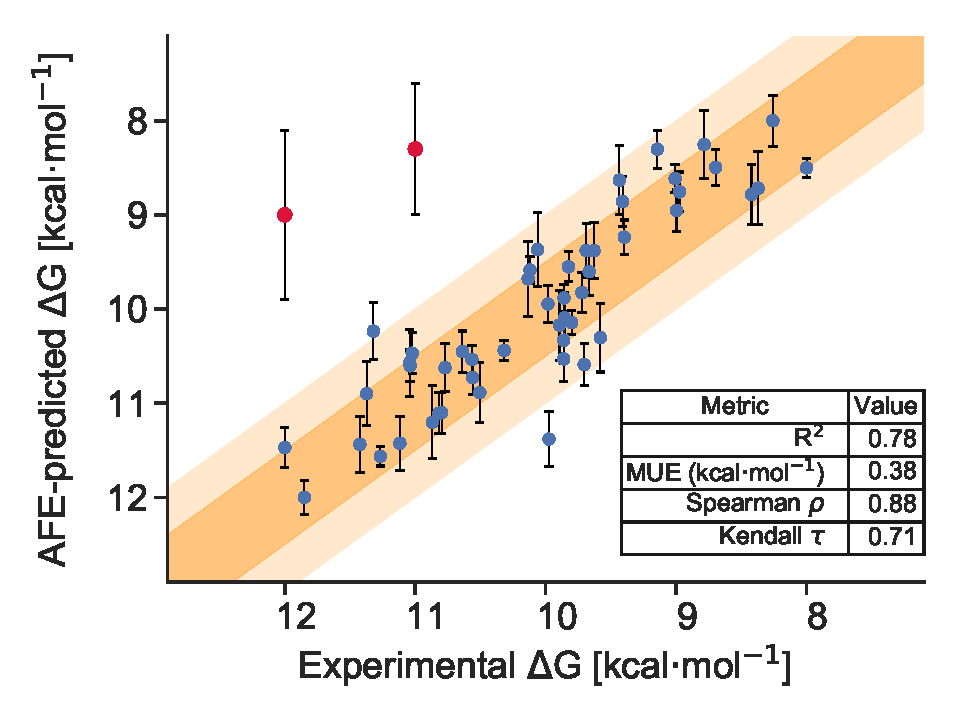
\includegraphics[width=0.95\linewidth]{figures/fig13_analysis_practices/Figure.pdf}
    \caption{Example of a well-depicted alchemical free energy prediction showing the relation between predicted and experimentally-determined Gibbs free energy in kcal/mol with standard errors as error bars. The two outliers (underestimations) are shown in red; the dark and light-orange regions depict the 1- and 2-kcal per mol confidence bounds.}
    \label{fig:scatterplot_analysis}
\end{figure}
An example of a best practice scatter comparison between computed and experimental values is shown in~\ref{fig:scatterplot_analysis}, highlighting outliers, error bars and confidence intervals. The data for this plot is artificially generated for illustration purposes.
%%%%%%%%%%%%%%%%%%%%%%%%%%%%%%%
% Conclusions                 %
%%%%%%%%%%%%%%%%%%%%%%%%%%%%%%%
\section{Conclusions}
\label{sec:conclusion}
Alchemical free energy calculations have seen a vast increase in popularity also in the pharmaceutical industry for structure based drug discovery~\cite{schindler2020largescale, sherborne2016collaborating, wagner2017computational}. Commercial products such as FEP+ and Flare, which provide a convenient user interface make the setup and use of these methods a lot easier~\cite{wang2015accurate}. Prospective prediction challenges such as the drug design data resource grand challenges provide a community driven platform to evaluate different free energy protocols against each other on unknown targets~\cite{gaieb2018d3r, gaieb2019d3r}. What has come out of these in the past is that SChrödinger's FEP+, performs similar when run by different participant groups~\cite{gaieb2018d3r}, but may not give the desired accuracy with RMSE errors larger than 1 kcal/mol. Other alchemical protocols performed similarly well. We hope that the best practice guide provides a set of tools that allow a better understanding of how to setup, run and interpret alchemical free energy calculations. The choice of the underlying simulation software is left to the user, but hopefully with this guide it is easier to assess whether the generated data is trustworthy or not. 
%
%%%%%%%%%%%%%%%%%%%%%%%%%%%%%%%
% Software                    %
%%%%%%%%%%%%%%%%%%%%%%%%%%%%%%%
\section{Available software -- a summary}
\todo[inline]{ASJSM: Expand and add more references. }
\label{sec:software}
There are several softwares availble for carrying out alchemical free energy calculations. In this section we discuss some of the popular commercial and free tools along with their features. 
\begin{itemize}
\item Commercial:
   \begin{itemize}
    \item FEP+ is a tool offered by Schr\"{o}dinger Inc. under a commercial license. It has an intuitive GUI which makes it easier for non-experts to run alchemical free energy calculations and analyze the results. It runs DESMOND MD package under the hood and hence parallelizes very well on the GPUs. 
    \item Flare is a commercial structure-based drug design software offered by Cresset. Similar to FEP+ it has an easily accessible user interface and strives to facilitate free energy calculations for non-experts while offering advanced users full control via a Python API. It only runs on GPUs, using CUDA or OpenCL.
    \item The molecular operating environment (MOE) offered by the Chemical Computing Group (CCG) has a tool for performing free energy calculations. It is build on AMBER-TI (cf. below).
    \end{itemize}
\item Free or low-cost for academics / commercial for industry:
	\begin{itemize}
	\item CHARMM has a variety of tools developed over the years. PERT module can be used to define initial and final states and define the intermediate lambda points. FREN and BAR modules can be used to analyze the data after the MD run. Lambda-dynamics based free energy calulation can be carried out using the BLOCK module.  
	\item TIES and AMBER FEW? (Peter Coveney)
	\item AMBER, including its new pmemd.cuda version support free energy calculation. 
	\end{itemize}
\item Free (libre) open source:
	\begin{itemize}
	\item PLUMED is an open source tool which enables the usage of a variety of MD engines. It is designed as a plugin for MD packages such that it analyzes the trajectory on the fly. It also offers a VMD based plugin for the computation of collective variables.   	
	\item SIRE  is a free, open source, multiscale molecular simulation framework, written to allow computational modellers to quickly prototype and develop new algorithms for molecular simulation and molecular design. 
	\item YANK is a tool developed by John Chodera and group on the top of OpenMM MD package. It allows the users to write their inputs in easy-to-use YAML format.
	\item GROMACS is a molecular simulation package with a significant number of free energy methods implementations. The LiveCOMS GROMACS tutorial has an example free energy calculation~\cite{lemkul2018From}.
	\item pmx for mutations
	\end{itemize}
\item Setup tools
	\begin{itemize}
	\item FESetup: AMBER, gromacs, Sire
	\item Lomap/Lomap2 : Relative alchemical transformation graph planning
	\item CHARMM-GUI is a web based tool for setting up a variety of MD simulations. It can be used to generate CHARMM scripts for solvation and ligand-binding free energy calculations.
	\end{itemize}
\item Analysis tools:
	\begin{itemize}
	\item Free Energy Workflows: Sire-specific free energy map analysis using weighted path averages
	\url{https://github.com/michellab/freenrgworkflows}
	\item Alchemlyb: Multipackage free energy analysis
	\url{https://github.com/alchemistry/alchemlyb}
	\item pymbar: MBAR implementation, but have to roll your own analysis wrapper
	\url{https://github.com/choderalab/pymbar}
	\end{itemize}
\end{itemize}

\section{Online resources}
\begin{itemize}
\item \url{http://www.ks.uiuc.edu/Training/Workshop/Urbana_2010A/lectures/TCBG-2010.pdf}
\item Basic Ingredients of Free Energy Calculations: A Review (\url{DOI: 10.1002/jcc.21450})
\item Good Practices in Free-Energy Calculations (\url{DOI: 10.1021/jp102971x})
\item Alchemical Free Energy Methods for Drug Discovery: Progress and Challenges (\url{doi: 10.1016/j.sbi.2011.01.011})
\item Alchemistry wiki: \url{http://www.alchemistry.org/wiki/Best_Practices}
\end{itemize}

\clearpage
\section{Benchmark Datasets}

\label{sec:benchmark}
\vspace{5mm}

\begin{table}
\caption{Overview of benchmark datasets}
\begin{tabular}{cccc}

\textbf{Publication} & \textbf{Targets} & \textbf{Ligands} & \textbf{Force Field} \\
\hline
\multicolumn{4}{|c|}{D3R Grand Challenges~\cite{D3R}} \\
\hline
GC3~\cite{gaieb2019d3r} & 6 & 266 & various \\
GC2~\cite{gaieb2018d3r} & 1 & 102 & various \\
GC2015~\cite{gathiaka2016d3r} & 2 & 215 & various \\
\hline
\multicolumn{4}{|c|}{SAMPL Challenges~\cite{SAMPL}} \\
\hline
SAMPL6~\cite{rizzi2018overview} & 3 & 21 & various \\
SAMPL5~\cite{yin2017overview} & 3 & 22 & various \\
SAMPL4~\cite{muddana2014sampl4} & 2 & 23 & various \\
\hline
\multicolumn{4}{|c|}{Schrödinger Datasets} \\
\hline
FEP+ Dataset~\cite{wang2015accurate} & 8 & 199 & OPLS2.1 \\
FEP+ Dataset~\cite{harder2016opls3} & 8 & 199 & OPLS3 \\
FEP+ Dataset~\cite{roos2019opls3e} & 8 & 199 & OPLS3e \\
FEP+ Dataset~\cite{song2019using} & 8 & 199 & AMBER18 \\
Fragment Optimization~\cite{steinbrecher2015accurate} & 8 & 96 & OPLS2.1 \\
Scaffold Hopping~\cite{wang2017accurate} & 6 & 21 & OPLS3 \\
Macrocycles~\cite{yu2017accurate} & 7 & 33 & OPLS3 \\
\hline
\multicolumn{4}{|c|}{Further Suggested Datasets} \\
\hline
Cucurbit[7]uril (CB7)~\cite{mobley2017predicting} & 1 & 15 & NA \\
Deep cavity cavitand~\cite{mobley2017predicting} & 2 & 19 & NA \\
T4 Lysozyme~\cite{mobley2017predicting} & 2 & 20 & NA \\
Merck benchmarking set~\cite{MCompChem2019Sep} & 5 & 169 & OPSL3 \\

\hline
\label{tab:benchmarks}
\end{tabular}
\end{table}

Several other case studies of alchemical calculations can be found in the review by Williams-Noonan et al.~\cite{williams-noonan2018free}. For comparison of FEP+ and Gromacs (using the AMBER99SB-ILDN and GAFF2 force field), cf. the recently published study by Pérez-Benito et al.~\cite{perez-benito2019predicting}.
An overview of further suggested benchmark sets can be found in the review by Mobley and Gilson~\cite{mobley2017predicting} or on \url{alchemistry.org}~\cite{alchemistry}. These include cyclodextrins, the Cytochrome C peroxidase (CCP) protein model binding site, thrombin and bromodomains as well as solvation benchmark sets~\cite{paliwal2011benchmark}. Further work on shared protein-ligand benchmark sets is ongoing at \url{https://github.com/openforcefield/PLBenchmarks}.

\section{Checklist}
\label{sec:checklist}
\todo[inline, color={green!20}]{JS: @everyone Please input your own suggestions, I made some points off the top of my head. Feel free to add helpful citations to any of the bullet points}
\todo[inline, color={green!20}]{JS: @self,ASJSM do some final formatting when text is complete.}

% This provides a checklist which
% - spans a full page
% - consists of multiple sub-checklists
% - exists on a separate page
% This style of checklist will be especially helpful if you want to encourage readers to print and use your checklist in practice, as they
% can easily print it without also printing other material from your manuscript. However, other styles of checklist are also possible (below).
% \begin{Checklists*}[p!]

% \begin{checklist}{Step 0 -- Know what you want to simulate }
% \textbf{What are the first questions that need addressing before setting up a molecular dynamics simulation}\\
% Extensive explanation for the checklist questions can be found in Section~\ref{sec:step0}.
% \begin{itemize}
% \item Can I get the required accuracy with the simulation I want to carry out?
% \item Have I properly prepared my protein and ligand systems?
% \item Does my system contain any groups that require custom parameters?
% \item What simulation protocol will provide the most evidence to answer my hypothesis?

% \item And finally
% \end{itemize}
% \end{checklist}

% \begin{checklist}{Simulation preparation}
% \textbf{How do I get started setting up an alchemical free energy calculation}
% Extensive explanation for the checklist questions can be found in Section~\ref{sec:prerequisites}.
% \begin{itemize}
% \item Have I followed the Best practices for biomolecular simulation set up?
% \item In a relative simulation, will I run into problems with clashing geometries in the ligand transformation or crystal waters?
% \end{itemize}
% \end{checklist}
% \end{Checklists*}

% \begin{Checklists*}[p!]
% \begin{checklist}{Absolute simulations}
% \textbf{What are the main things I need to consider for an absolute alchemical free energy calculation?}
% Extensive explanation for the checklist questions can be found in Section~\ref{sec:simulation_protocol_choice}.
% \begin{itemize}
% \item Topology
% \item Restraints
% \item Standard state handling
% \end{itemize}
% \end{checklist}

% \begin{checklist}{Relative simulations}
% \textbf{What are the main things I need to consider for an relative alchemical free energy calculation?}
% Extensive explanation for the checklist questions can be found in Section~\ref{sec:simulation_protocol_choice}.
% \begin{itemize}
% \item First thing
% \item Also remember
% \item And finally
% \end{itemize}
% \end{checklist}

% \begin{checklist}{Analysis}
% \textbf{This is all about analysis of the simulation}
% Extensive explanation for the checklist questions can be found in Section~\ref{sec:step4}.
% \begin{itemize}
% \item Are my simulations converged enough?
% \item Am I using the right analysis techniques?
% \end{itemize}
% \end{checklist}

% \end{Checklists*}

%Checklist:
\clearpage
%%%%%%%%%%%%%%%% 
%% Checklist-specific precommands:

\clearpage

\section*{Author Contributions}
%%%%%%%%%%%%%%%%
% This section mustt describe the actual contributions of
% author. Since this is an electronic-only journal, there is
% no length limit when you describe the authors' contributions,
% so we recommend describing what they actually did rather than
% simply categorizing them in a small number of
% predefined roles as might be done in other journals.
%
% See the policies ``Policies on Authorship'' section of https://livecoms.github.io
% for more information on deciding on authorship and author order.
%%%%%%%%%%%%%%%%
\todo[inline, color={green!20}]{ASJSM: @everyone, can you check your contribution is acknowledge and if not add the appropriate information. }
(Explain the contributions of the different authors here)
ASJSM: Coordinated the document, contributed to most sections, and co-designed figures ~\ref{} and created figures \ref{fig:fig_what_is_lambda},~\ref{fig:fig1_what_is_alchemy},~\ref{fig:overlap} and replotted~\ref{fig:automatic-equilibration-detection} and improved ~\ref{fig:fig_types_of_networks}.
JS: created figures \ref{fig:fig_what_is_alchemy},~\ref{fig:fig_binding_thermodynamic_cycle},~\ref{fig:fig_topology},~\ref{fig:fig_mcss},~\ref{fig:fig_types_of_networks},~\ref{fig:fig_absolute_thermodynamic_cycle},~\ref{fig:scatterplot_analysis}, the data representation section, the checklist and contributed to general formatting discussions and editing.
MK: Contributed to the Data Analysis section, provided the data for figure~\ref{fig:overlap} and helped edit the paper.
DLM: Contributed to the outline, drafted some of the sections, gave ideas on figures, and helped edit the paper.
GT: Contributed to introduction and drug discovery sections, and helped edit the paper.
AR: Created figure~\ref{fig:freeenergytrajectories}, contributed to section \ref{sec:simulation_protocol_choice}, and helped edit the paper.
MRS: Helped create figure~\ref{fig:fig_what_is_lambda}, wrote sections describing choices for alchemical pathways and analysis for free energy calculations.
LNN: Helped write the simulation length, stopping conditions, and information saving section.
BA: Helped write the uncertainty estimation, stopping conditions, and output analysis sections and created figure ~\ref{fig:convergence_forward_reverse}.
JM: Contributed to sections~\ref{subsec:reproducible},~\ref{sec:prerequisites},~\ref{} 4.2, 5.3, 6, 8.3.1, 8.3.2\
JDC: Wrote section~\ref{sec:decorrelating-samples} and~\ref{sec:automatic-equilibration-detection} discussed structure and design of the whole document, suggested Figs.~\ref{fig:fig_what_is_alchemy} and~\ref{fig:fig_sampling_scheme} \todo[inline, color={red!20}]{@JDC check info}
HX: Contributed section~\ref{subsec:accuracy}, to section~\ref{sec:relative-fe-protocol}, and to section~\ref{sec:are-they-good}.

% We suggest you preserve this comment:
For a more detailed description of author contributions,
see the GitHub issue tracking and changelog at \githubrepository.

\section*{Other Contributions}
%%%%%%%%%%%%%%%
% You should include all people who have filed issues that were
% accepted into the paper, or that upon discussion altered what was in the paper.
% Multiple significant contributions might mean that the contributor
% should be moved to authorship at the discretion of the a
%
% See the policies ``Policies on Authorship'' section of https://livecoms.github.io for
% more information on deciding on authorship and author order.
%%%%%%%%%%%%%%%

(Explain the contributions of any non-author contributors here)
% We suggest you preserve this comment:
For a more detailed description of contributions from the community and others, see the GitHub issue tracking and changelog at \githubrepository.



\section*{Potentially Conflicting Interests}
%%%%%%%
%Declare any potentially competing interests, financial or otherwise
%%%%%%%

Declare any potentially conflicting interests here, whether or not they pose an actual conflict in your view.
MK is employed by Cresset who recently released an commercial tool for performing alchemical free energy calculations.

\section*{Funding Information}
%%%%%%%
% Authors should acknowledge funding sources here. Reference specific grants.
%%%%%%%
ASJSM and JM acknowledge funding through an EPSRC flagship software grant: EP/P022138/1
MK acknowledges funding through Innovate UK by KTP partnership 011120.
AR acknowledges partial support from the Tri-Institutional Program in Computational Biology and Medicine and the Sloan Kettering Institute.

\bibliography{alchemical1,manual}

%%%%%%%%%%%%%%%%%%%%%%%%%%%%%%%%%%%%%%%%%%%%%%%%%%%%%%%%%%%%
%%% APPENDICES
%%%%%%%%%%%%%%%%%%%%%%%%%%%%%%%%%%%%%%%%%%%%%%%%%%%%%%%%%%%%

%\appendix


\end{document}
